\chapter{Expérimentations}     % numéroté
\label{chap:experiments}                   % étiquette pour renvois (à compléter!)

Nous avons testé notre approche de détection d'anomalies sur différents jeux de données. Nous avons également comparé nos résultats avec d'autres méthodes. Dans tous les cas, l'objectif est d'utiliser un jeu de données d'entraînement $\mathcal{X}$ contenant une proportion $p$ d'anomalies et de tester le modèle sur un jeu de données de test $\mathcal{X^*}$ contenant une proportion $p^*$ anomalies. Toutes les approches comparées sont des méthodes non-supervisées.

\section{Jeux de données} \label{exp:datasets}

Dans la première expérimentation, notre jeu de données a été créé à partir d'images réelles provenant de différentes sources de données, dont principalement \textit{ImageNet} \citep{deng2009imagenet}. Pour simplifier la terminologie, nous allons utiliser le terme \textit{ImageNet} pour caractériser le jeu de données de cette expérience. Dans la deuxième expérimentation, notre jeu de données a été créé à partir d'images tirées de \textit{MNIST} \citep{lecun2010mnist}. Dans les deux cas, les anomalies sont définies à partir des classes du jeu de données. Nous utiliserons les classes seulement dans le but de valider notre approche, et non dans l'entraînement du modèle.

Dans le cas du premier jeu de données, nous avons défini la classe dite "normale" à partir des images de \textit{Stanford Cars} \citep{KrauseStarkDengFei-Fei_3DRR2013}, soit des images de voitures. Les anomalies sont des images tirées aléatoirement des jeux de données \textit{Stanford Dogs} \citep{KhoslaYaoJayadevaprakashFeiFei_FGVC2011} et \textit{Indoor scene recognition} \citep{5206537}, des images de chiens et de pièces de bâtiment, respectivement. Ces images sont toutes tirées à la base de \textit{ImageNet}. La figure \ref{fig:imagenet} présente quelques exemples d'images provenant des 2 classes. Les images sont de type \textit{RGB} et ont toutes été re-dimensionnées en des images de 128 pixels par 128 pixels. Le tableau \ref{tab:dataset1} montre le nombre d'instances utilisées dans les jeux de données d'entraînement $\mathcal{X}$ et de test $\mathcal{X^*}$. On peut également y voir la proportion d'anomalies dans chaque ensemble selon 3 scénario différents. Le scénario de contamination appelé "Moins", signifie qu'il y a moins d'anomalies dans l'ensemble d'entraînement que dans l'ensemble de test. Le scénario appelé "égal" veut dire qu'il y a la même proportion d'anomalies dans les deux ensembles. Finalement, le scénario appelé "Plus", signifie qu'il y a plus d'anomalies dans l'ensemble d'entraînement que dans l'ensemble de test.

\begin{figure}[htb]
	\centering
	\begin{subfigure}{6cm}
		\centering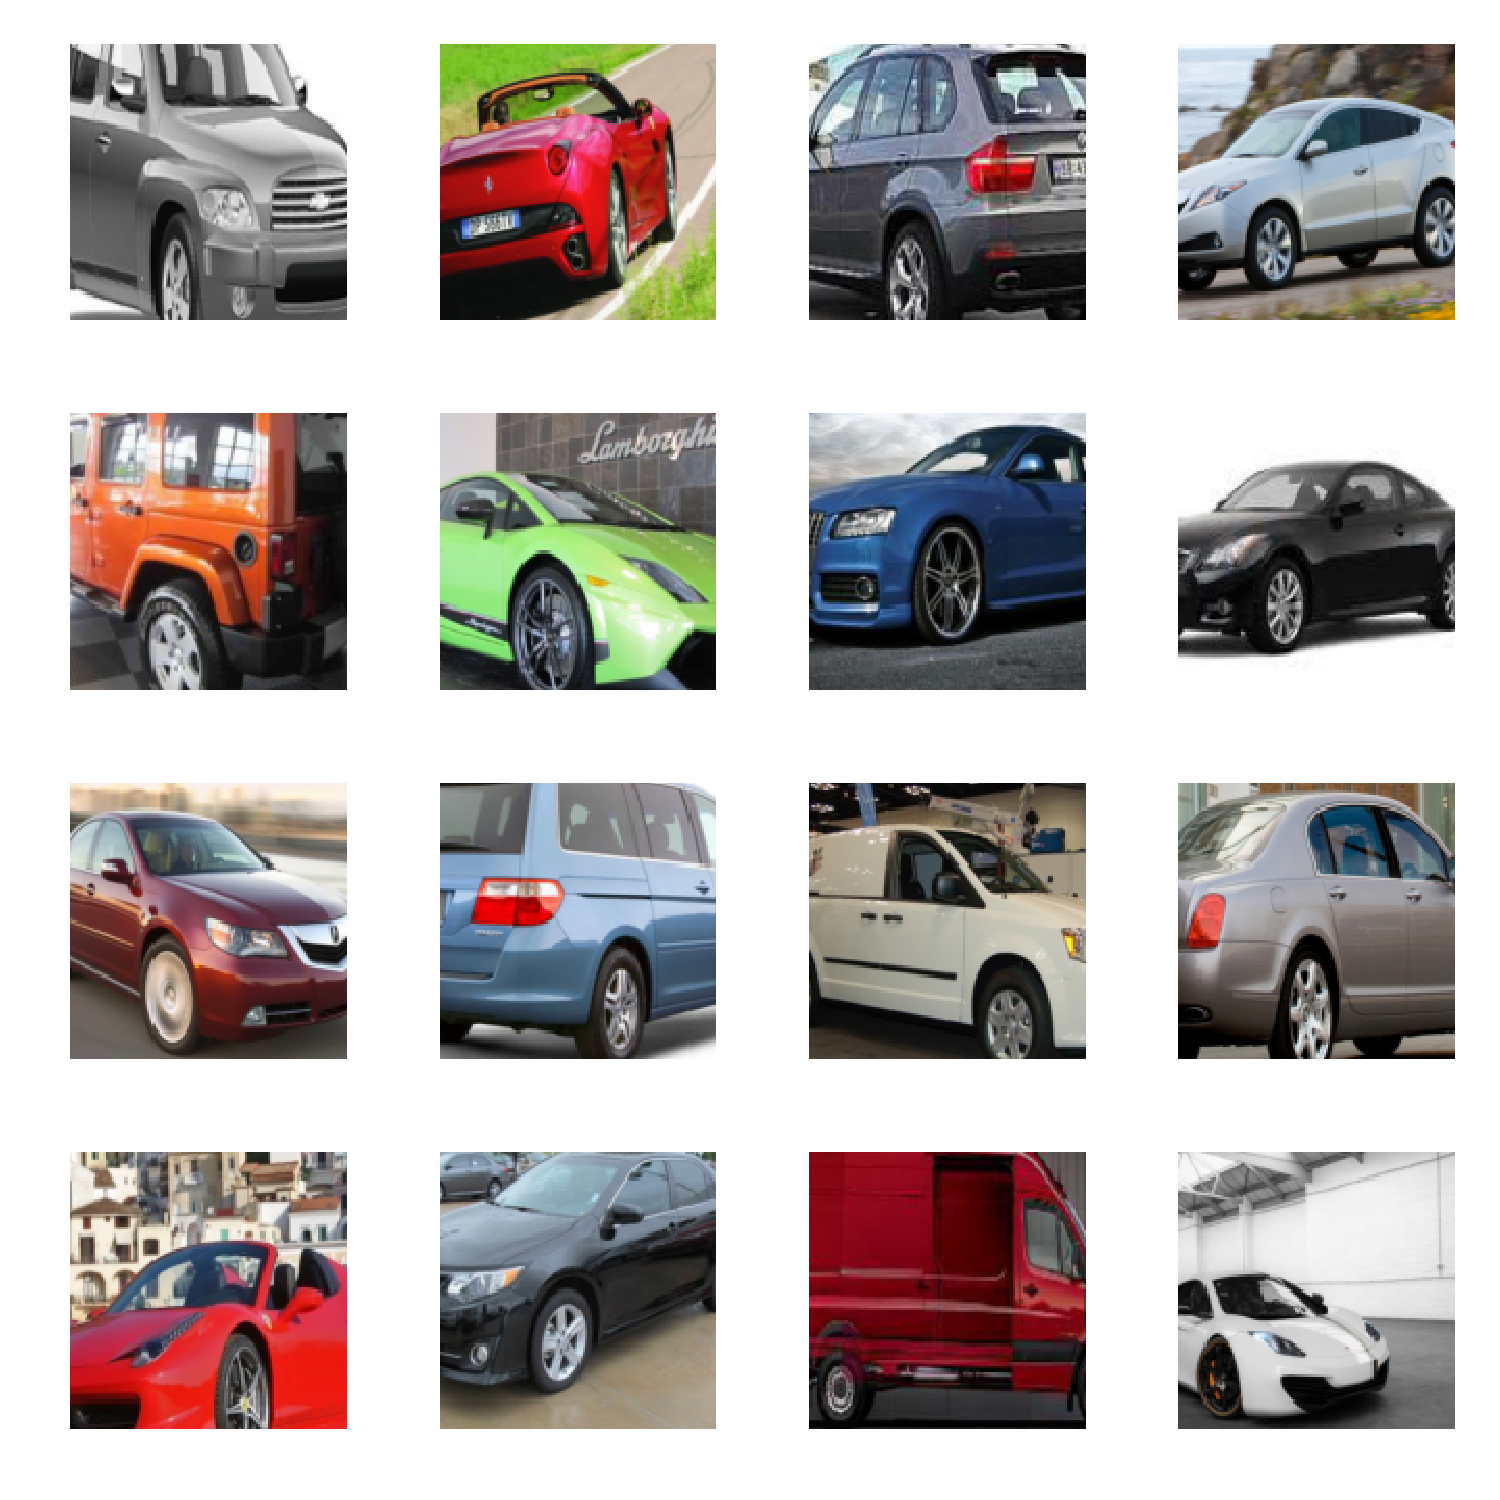
\includegraphics[width=6cm]{images/imagenet-inliers}
		\caption{Classe "normale"}
	\end{subfigure}
	\begin{subfigure}{6cm}
		\centering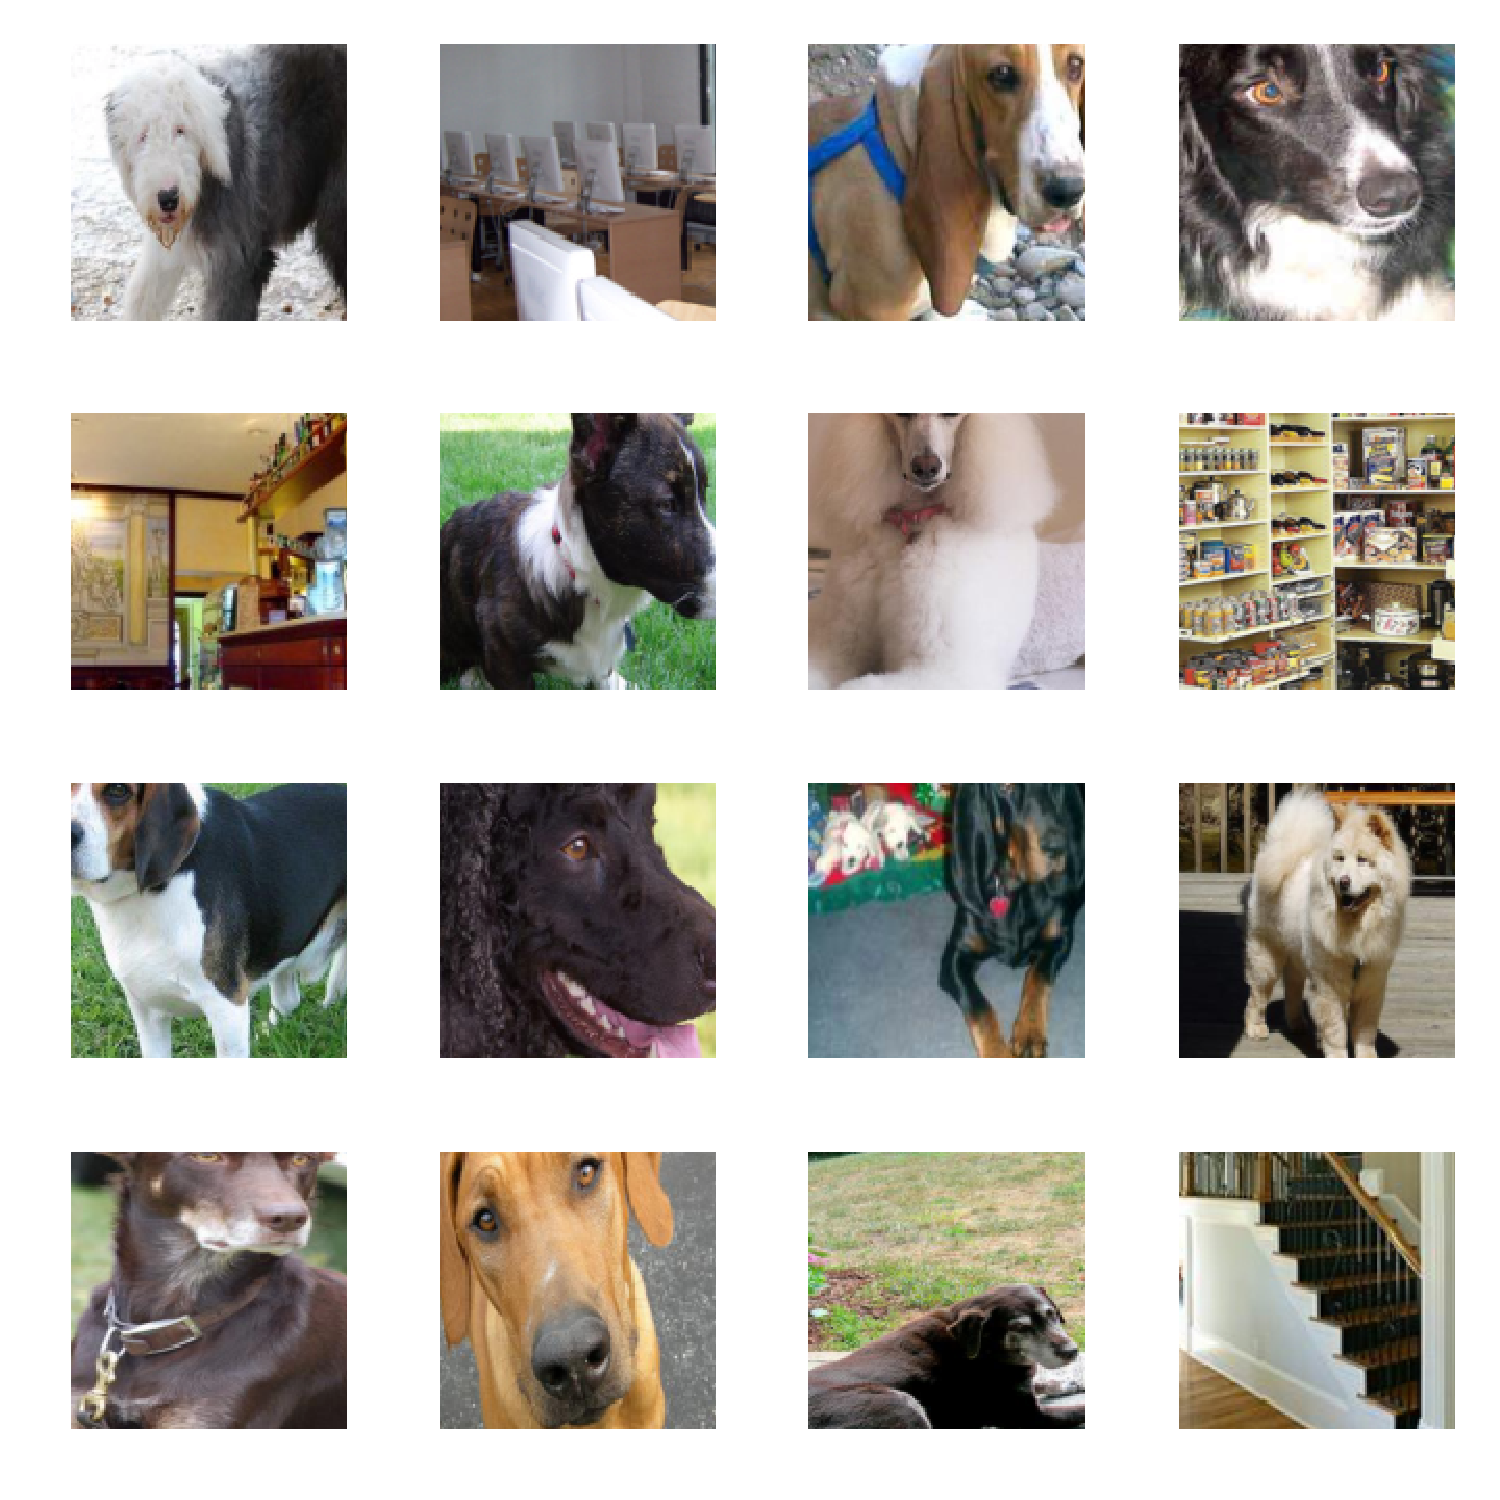
\includegraphics[width=6cm]{images/imagenet-outliers}
		\caption{Classe d'anomalies}
	\end{subfigure}
	\caption{Exemples d'images pour notre jeu de données d'images réelles tirées de \textit{ImageNet}. La figure à gauche (a) correspond à des exemples de la classe dite "normale" et le volet de droite (b) correspond à des exemples de la classe d'anomalies.}
	\label{fig:imagenet}
\end{figure}

\begin{table}[h]
	\centering
	\caption{Description des 2 ensembles de données pour le jeu de données de \textit{ImageNet}.}
	\begin{tabular}{| c | c | c | c |}
		\hline
		\rowcolor{Gray}
		Contamination & Ensemble de données  & Nombre d'instances & Pourcentage d'anomalies  \\
		\hline
		\multirow{2}{*}{Moins} 
		& $\mathcal{X}$ & 10000 & 10\%  \\
		& $\mathcal{X^*}$  & 1000 & 1\%  \\ 
		\midrule
		\multirow{2}{*}{Égal} 
		& $\mathcal{X}$ & 10000 & 5\%  \\
		& $\mathcal{X^*}$  & 1000 & 5\%  \\ 
		\midrule
		\multirow{2}{*}{Plus} 
		& $\mathcal{X}$ & 10000 & 1\%  \\
		& $\mathcal{X^*}$  & 1000 & 10\%  \\ 
		\midrule
	\end{tabular}
	\label{tab:dataset1}
\end{table}

Dans le cas du deuxième jeu de données, la classe "normale" est définie en prenant une catégorie du jeu de données \textit{MNIST}, soit un chiffre de 0 à 9. Nous avons ensuite défini 3 scénarios de test différents. Ces 3 scénarios se différencient par le nombre de classes que nous catégorisons comme des anomalies. Pour chacun de ces 3 scénarios, nous avons testé 2 catégories "normales" différentes, ce qui donne au total 6 scénarios de test. Ces scénarios sont définis plus en détails dans le tableau \ref{tab:mnist_scenarios}. La figure \ref{fig:mnist} présente quelques exemples d'images, considérant que le chiffre 0 est la classe "normale" et tous les autres chiffres sont des anomalies. Les images sont de type noir et blanc et sont toutes de dimensions 28 pixels par 28 pixels. Le tableau \ref{tab:dataset2} montre le nombre d'instances utilisées dans les jeux de données d'entraînement $\mathcal{X}$ et de test $\mathcal{X^*}$. Il montre également les proportions d'anomalies dans chaque ensemble, de la même manière qu'avec le jeu de données \textit{ImageNet}. Pour chacun des niveaux de contamination, les 6 différents scénarios du tableau \ref{tab:mnist_scenarios} ont été testés.

\begin{table}[h]
	\centering
	\caption{Description des 2 ensembles de données pour le jeu de données provenant de \textit{MNIST}.}
	\begin{tabular}{| a | a | a |}
		\hline
		\rowcolor{Gray}
		Scénario de test  & Chiffre "normal" & Chiffres "anormaux"  \\
		\hline
		1 & 1 & 5  \\
		2 & 1 & 5,9  \\
		3  & 1 & 0,2,3,4,5,6,7,8,9 \\ 
		4 & 6 & 8  \\
		5 & 6 & 3,8  \\
		6  & 6 & 0,1,2,3,4,5,7,8,9  \\ \hline
	\end{tabular}
	\label{tab:mnist_scenarios}
\end{table}

\begin{figure}[htb]
	\centering
	\begin{subfigure}{6cm}
		\centering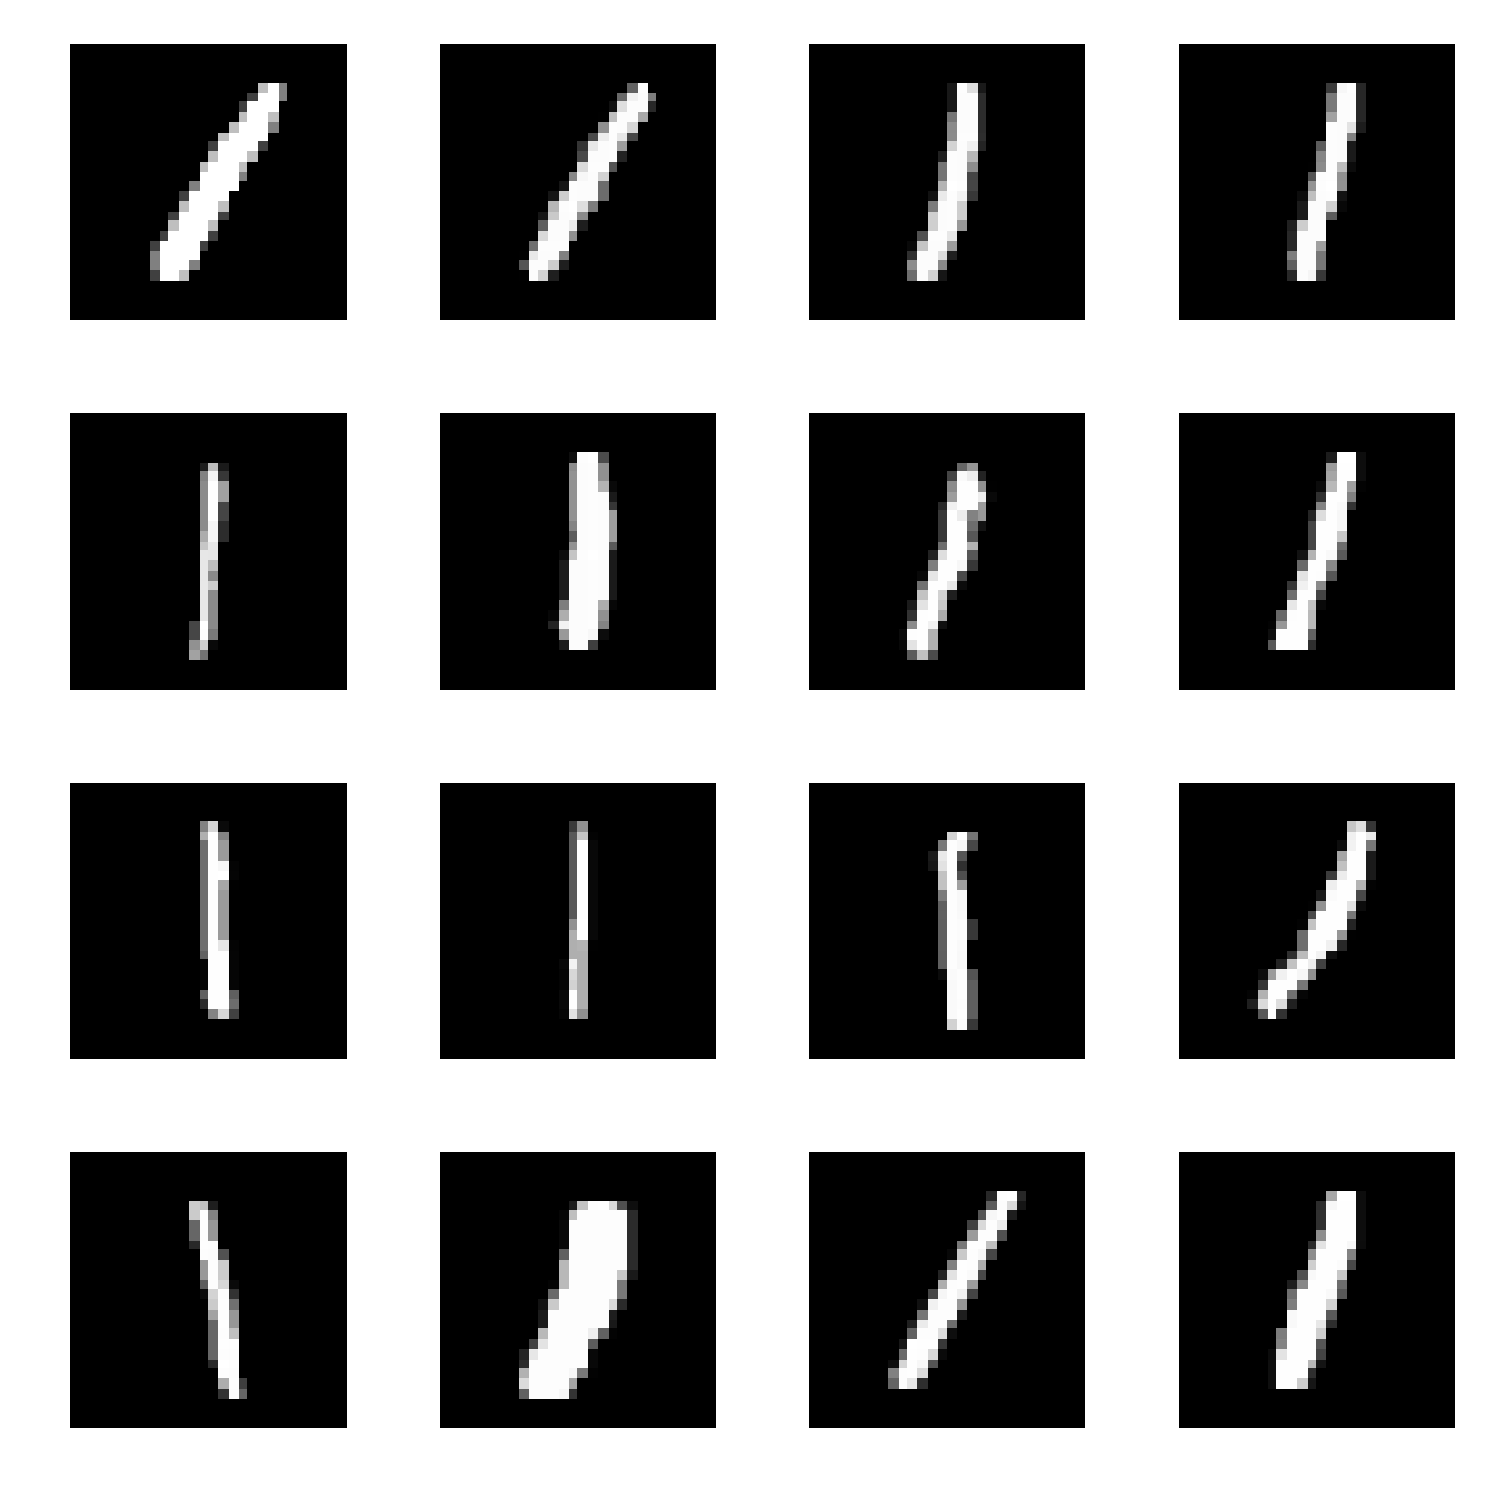
\includegraphics[width=6cm]{images/mnist-inliers}
		\caption{Classe normale}
	\end{subfigure}
	\begin{subfigure}{6cm}
		\centering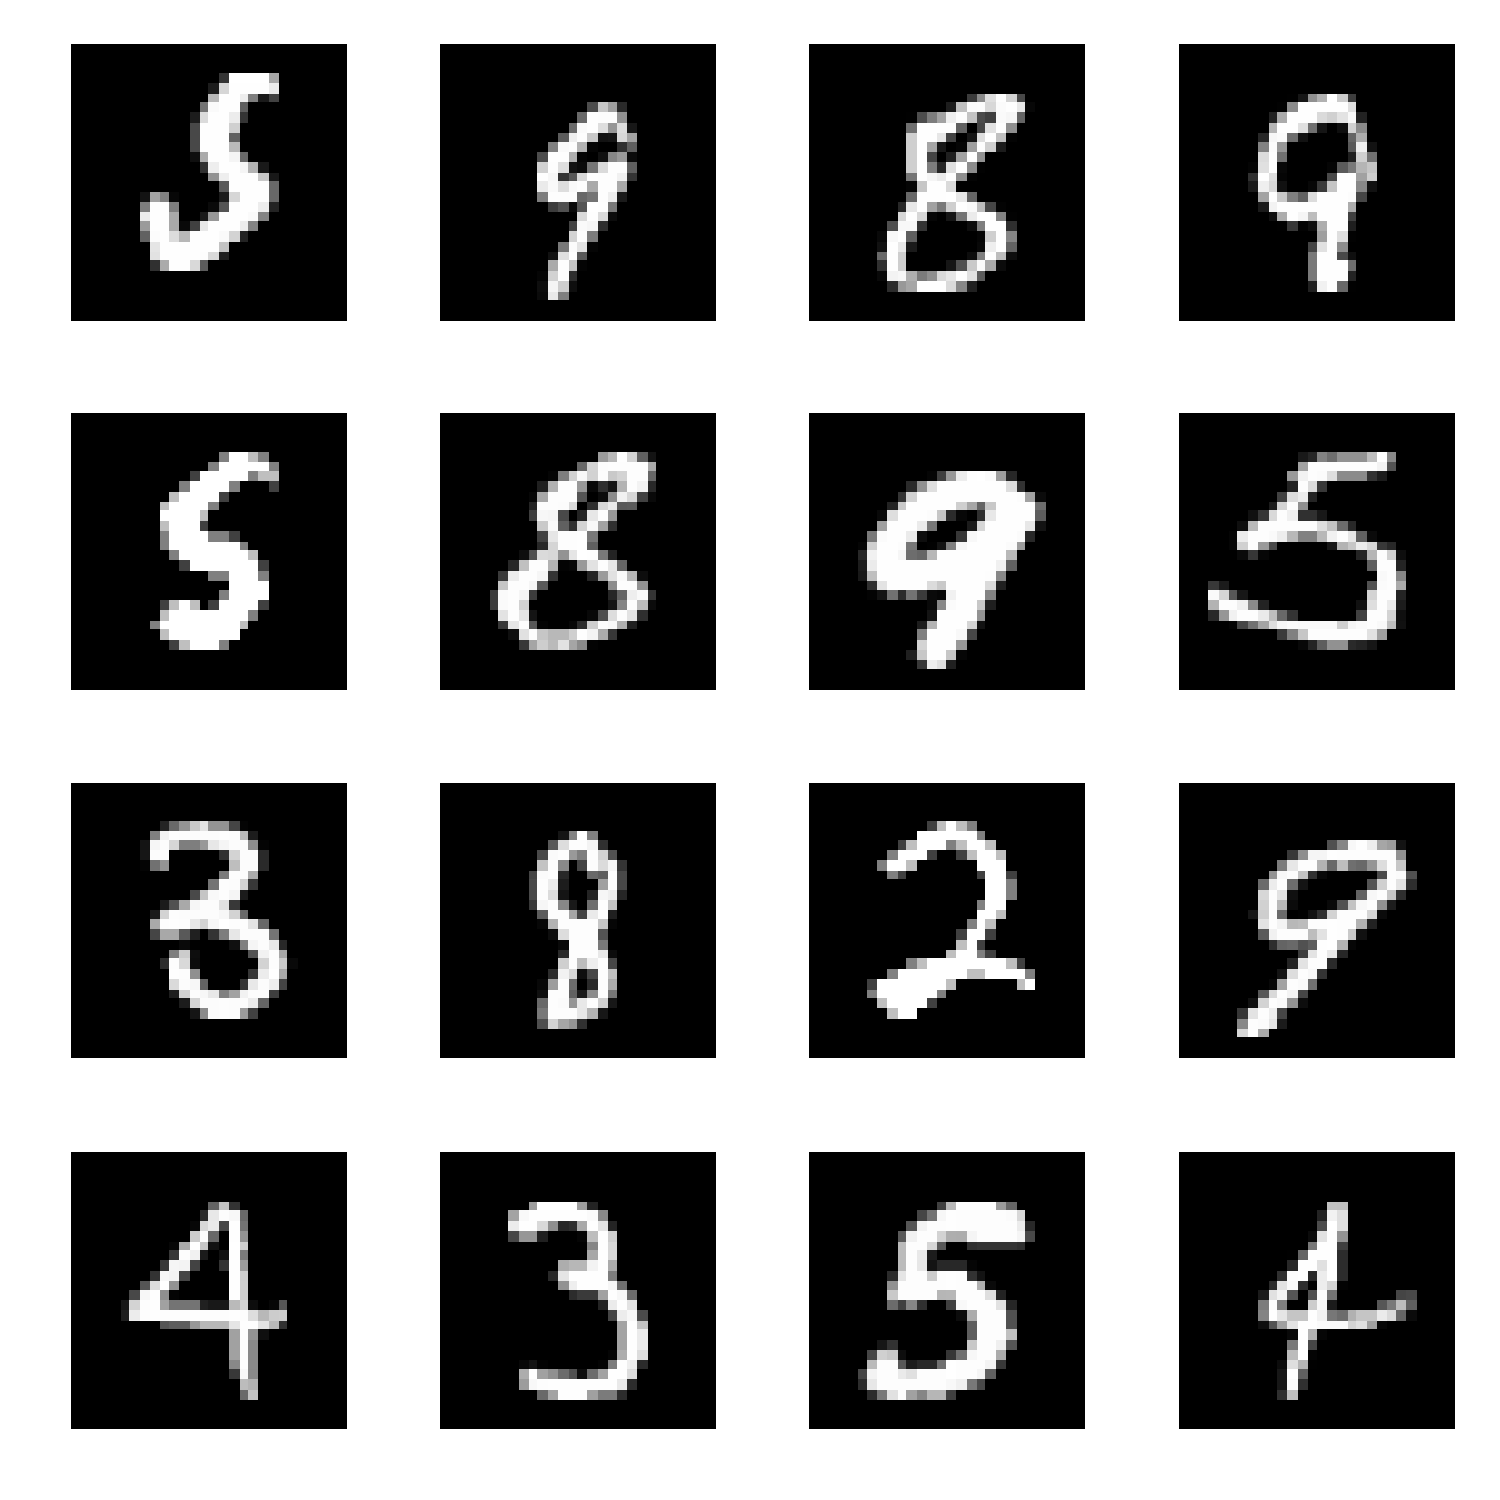
\includegraphics[width=6cm]{images/mnist-outliers}
		\caption{Classe d'anomalies}
	\end{subfigure}
	\caption{Exemples d'images pour notre jeu de données \textit{MNIST}. La figure à gauche (a) correspond à des exemples de la classe "normale" et le volet de droite (b) correspond à des exemples de la classe d'anomalies. Il s'agit plus particulièrement du scénario de test 3.}
	\label{fig:mnist}
\end{figure}

\begin{table}[h]
	\centering
	\begin{tabular}{| c | c | c | c |}
		\hline
		\rowcolor{Gray}
		Contamination & Ensemble de données  & Nombre d'instances & Pourcentage d'anomalies  \\
		\hline
		\multirow{2}{*}{Moins} 
		& $\mathcal{X}$ & 4000 & 10\%  \\
		& $\mathcal{X^*}$  & 800 & 1\%  \\ 
		\midrule
		\multirow{2}{*}{Égal} 
		& $\mathcal{X}$ & 4000 & 5\%  \\
		& $\mathcal{X^*}$  & 800 & 5\%  \\ 
		\midrule
		\multirow{2}{*}{Plus} 
		& $\mathcal{X}$ & 4000 & 1\%  \\
		& $\mathcal{X^*}$  & 800 & 10\%  \\ 
		\midrule
	\end{tabular}
	\caption{Description des 2 ensembles de données pour le jeu de données de \textit{MNIST}.}
	\label{tab:dataset2}
\end{table}

\section{Méthodes testées}

Dans un premier temps, nous avons testé notre approche de détection d'anomalies basée sur des autoencodeurs variationnels, que nous appellerons DA-VAE (section \ref{DA_VAE}). Dans un deuxième temps, nous avons testé trois autres approches. Tout d'abord, nous avons testé une méthode basée sur une analyse en composantes principales (ACP), décrite plus en détails dans la section \ref{acp}. Ensuite, nous avons testé une approche basée sur un autoencodeur traditionnel avec des couches de convolutions (AE), décrite dans la section \ref{AE}. Finalement, nous avons testé une dernière approche utilisant le même autoencodeur variationnel que dans l'approche DA-VAE, mais en appliquant l'algorithme de détection d'anomalies \textit{Isolation Forest} \citep{4781136} sur les représentations latentes (ISOF-VAE). Cette méthode est décrite plus en détails dans la section \ref{isof_vae}. Ces quatre différentes approches et leurs détails d'entraînement sont approfondis dans les prochaines sous-sections.

\subsection{Détails sur la méthode DA-VAE} \label{DA_VAE}

La section \ref{chap:methodologie} décrit en détails le fonctionnement de l'approche que nous proposons. Par contre, certains détails concernant l'entraînement de l'autoencodeur variationnel ont été omis jusqu'à maintenant. Tout d'abord, il faut mentionner que l'architecture du réseau de neurones est différente pour chacun des 2 jeux de données décrits à la section \ref{exp:datasets}.

Dans le cas du jeu de données provenant de \textit{ImageNet}, nous avons défini 4 couches de convolution pour l'encodeur et 4 couches de convolution transposée pour le décodeur. Chaque couche de convolution est suivie d'une normalisation par min-lot (\textit{batch normalization}) et d'une fonction d'activation de type \textit{ReLU}. Juste avant de définir les couches de vecteurs latents $\boldsymbol{\mu}$ et $\boldsymbol{\sigma}$, le résultat de la dernière couche de convolution de l'encodeur, de dimensions $(512 \times 16 \times 16)$, est aplati en un vecteur de longueur 131 072. Les couches de vecteurs latents $\boldsymbol{\mu}$ et $\boldsymbol{\sigma}$ sont ensuite obtenue via une couche linéaire. La couche latente possède 25 dimensions. Nous avons entraîné le réseau sur 25 itérations complètes des données tout en ayant 130 observations par mini-lot. L'algorithme d'optimisation est celui de \textit{Adam} \citep{kingma2014method} et le taux d'apprentissage est de 0.001. Finalement, le niveau de filtration $\alpha$ appliqué sur le jeu de données de test est le même que la proportion de contamination dans le jeu de donnée de test. La figure \ref{fig:archit_imagenet} présente en détails les différentes couches de l'encodeur et du décodeur.

\begin{figure}[htbp]
	\begin{subfigure}{12cm}
		\begin{tikzpicture}[shorten >=1pt,draw=black!50, node distance=\layersep, square/.style={regular polygon,regular polygon sides=4}]
		\tikzstyle{box}=[square,fill=white,minimum size=2cm,inner sep=-20pt, draw=black, text width=2.5cm, text centered]
		\tikzstyle{annot} = [text width=4em, text centered]
		
		% Draw different layers
		\node[box,fill=yellow!50] (input) at (0,0) {\tiny Entrée \\ $3 \PLH 128 \PLH 128$};
		\node[box,fill=green!50] (conv1) at (2,0) {\tiny Conv-2D $16 \PLH 128 \PLH 128$};
		\node[box,fill=green!50] (conv2) at (4,0) {\tiny Conv-2D $128 \PLH 64 \PLH 64$};
		\node[box,fill=green!50] (conv3) at (6,0) {\tiny Conv-2D $256 \PLH 32 \PLH 32$};
		\node[box,fill=green!50] (conv4) at (8,0) {\tiny Conv-2D $512 \PLH 16 \PLH 16$};
		\node[box,fill=yellow!50] (flatten) at (10,0) {\tiny Flatten \\ $1 \PLH 131 072$};
		\node[box,fill=black!30] (mu) at (12,1.2) {\tiny Linéaire \\ $1 \PLH 25$};
		\node[box,fill=black!30] (sigma) at (12,-1.2) {\tiny Linéaire \\ $1 \PLH 25$};
		\node[box,fill=yellow!50] (z) at (14,0) {\tiny $z$ \\ $1 \PLH 25$};
		
		% Draw arrows
		\path[->, line width=1mm] (input) edge (conv1);
		\path[->, line width=1mm] (conv1) edge (conv2);
		\path[->, line width=1mm] (conv2) edge (conv3);
		\path[->, line width=1mm] (conv3) edge (conv4);
		\path[->, line width=1mm] (conv4) edge (flatten);
		\path[->, line width=1mm] (flatten) edge (mu);
		\path[->, line width=1mm] (flatten) edge (sigma);
		\path[->, line width=1mm] (mu) edge (z);
		\path[->, line width=1mm] (sigma) edge (z);
		
		\node[annot,above of=mu, node distance=1cm] (h2) {$\mu$};
		\node[annot,above of=sigma, node distance=1cm] (h3) {$\sigma$};
		
		\end{tikzpicture}
		\caption{Architecture de l'encodeur}
	\end{subfigure}
	\begin{subfigure}{12cm}
		\vspace{0.75cm}
		\begin{tikzpicture}[shorten >=1pt,draw=black!50, node distance=\layersep, square/.style={regular polygon,regular polygon sides=4}]
		\tikzstyle{box}=[square,fill=white,minimum size=2cm,inner sep=-20pt, draw=black, text width=2.5cm, text centered]
		\tikzstyle{annot} = [text width=4em, text centered]
		
		% Draw different layers
		\node[box,fill=yellow!50] (z) at (0,0) {\tiny $z$ \\ $1 \PLH 25$};
		\node[box,fill=black!30] (linear3) at (2,0) {\tiny Linéaire \\ $1 \PLH 131 072$};
		\node[box,fill=yellow!50] (unflatten) at (4,0) {\tiny Unflatten \\ $512 \PLH 16 \PLH 16$};
		\node[box,fill=green!50] (deconv1) at (6,0) {\tiny Deconv-2D $256 \PLH 32 \PLH 32$};
		\node[box,fill=green!50] (deconv2) at (8,0) {\tiny Deconv-2D $128 \PLH 64 \PLH 64$};
		\node[box,fill=green!50] (deconv3) at (10,0) {\tiny Deconv-2D $16 \PLH 128 \PLH 128$};
		\node[box,fill=green!50] (deconv4) at (12,0) {\tiny Deconv-2D $3 \PLH 128 \PLH 128$};
		\node[box,fill=yellow!50] (output) at (14,0) {\tiny Sortie \\ $3 \PLH 128 \PLH 128$};
		
		% Draw arrows
		\path[->, line width=1mm] (z) edge (linear3);
		\path[->, line width=1mm] (linear3) edge (unflatten);
		\path[->, line width=1mm] (unflatten) edge (deconv1);
		\path[->, line width=1mm] (deconv1) edge (deconv2);
		\path[->, line width=1mm] (deconv2) edge (deconv3);
		\path[->, line width=1mm] (deconv3) edge (deconv4);
		\path[->, line width=1mm] (deconv4) edge (output);
		
		\end{tikzpicture}
		\vspace{0.15cm}
		\caption{Architecture du décodeur}
	\end{subfigure}
	\caption{Architecture du modèle DA-VAE pour le jeu de données \textit{ImageNet}. Les blocs représentent les couches du réseau. Les blocs jaunes représentent les couches où il n'y a pas de paramètres à optimiser. Les blocs verts sont des couches de convolution ou déconvolution et les blocs gris sont des couches linéaires. }
	\label{fig:archit_imagenet}
\end{figure}

Pour le jeu de données provenant de \textit{MNIST}, nous avons défini 3 couches de convolution pour l'encodeur et 3 couches de convolution transposée pour le décodeur. Nous avons fait le choix de mettre moins de couches que dans le cas du jeu de données \textit{ImageNet} en raison de la complexité moins importante des données.  Chaque couche de convolution est suivie d'une fonction d'activation de type \textit{ReLU}. Chaque couche de convolution de l'encodeur est également suivie d'un \textit{max pooling} de dimensions $2 \times 2$. Juste avant de définir les couches de vecteurs latents $\boldsymbol{\mu}$ et $\boldsymbol{\sigma}$, le résultat de la dernière couche de convolution de l'encodeur, de dimensions $(64 \times 4 \times 4)$, est aplati en un vecteur  de longueur 1024. Les couches de vecteurs latents $\boldsymbol{\mu}$ et $\boldsymbol{\sigma}$ sont ensuite obtenues via une couche linéaire. La couche latente possède 25 dimensions. Nous avons entraîné le réseau pendant 75 itérations complètes des données tout en ayant 256 observations par mini-lot. L'algorithme d'optimisation est celui de \textit{Adam} et le taux d'apprentissage est de 0.001. Finalement, le niveau de filtration $\alpha$ appliqué sur le jeu de données de test est le même que la proportion de contamination dans l'ensemble de données de test. La figure \ref{fig:archit_mnist} présente en détails les différentes couches de l'encodeur et du décodeur.

\begin{figure}[htbp]
	\begin{subfigure}{12cm}
		\begin{tikzpicture}[shorten >=1pt,draw=black!50, node distance=\layersep, square/.style={regular polygon,regular polygon sides=4}]
		\tikzstyle{box}=[square,fill=white,minimum size=2cm,inner sep=-19pt, draw=black, text width=2.5cm, text centered]
		\tikzstyle{annot} = [text width=4em, text centered]
		
		% Draw different layers
		\node[box,fill=yellow!50] (input) at (0,0) {\tiny Entrée \\ $1 \PLH 28 \PLH 28$};
	\node[box,fill=green!50] (conv1) at (2,0) {\tiny Conv-2D + \\ Max-pooling $16 \PLH 14 \PLH 14$};
		\node[box,fill=green!50] (conv2) at (4,0) {\tiny Conv-2D + \\ Max-pooling $32 \PLH 7 \PLH 7$};
		\node[box,fill=green!50] (conv3) at (6,0) {\tiny 0-padding \\ $32 \PLH 8 \PLH 8$};
		\node[box,fill=green!50] (conv4) at (8,0) {\tiny Conv-2D + \\ Max-pooling $64 \PLH 4 \PLH 4$};
		\node[box,fill=yellow!50] (flatten) at (10,0) {\tiny Flatten \\ $1 \PLH 1024$};
		\node[box,fill=black!30] (mu) at (12,1.2) {\tiny Linéaire \\ $1 \PLH 25$};
		\node[box,fill=black!30] (sigma) at (12,-1.2) {\tiny Linéaire \\ $1 \PLH 25$};
		\node[box,fill=yellow!50] (z) at (14,0) {\tiny $z$ \\ $1 \PLH 25$};
		
		% Draw arrows
		\path[->, line width=1mm] (input) edge (conv1);
		\path[->, line width=1mm] (conv1) edge (conv2);
		\path[->, line width=1mm] (conv2) edge (conv3);
		\path[->, line width=1mm] (conv3) edge (conv4);
		\path[->, line width=1mm] (conv4) edge (flatten);
		\path[->, line width=1mm] (flatten) edge (mu);
		\path[->, line width=1mm] (flatten) edge (sigma);
		\path[->, line width=1mm] (mu) edge (z);
		\path[->, line width=1mm] (sigma) edge (z);
		
		\node[annot,above of=mu, node distance=1cm] (h2) {$\mu$};
		\node[annot,above of=sigma, node distance=1cm] (h3) {$\sigma$};
		
		\end{tikzpicture}
		\caption{Architecture de l'encodeur}
	\end{subfigure}
	\begin{subfigure}{12cm}
		\vspace{0.75cm}
		\begin{tikzpicture}[shorten >=1pt,draw=black!50, node distance=\layersep, square/.style={regular polygon,regular polygon sides=4}]
		\tikzstyle{box}=[square,fill=white,minimum size=2cm,inner sep=-20pt, draw=black, text width=2.5cm, text centered]
		\tikzstyle{annot} = [text width=4em, text centered]
		
		% Draw different layers
		\node[box,fill=yellow!50] (z) at (0,0) {\tiny $z$ \\ $1 \PLH 25$};
		\node[box,fill=black!30] (linear3) at (2,0) {\tiny Linéaire \\ $1 \PLH 1024$};
		\node[box,fill=yellow!50] (unflatten) at (4,0) {\tiny Unflatten \\ $64 \PLH 4 \PLH 4$};
		\node[box,fill=green!50] (deconv1) at (6,0) {\tiny Deconv-2D \\ $64 \PLH 8 \PLH 8$};
		\node[box,fill=green!50] (deconv2) at (8,0) {\tiny Deconv-2D \\ $32 \PLH 16 \PLH 16$};
		\node[box,fill=green!50] (deconv3) at (10,0) {\tiny Deconv-2D \\ $16 \PLH 28 \PLH 28$};
		\node[box,fill=green!50] (deconv4) at (12,0) {\tiny Conv-2D \\ $1 \PLH 28 \PLH 28$};
		\node[box,fill=yellow!50] (output) at (14,0) {\tiny Sortie \\ $1 \PLH 28 \PLH 28$};
		
		% Draw arrows
		\path[->, line width=1mm] (z) edge (linear3);
		\path[->, line width=1mm] (linear3) edge (unflatten);
		\path[->, line width=1mm] (unflatten) edge (deconv1);
		\path[->, line width=1mm] (deconv1) edge (deconv2);
		\path[->, line width=1mm] (deconv2) edge (deconv3);
		\path[->, line width=1mm] (deconv3) edge (deconv4);
		\path[->, line width=1mm] (deconv4) edge (output);
		
		\end{tikzpicture}
		\vspace{0.15cm}
		\caption{Architecture du décodeur}
	\end{subfigure}
	\caption{Architecture du modèle DA-VAE pour le jeu de données provenant de \textit{MNIST}. Les blocs représentent les couches du réseau. Les blocs jaunes représentent les couches où il n'y a pas de paramètres à optimiser. Les blocs verts sont des couches de convolution ou déconvolution et les blocs gris sont des couches linéaires.}
	\label{fig:archit_mnist}
\end{figure}

\subsubsection{Horaire du paramètre $\beta$} \label{beta_schedule}

Dans les deux expériences différentes, nous avons traité le paramètre $\beta$ d'une manière particulière. En effet, étant donné que nous utilisons des $\beta$-VAE, nous devons définir un paramètre $\beta$ qui donne plus ou moins d'importance à la composante de perte associée au critère de Kulbach-Leibler (voir section \ref{beta-vae}). Dans notre cas, nous n'avons pas conservé ce paramètre $\beta$ fixe tout au long de l'entraînement. Pour l'entraînement des 2 différents jeux de données, nous avons donc mis en place un horaire du paramètre $\beta$ selon l'itération d'entraînement (ou \textit{epoch}). Cet horaire n'est pas le même selon le jeu de données et a été choisi en se basant sur la section 3.1 de l'article \cite{bowman-etal-2016-generating}. Ce qui est proposé dans cet article est de commencer l'entraînement en attribuant un poids de zéro à la perte de KL. Pendant les premières itérations, le réseau va donc optimiser ses paramètres en fonction de la composante de reconstruction seulement. Par la suite, on augmente le paramètre $\beta$ pour régulariser le modèle et ainsi rapprocher les paramètres $\boldsymbol{\mu}$ et $\boldsymbol{\sigma}$ de ceux de la $N(0,I)$. Le tableau \ref{tab:betas} présente les paramètres $\beta$ utilisés selon l'itération (\textit{epoch}) d'entraînement et le jeu de données.

\begin{table}[h]
	\centering
	\caption{Horaire des paramètres $\beta$ pour le jeu de données provenant de \textit{ImageNet} et le jeu de données provenant de \textit{MNIST}.}
	\begin{tabular}{| a | a | a |}
		\hline
		\rowcolor{Gray}
		Itération  & $\beta_{ImageNet}$ & $\beta_{MNIST}$  \\
		\hline
		$[0,5]$ & 0 & 0  \\
		$[6,10]$  & 100 & 10  \\
		$[11,\infty]$  & 10 & 1  \\ \hline

	\end{tabular}
	\label{tab:betas}
\end{table}

L'intuition derrière l'horaire établi est de contrôler le modèle dans les premières itérations pour éviter d'accorder trop d'importance, et ce trop rapidement, à la composante de régularisation KL. Cela pourrait avoir comme conséquence de nuire au reste de l'optimisation et à l'apprentissage de la composante de reconstruction.	

\subsection{Détails sur la méthode ACP} \label{acp}

Une première approche testée pour comparer nos résultats consiste à effectuer une analyse en composantes principales (ACP). L'objectif premier de cette technique non-supervisée est réduire la dimension d'un ensemble de données en conservant le plus d'information possible. Cela permet d'ailleurs de représenter les données dans un espace plus simple sous formes de représentations latentes. Il est aussi possible de reconstruire ces représentations dans les dimensions originales, et ainsi de calculer un score d'anomalie basé sur la capacité de bien reconstruire. Dans cette méthode, les valeurs et vecteurs propres de la matrice de covariance des variables standardisées 

\begin{equation} \label{eq1}
	\begin{split}
		\hat{\text{var}}(\mathbf{X}) & = \frac{1}{n}\mathbf{X}^{T}\mathbf{X},
	\end{split}
\end{equation}


nous permettent d'obtenir une projection de cette matrice dans un espace à plus petites dimensions. La matrice $\mathbf{X}$ correspond aux données standardisées qu'on cherche à réduire la dimension. La matrice de vecteurs propres $\mathbf{V}$ est de dimensions $p \times d$, où $p$ correspond au nombre de variables de la matrice $\mathbf{X}$ et $d$ correspond au nombre de composantes principales conservées dans l'espace réduit. La représentation en dimension réduite, soit $\mathbf{Z}$, est obtenue par le produit de $\mathbf{X}\mathbf{\mathbf{V}}$. Finalement, la reconstruction dans l'espace original, $\hat{\mathbf{X}}$, est donnée par

\begin{gather*}
	\hat{\mathbf{X}} = \mathbf{Z}\mathbf{V}^{T}=\mathbf{X}\mathbf{V}\mathbf{V}^{T}.
\end{gather*}

Étant donné que nos données sont des images, ou des matrices en plusieurs dimensions, nous avons aplati chacune des entrées pour obtenir des vecteurs. Dans le cas des images en couleur provenant de \textit{ImageNet}, nous avons d'abord aplati chacun des canaux RGB. Ensuite, nous avons fait une analyse en composantes principales sur chaque canal RGB séparément. Chaque canal image est de dimensions $1 \times 128 \times 128$, ce qui veut dire que nous obtenons un vecteur de longueur 16 384 pour chaque ACP. Pour les images provenant de \textit{MNIST}, les images sont de dimensions $1 \times 28 \times 28$, ce qui nous donne des vecteurs de longueur 784. Cette vectorisation est nécessaire dans le cas de l'analyse en composantes principales puisque chaque observation de $\mathbf{X}$ doit être représentée comme un vecteur.

Pour trouver les anomalies, nous avons utilisé l'erreur de reconstruction entre les données originales $(x^{*(j)})_{j=1}^k$ et
leur reconstruction $(\hat{x}^{*(j)})_{j=1}^k$ basée uniquement sur un certain nombre de composantes principales. Dans nos expériences, ce nombre de composantes principales à été établi afin d'obtenir une projection conservant approximativement 80\% de la variance originale des données. Nous avons utilisé l'erreur quadratique moyenne comme erreur de reconstruction. Une observation $x^{*(j)}$ est considérée comme une anomalie au niveau de filtration $\alpha$ si

\begin{gather} \label{eq:anomalie_mse}
l(x^{*(j)}, \hat{x}^{*(j)}) > t_{1-\alpha}(L(\mathcal{X}, \hat{\mathcal{X}})),
\end{gather}

où $l(x^{*(j)}, \hat{x}^{*(j)})$ correspond à l'erreur de reconstruction pour l'observation $i$ du jeu de données test $\mathcal{X^*}$ et $t_{1-\alpha}(L(\mathcal{X}, \hat{\mathcal{X}}))$ correspond au percentile $1-\alpha$ de l'ensemble des erreurs de reconstruction sur le jeu de données d'entraînement $\mathcal{X}$. Le niveau de filtration $\alpha$ choisi est le même que la proportion de contamination dans l'ensemble de données de test. Dans le cas de l'ACP appliquée sur \textit{ImageNet}, nous avons calculé l'erreur de reconstruction sur chaque canal indépendamment pour ensuite prendre la moyenne des 3 erreurs de reconstruction. 

 Pour le jeu de données \textit{ImageNet}, nous avons conservé le nombre de composantes principales nous permettant de conserver exactement 80 \% de la variabilité pour chaque canal RGB. Ce nombre de composantes principales peut donc varier légèrement selon le canal et l'échantillonnage du jeu de données. Ces nombres de composantes conservées peuvent varier entre 90 et 110. Pour le jeu de données \textit{MINST}, nous avons toujours conservé les 30 premières composantes principales. Cela nous permet de conserver approximativement  80 \% de la variabilité, selon l'échantillonnage. 

\subsection{Détails sur la méthode AE} \label{AE}

Une deuxième approche testée consiste à utiliser un autoencodeur traditionnel et de se servir de l'erreur de reconstruction comme score d'anomalie. Pour cette approche, nous avons utilisé les mêmes architectures que celles définies dans la section \ref{DA_VAE}, mais sans les couches linéaires latentes du réseau DA-VAE. Par exemple, pour l'autoencodeur appliqué sur les images provenant de \textit{ImageNet}, nous avons conservé les 4 premières couches de convolution et avons ensuite appliqué les 4 dernières couches de convolution transposée immédiatement après. Il n'y a donc pas de vectorisation qui est nécessaire. 

Nous avons utilisé l'erreur quadratique moyenne comme erreur de reconstruction. Les anomalies du jeu de données test $\mathcal{X^*}$ sont donc prédites de façon similaire à ce qui est présenté à l'équation \ref{eq:anomalie_mse}. Le niveau de filtration $\alpha$ choisi est le même que la proportion de contamination dans le jeu de données de test.

\subsection{Détails sur la méthode ISOF-VAE} \label{isof_vae}

Finalement, nous avons testé une dernière approche qui consiste à utiliser différemment les représentations latentes du réseau entraîné avec l'approche DA-VAE. Au lieu de calculer une distance de Kullback-Leibler entre chaque représentation latente et une distribution normale $N(0,I)$, nous utiliserons ici les représentations latentes pour entraîner l'algorithme \textit{Isolation Forest}. Cet algorithme non-supervisé, principalement utilisé en détection d'anomalie, utilise plusieurs arbres de décisions binaires regroupés dans ce qu'on appelle une fôret d'arbres. Chacun des arbres est entraîné sur un certains nombre d'observations tiré au hasard et avec remise. De plus, il est également possible de tirer au hasard un certains nombre de variables pour entraîner chacun des arbres. Ce processus est très similaire à ce qui est fait en apprentissage supervisé avec les forêts aléatoires.\citep{Statistics01randomforests}. L'hypothèse de base de cet algorithme quant aux anomalies est fondée autour du fait qu'elles sont peu nombreuses et possèdent des caractéristiques différentes des observations "normales". Sachant cette hypothèse, ces anomalies sont susceptibles d'être isolées dans les premières séparations des arbres de décisions. Pour déterminer si une observation est isolée, on calcule le nombre de nœuds à parcourir dans l'arbre pour atteindre cette observation. Plus ce chemin est petit, plus l'observation risque d'être une anomalie.

Afin d'obtenir un score d'anomalie comparable à notre niveau de filtration $\alpha$, nous avons légèrement transformé le score d'anomalie calculé par l'algorithme. Pour une observation donnée, le score d'anomalie $S$  calculé par l'algorithme est obtenu en prenant la moyenne du nombre de nœuds parcouru dans chacun des arbres de la forêt pour atteindre cette observation. Plus ce score est petit, plus l'observation est susceptible d'être isolée et d'être considérée "anormale". Pour être en mesure de comparer ce score avec notre niveau de filtration, nous avons d'abord calculé ce score pour chacune des $n$ observations de notre jeu de données d'entraînement, ce que nous appelons l'ensemble $S_{\mathcal{X}} = \{S^{(1)}, ..., S^{(n)}\}$. Nous définissons également $S^{'}_{\mathcal{X}}$ comme l'ensemble $S_{\mathcal{X}}$ ordonné en ordre croissant.  Ensuite, nous avons défini notre propre score d'anomalie $S^*(\cdot)$ pour une observation du jeu de donnée de test $x^{*(j)}$ comme suit,

\begin{gather}
	S^*(x^{*(j)}) = \frac{rang_{S^{'}_{\mathcal{X}}}(S^{(j)})}{n},
\end{gather}

où $rang_{S^{'}_{\mathcal{X}}}(S^{(j)})$ correspond au rang du score $S^{(j)}$ de l'observation $x^{*(j)}$ dans l'ensemble ordonné $S^{'}_{\mathcal{X}}$. Ce score $S^*(x^{*(j)})$, peut être comparé à notre niveau de filtration $\alpha$. Ce niveau de filtration choisi est le même que la proportion de contamination dans le jeu de données de test.

\section{Résultats}

Pour comparer les différentes méthodes, nous avons utilisé 3 métriques différentes. La première est l'aire sous la courbe ROC. Cette métrique nous permet de faire abstraction du seuil de filtration $\alpha$. Ensuite, nous avons également choisi les métriques de précision et de rappel, qui prennent en considération un certain seuil, $\alpha$ dans notre cas. Nous avons entraîné et testé les algorithmes à 20 reprises, ce qui nous permet de calculer une moyenne et une mesure de dispersion, soit l'écart-type, autour de chacune des métriques. Pour les 20 expérimentations, l'échantillonnage des jeux de données de test et d'entraînement est refait. La variabilité des résultats entre les 20 expérimentations est expliquée par 3 composantes :

\begin{enumerate}
	\item L'échantillonnage des jeux de données;
	\item L'initialisation des paramètres et l'optimisation par descente du gradient dans les réseaux de neurones;
	\item La composante stochastique dans la représentation latente du VAE.
\end{enumerate}

La première composante, soit l'échantillonnage des jeux de données, affecte les 4 différents algorithmes. La deuxième composante, soit l'initialisation des paramètres et l'optimisation par descente du gradient, n'affecte que les méthodes reliées à des réseaux de neurones: DA-VAE(\ref{DA_VAE}), AE (\ref{AE}) et ISOF-VAE (\ref{isof_vae}). La composante stochastique dans l'optimisation par descente du gradient est reliée au fait que le jeu de données d'entraînement est divisé en sous-ensembles, aussi appelés mini-lot, qui sont définis aléatoirement. Ces sous-ensembles sont utilisés pour calculer les pertes sur lesquelles on calcule les dérivés permettant de mettre à jour les paramètres de l'autoencodeur à chaque itération d'entraînement. L'optimisation globale du réseau de neurones peut donc emprunter des chemins légèrement différents avec une même initialisation. Finalement, la troisième composante concerne seulement les deux méthodes utilisant l'autoencodeur variationnel: DA-VAE et ISOF-VAE. Comme il a été expliqué à la section \ref{background-vae}, la représentation latente de l'autoencodeur variationnel est obtenue en combinant les paramètres des couches $\boldsymbol{\mu}$ et $\boldsymbol{\sigma}$ du modèle ainsi que la simulation d'une loi $N(0,I)$.

Nous ne faisons qu'une présentation brute des résultats dans cette sous-section et nous en faisons l'analyse et la discussion à la sous-section \ref{discussion}.
  

\subsection{Résultats sur \textit{ImageNet}}

Le tableau \ref{tab:results_cars} synthétise les résultats obtenus sur le jeu de données provenant de \textit{ImageNet}. On peut y voir les résultats pour les 4 approches différentes, pour les 3 scénarios de contamination ainsi que pour les 3 métriques choisies. Nous avons mis en gras les résultats de la méthode nous apparaissant la plus adaptée pour chaque métrique. Ce choix est basé en grande partie sur la valeur moyenne de la métrique.

\begin{table}[h]
	\centering
	\caption{Résultats selon les métriques d'aire sous la courbe ROC, de précision et de rappel pour les différentes expérimentations concernant le jeu de données \textit{ImageNet}.}
	\begin{tabular}{c|c|c c c c}
		\toprule
		Contamination & Métrique & ACP & AE & ISOF-VAE & DA-VAE \\
		\hline
		\multirow{3}{*}{Moins} 
		& ROC & 0.406 $\pm$ 0.086 & 0.549 $\pm$ 0.090 & 0.886 $\pm$ 0.059 & $\mathbf{0.935 \pm 0.042}$  \\ 
		& $\text{Précision}_{\alpha=0.01}$ & 0.016 $\pm$ 0.028 & 0.019 $\pm$ 0.041 & 0.325 $\pm$ 0.268 & $\mathbf{0.400 \pm 0.231}$  \\
		& $\text{Rappel}_{\alpha=0.01}$ & 0.025 $\pm$ 0.043 & 0.020 $\pm$ 0.040 & 0.089 $\pm$ 0.079 & $\mathbf{0.120 \pm 0.093}$  \\
		\midrule
		\multirow{3}{*}{Égal} 
		& ROC & 0.426 $\pm$ 0.040 & 0.584 $\pm$ 0.050 & 0.859 $\pm$ 0.037 & $\mathbf{0.923 \pm 0.018}$  \\ 
		& $\text{Précision}_{\alpha=0.05}$ & 0.040 $\pm$ 0.023 & 0.136 $\pm$ 0.041 & 0.499 $\pm$ 0.086 & $\mathbf{0.504 \pm 0.057}$  \\
		& $\text{Rappel}_{\alpha=0.05}$ & 0.052 $\pm$ 0.029 & 0.144 $\pm$ 0.048 & 0.461 $\pm$ 0.087 & $\mathbf{0.576 \pm 0.065}$  \\
		\midrule
		\multirow{3}{*}{Plus} 
		& ROC & 0.429 $\pm$ 0.030 & 0.568 $\pm$ 0.047 & 0.811 $\pm$ 0.045 & $\mathbf{0.920 \pm 0.019}$  \\ 
		& $\text{Précision}_{\alpha=0.1}$ & 0.111 $\pm$ 0.025 & 0.202 $\pm$ 0.035 & 0.437 $\pm$ 0.044 & $\mathbf{0.449 \pm 0.030}$  \\
		& $\text{Rappel}_{\alpha=0.1}$ & 0.137 $\pm$ 0.036 & 0.231 $\pm$ 0.042 & 0.594 $\pm$ 0.078 & $\mathbf{0.798 \pm 0.058}$  \\
		\midrule
	\end{tabular} 
	\label{tab:results_cars}
\end{table}

Dans la figure \ref{fig:auc_cars}, on peut voir plus en détails la distribution des résultats obtenus sur les 20 expérimentations via des graphiques en boîtes et moustaches.

\begin{figure}[H]
	\centering
	\begin{subfigure}{12cm}
		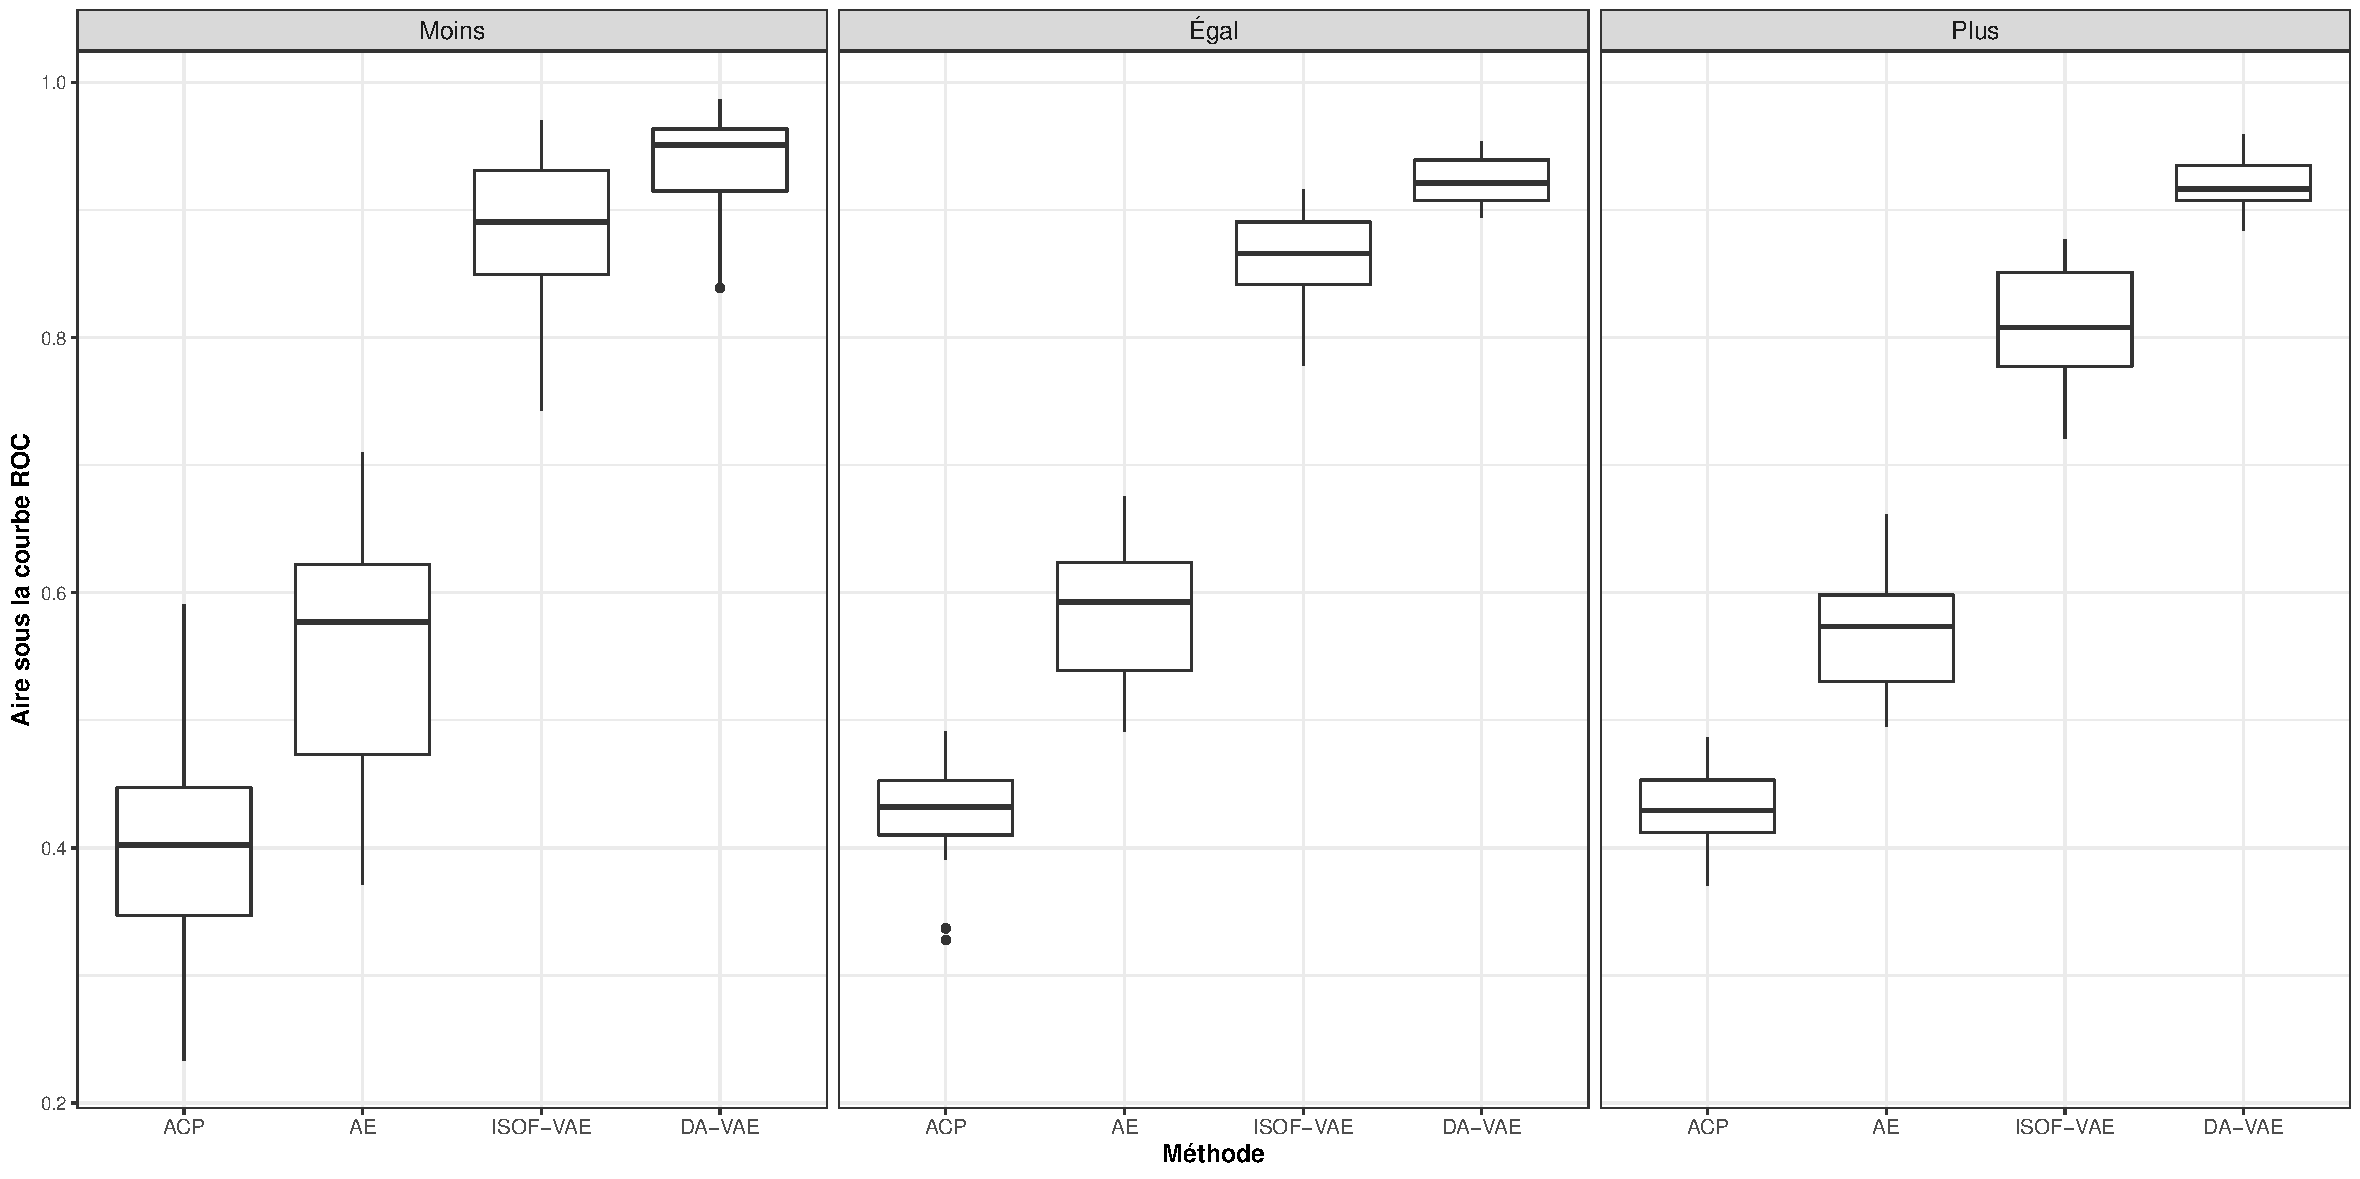
\includegraphics[width=12cm]{images/images_boxplots/auc_cars.pdf}
		\caption{Résultats en aire sous la courbe ROC}
	\end{subfigure}
	\begin{subfigure}{12cm}
		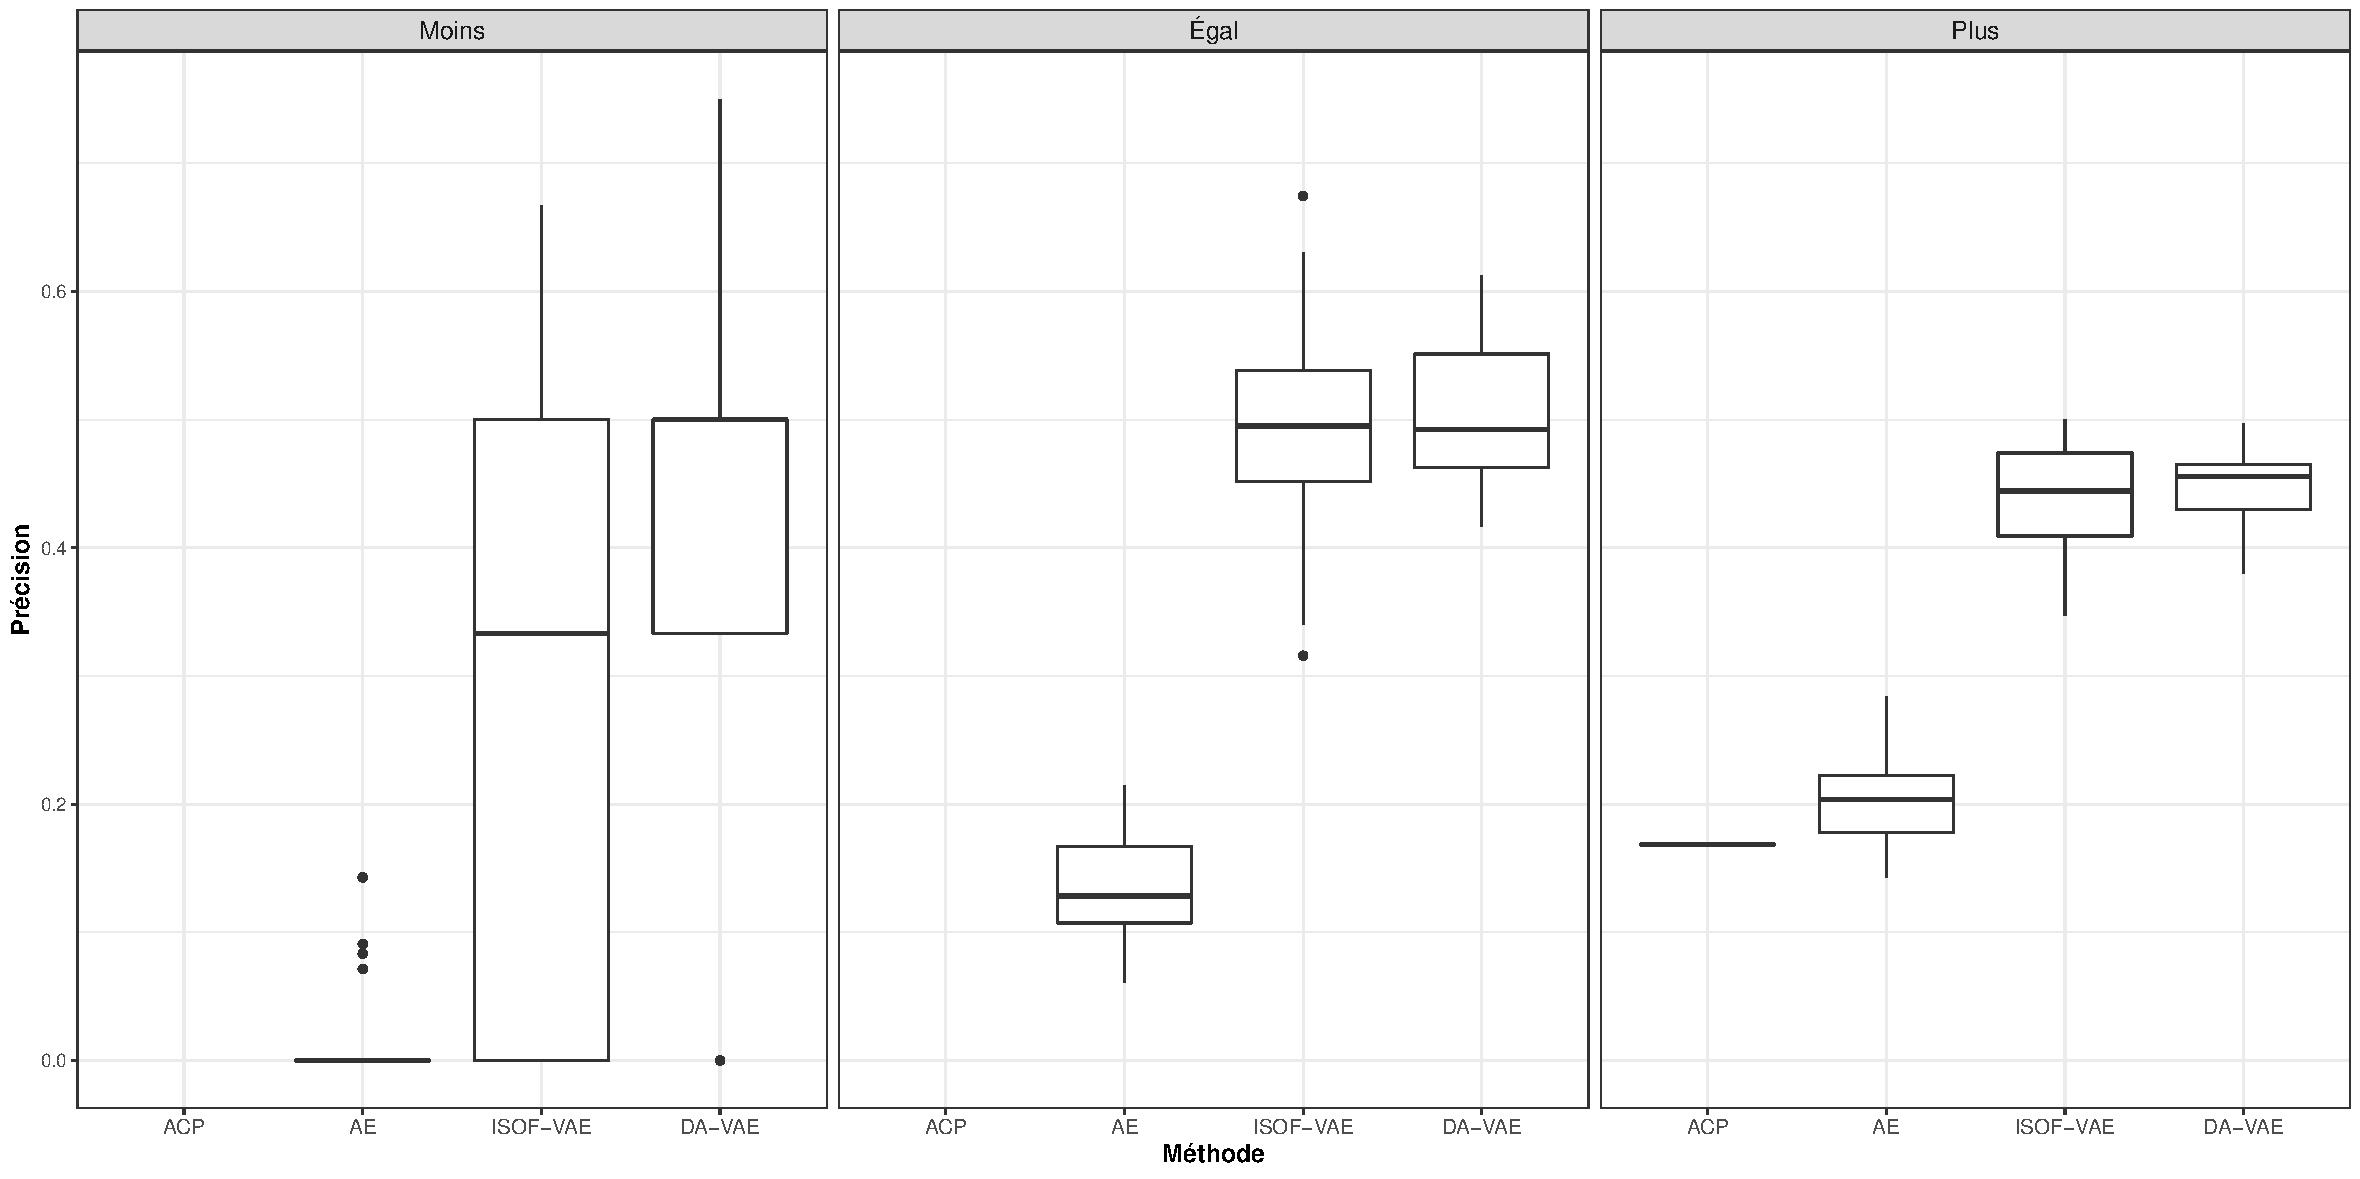
\includegraphics[width=12cm]{images/images_boxplots/precision_cars.pdf}
		\caption{Résultats en précision}
	\end{subfigure}
	\begin{subfigure}{12cm}
		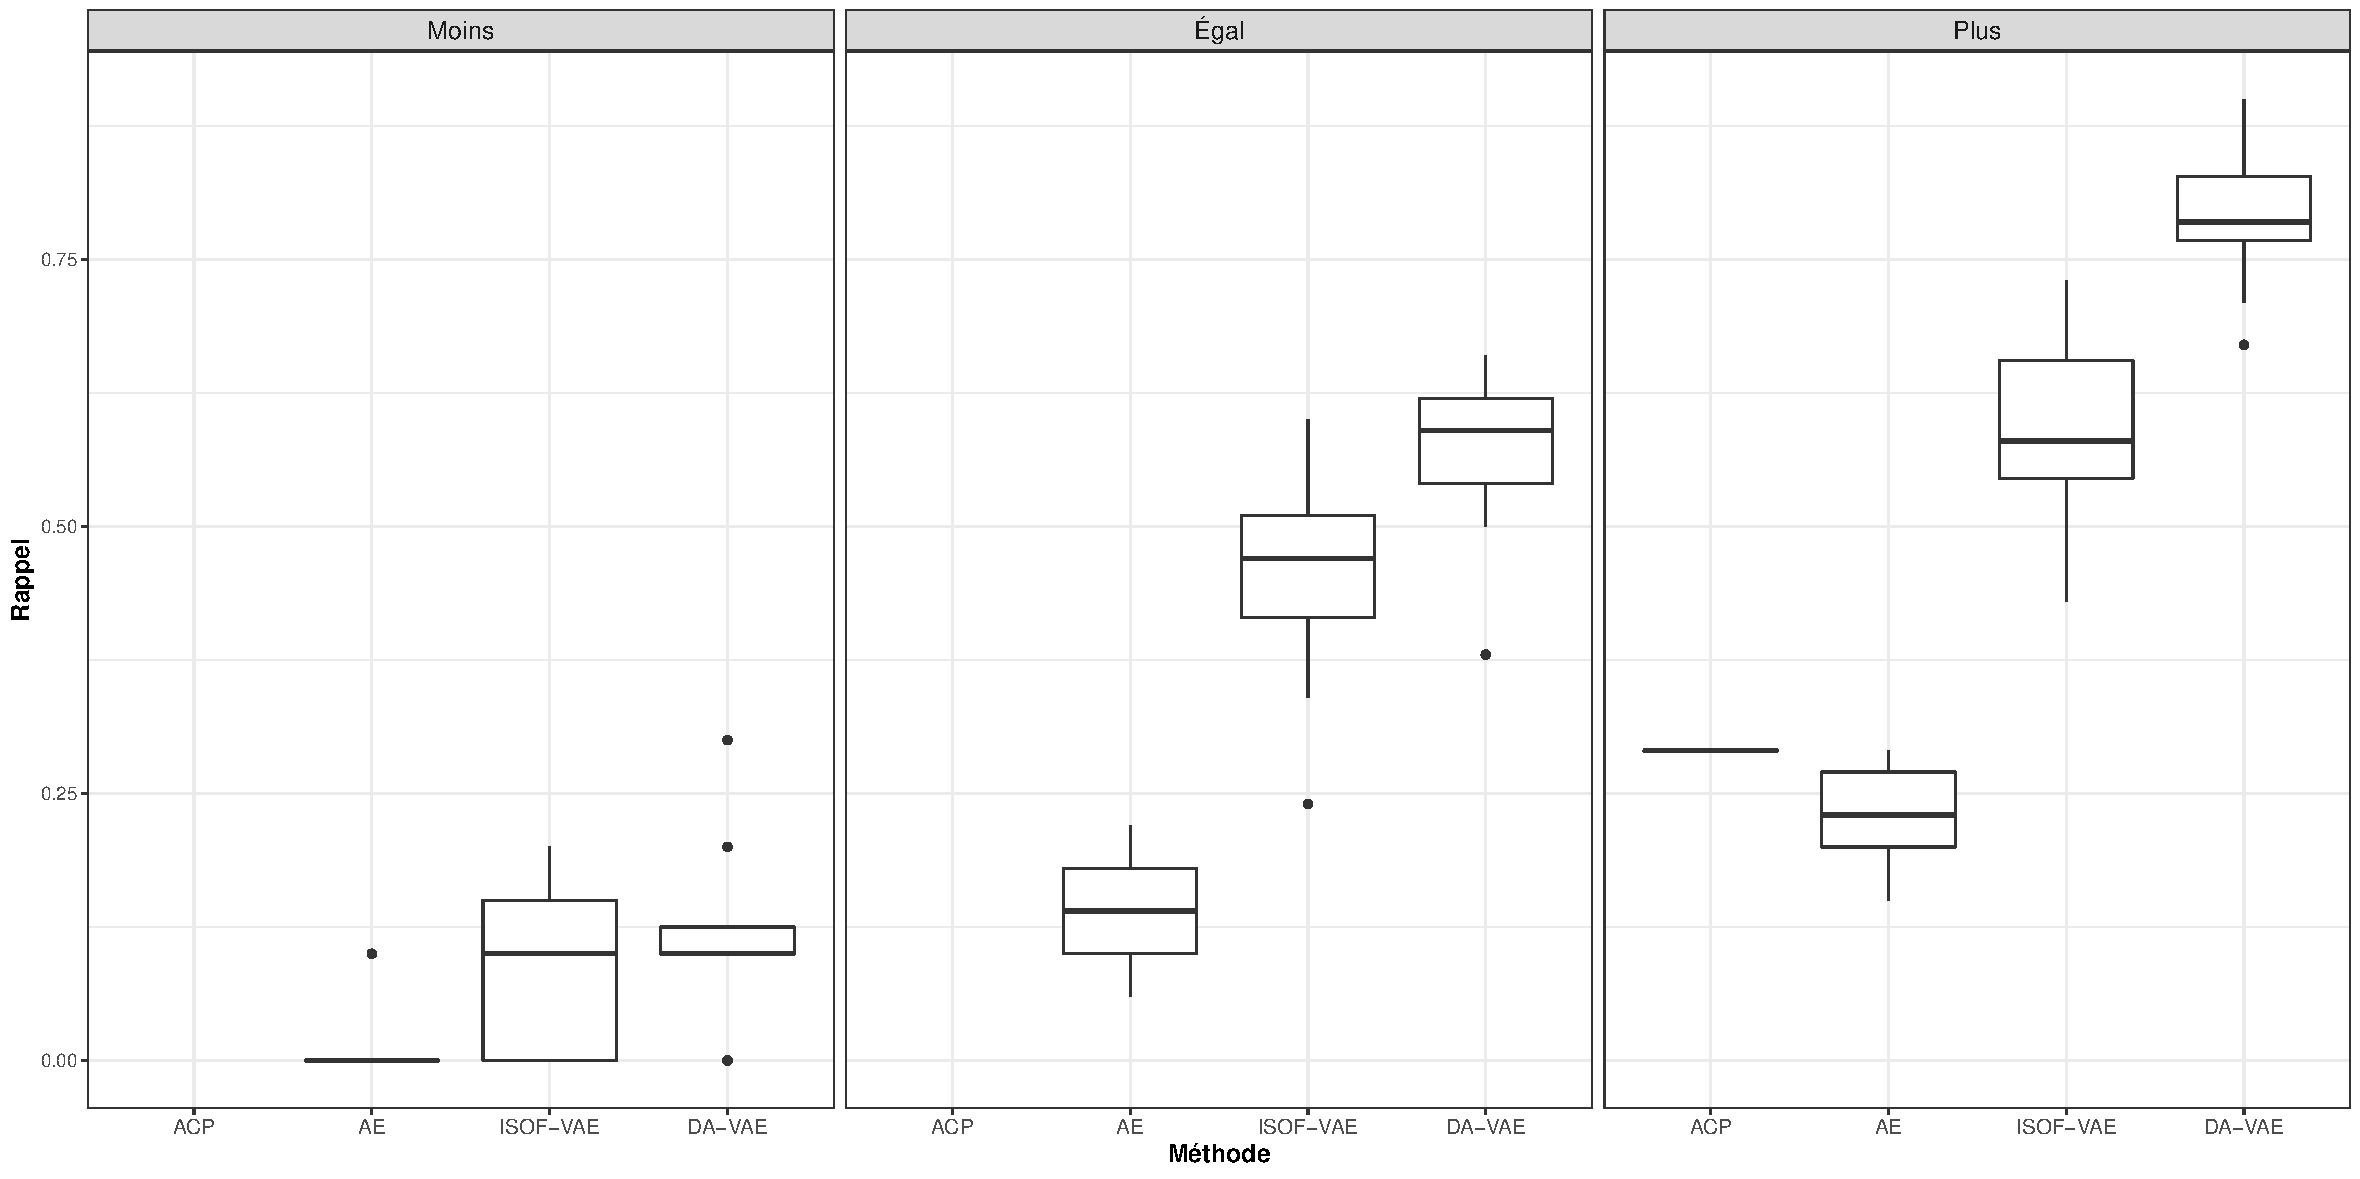
\includegraphics[width=12cm]{images/images_boxplots/recall_cars.pdf}
		\caption{Résultats en rappel}
	\end{subfigure}
	\caption{Graphiques en boîtes et moustaches illustrant les résultats sur les 20 expérimentations de chacune des approches et scénarios de contamination. Les 3 sous-figures concernent une métrique différente.}
	\label{fig:auc_cars}
\end{figure}

\subsection{MNIST}

Le tableau \ref{tab:auc_mnist} synthétise les résultats obtenus sur le jeu de données \textit{MNIST} pour la métrique d'aire sous la courbe ROC. Les résultats sont présentés par scénario de contamination et par scénario de test (voir tableau \ref{tab:mnist_scenarios} pour plus de détails sur les scénarios de test). Les résultats pour les métriques de précision et de rappel sont présentés de la même manière dans les tableaux \ref{tab:precision_mnist} et \ref{tab:recall_mnist} respectivement. Nous avons mis en gras les résultats de la méthode nous apparaissant la plus adaptée pour chacun des scénarios. Encore une fois, ce choix est basé en grande partie sur la valeur moyenne de la métrique.

\begin{table}[h]
	\centering
	\caption{Résultats des aires sous la courbe ROC des différentes approches selon le scénario de contamination et le scénario de test appliqué sur le jeu de données \textit{MNIST}.}
	\begin{tabular}{c|c|c c c c}
		\toprule
		Contamination & Scénario & ACP & AE & ISOF-VAE & DA-VAE \\
		\hline
		\multirow{6}{*}{Moins} 
		& 1 & $\mathbf{0.991 \pm 0.006}$ & 0.990 $\pm$ 0.004 & $0.969 \pm 0.031$ & 0.987 $\pm$ 0.007   \\
		& 2 & $\mathbf{0.988 \pm 0.005}$ & $\mathbf{0.988 \pm 0.005}$ & $0.965 \pm 0.022$ & 0.982 $\pm$ 0.021   \\
		& 3 & 0.993 $\pm$ 0.005 & $\mathbf{0.994 \pm 0.004}$ & $0.976 \pm 0.017$ & 0.992 $\pm$ 0.005   \\
		& 4 & 0.893 $\pm$ 0.034 & $\mathbf{0.929 \pm 0.034}$ & $0.754 \pm 0.078$ & 0.836 $\pm$ 0.067   \\			
		& 5 & 0.893 $\pm$ 0.035 & $\mathbf{0.948 \pm 0.026}$ & $0.794 \pm 0.061$ & 0.880 $\pm$ 0.059   \\
		& 6 & 0.856 $\pm$ 0.059 & 0.847 $\pm$ 0.092 & $0.850 \pm 0.065$ & $\mathbf{0.893 \pm 0.046}$   \\
		\midrule
		\multirow{6}{*}{Égal} 
		& 1 & 0.993 $\pm$ 0.004 & $\mathbf{0.994 \pm 0.002}$ & $0.980 \pm 0.011$ & $\mathbf{0.994 \pm 0.002}$   \\
		& 2 & 0.991 $\pm$ 0.003 & $\mathbf{0.992 \pm 0.002}$ & $0.978 \pm 0.010$ & 0.988 $\pm$ 0.007   \\
		& 3 & 0.993 $\pm$ 0.004 & $\mathbf{0.996 \pm 0.001}$ & $0.980 \pm 0.011$ & 0.991 $\pm$ 0.007   \\
		& 4 & 0.903 $\pm$ 0.027 & $\mathbf{0.959 \pm 0.012}$ & $0.828 \pm 0.060$ & 0.901 $\pm$ 0.042   \\			
		& 5 & 0.913 $\pm$ 0.027 & $\mathbf{0.969 \pm 0.010}$ & $0.824 \pm 0.057$ & 0.871 $\pm$ 0.122   \\
		& 6 & 0.900 $\pm$ 0.031 & 0.854 $\pm$ 0.049 & $0.860 \pm 0.056$ & $\mathbf{0.921 \pm 0.036}$   \\
		\midrule
		\multirow{6}{*}{Plus} 
		& 1 & 0.994 $\pm$ 0.003 & $\mathbf{0.998 \pm 0.001}$ & $0.986 \pm 0.009$ & 0.994 $\pm$ 0.003   \\
		& 2 & 0.993 $\pm$ 0.004 & $\mathbf{0.997 \pm 0.001}$ & $0.981 \pm 0.009$ & 0.991 $\pm$ 0.007   \\
		& 3 & 0.993 $\pm$ 0.003 & $\mathbf{0.998 \pm 0.001}$ & $0.985 \pm 0.008$ & 0.995 $\pm$ 0.002   \\
		& 4 & 0.942 $\pm$ 0.025 & $\mathbf{0.985 \pm 0.005}$ & $0.833 \pm 0.058$ & 0.915 $\pm$ 0.041   \\			
		& 5 & 0.948 $\pm$ 0.021 & $\mathbf{0.992 \pm 0.003}$ & $0.875 \pm 0.040$ & 0.936 $\pm$ 0.028   \\
		& 6 & 0.929 $\pm$ 0.015 & 0.911 $\pm$ 0.027 & $0.882 \pm 0.031$ & $\mathbf{0.933 \pm 0.028}$   \\
		\midrule
	\end{tabular} 
	\label{tab:auc_mnist}
\end{table}

Dans les figures \ref{fig:auc_mnist}, \ref{fig:precision_mnist} et \ref{fig:recall_mnist}, on peut voir plus en détails la distribution des résultats obtenus pour les 3 différentes métriques sur les 20 expérimentations grâce à des graphiques en boîtes et moustaches.

\begin{figure}[H]
	\centering
	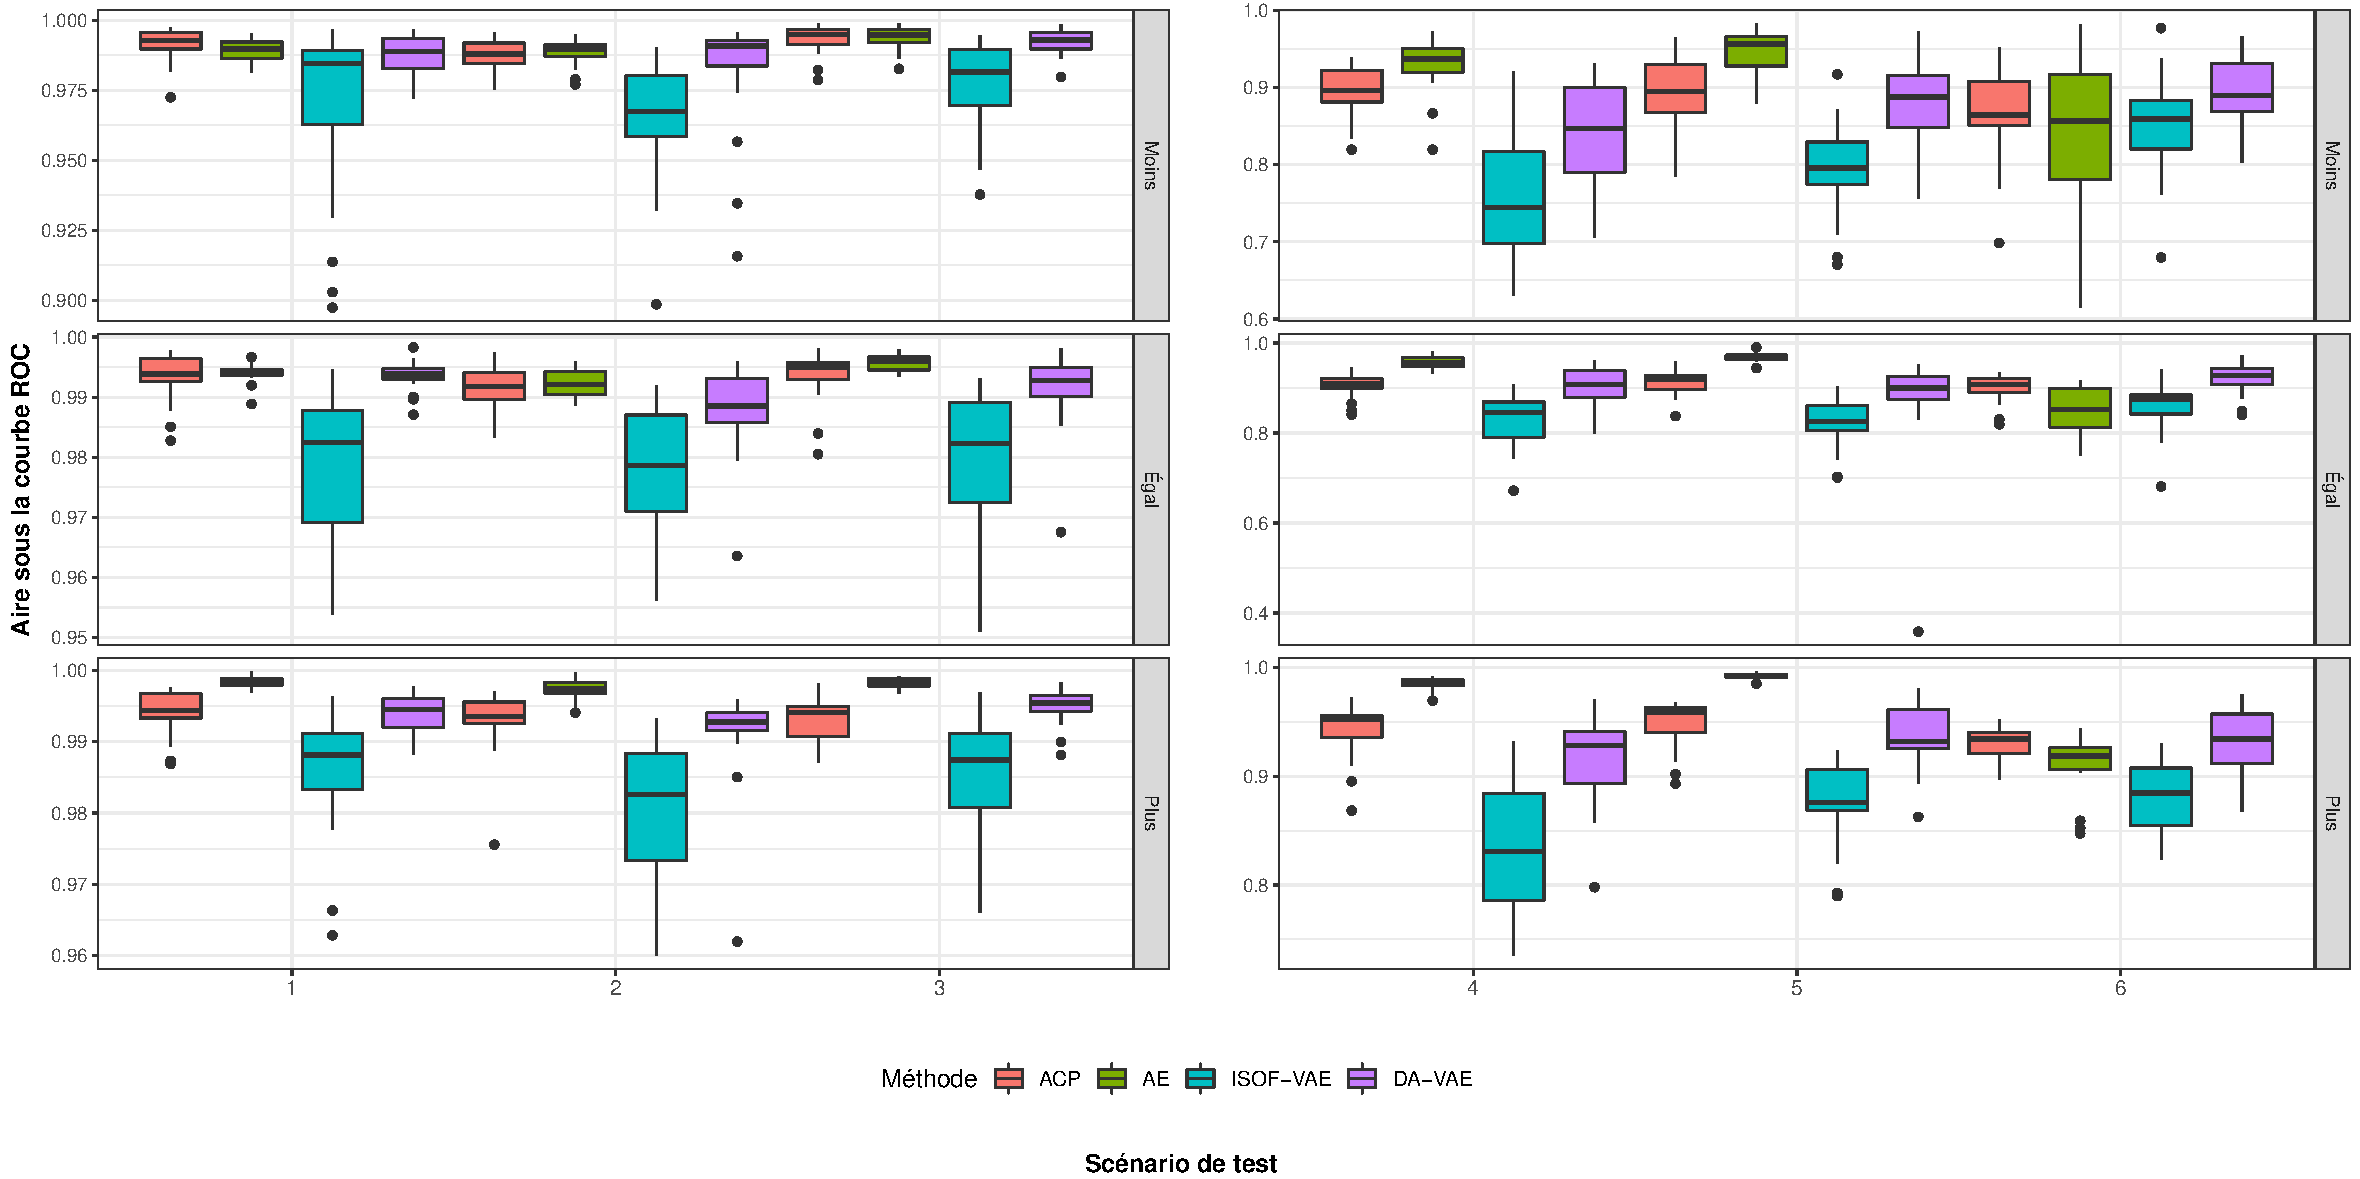
\includegraphics[width=\linewidth]{images/images_boxplots/auc_mnist.pdf}
	\caption{Graphiques en boîtes et moustaches illustrant les résultats sur les 20 expérimentations de chacune des approches, des scénarios de test et des scénarios de contamination. Toutes les figures présentent les résultats en aire sous la courbe ROC.}
	\label{fig:auc_mnist}
\end{figure}

\begin{table}[h]
	\centering
	\caption{Résultats des précisions selon la quantité de contamination et le scénario de test sur le jeu de données \textit{MNIST}. La valeur de $\alpha$ dépend du scénario de contamination. Pour le scénario "Moins" $\alpha=0.01$, pour le scénario "Égal" $\alpha=0.05$ et finalement pour le scénario "Plus" $\alpha=0.1$.}
	\begin{tabular}{c|c|c c c c }
		\toprule
		Contamination & Scénario & ACP & AE & ISOF-VAE & DA-VAE  \\
		\hline
		\multirow{6}{*}{Moins} 
		& 1 & $\mathbf{0.688 \pm 0.384}$ & 0.256 $\pm$ 0.097 & 0.280 $\pm$ 0.255 & 0.271 $\pm$ 0.212  \\
		& 2 & $\mathbf{0.500 \pm 0.424}$ & 0.141 $\pm$ 0.178 & 0.238 $\pm$ 0.234 & 0.282 $\pm$ 0.243  \\
		& 3 & $\mathbf{0.583 \pm 0.482}$ & 0.411 $\pm$ 0.319 & 0.263 $\pm$ 0.289 & 0.387 $\pm$ 0.273  \\
		& 4 & 0.135 $\pm$ 0.182 & $\mathbf{0.197 \pm 0.193}$ & 0.033 $\pm$ 0.057 & 0.020 $\pm$ 0.051  \\			
		& 5 & 0.110 $\pm$ 0.188 & $\mathbf{0.168 \pm 0.212}$ & 0.028 $\pm$ 0.053 & 0.145 $\pm$ 0.159  \\
		& 6 & 0.118 $\pm$ 0.145 & $\mathbf{0.363 \pm 0.267}$ & 0.060 $\pm$ 0.092 & 0.115 $\pm$ 0.142  \\
		\midrule
		\multirow{6}{*}{Égal} 
		& 1 & 0.779 $\pm$ 0.079 & 0.777 $\pm$ 0.037 & 0.678 $\pm$ 0.102 & $\mathbf{0.809 \pm 0.057}$  \\
		& 2 & $\mathbf{0.685 \pm 0.013}$ & 0.672 $\pm$ 0.014 & 0.677 $\pm$ 0.011 & 0.681 $\pm$ 0.009  \\
		& 3 & 0.821 $\pm$ 0.056 & 0.793 $\pm$ 0.033 & 0.702 $\pm$ 0.089 & $\mathbf{0.829 \pm 0.059}$  \\
		& 4 & 0.276 $\pm$ 0.078 & $\mathbf{0.526 \pm 0.063}$ & 0.216 $\pm$ 0.096 & 0.375 $\pm$ 0.108  \\			
		& 5 & 0.329 $\pm$ 0.081 & $\mathbf{0.556 \pm 0.050}$ & 0.210 $\pm$ 0.097 & 0.358 $\pm$ 0.104  \\
		& 6 & 0.331 $\pm$ 0.065 & $\mathbf{0.501 \pm 0.056}$ & 0.283 $\pm$ 0.094 & 0.443 $\pm$ 0.113  \\
		\midrule
		\multirow{6}{*}{Plus} 
		& 1 & 0.535 $\pm$ 0.016 & $\mathbf{0.563 \pm 0.020}$ & 0.545 $\pm$ 0.021 & 0.555 $\pm$ 0.027  \\
		& 2 & $\mathbf{0.583 \pm 0.024}$ & 0.566 $\pm$ 0.021 & 0.550 $\pm$ 0.036 & 0.556 $\pm$ 0.025  \\
		& 3 & 0.531 $\pm$ 0.025 & $\mathbf{0.571 \pm 0.016}$ & 0.540 $\pm$ 0.025 & 0.559 $\pm$ 0.018  \\
		& 4 & 0.455 $\pm$ 0.048 & $\mathbf{0.496 \pm 0.020}$ & 0.321 $\pm$ 0.083 & 0.424 $\pm$ 0.057  \\			
		& 5 & 0.452 $\pm$ 0.039 & $\mathbf{0.507 \pm 0.020}$ & 0.379 $\pm$ 0.061 & 0.452 $\pm$ 0.050  \\
		& 6 & 0.425 $\pm$ 0.023 & $\mathbf{0.464 \pm 0.022}$ & 0.394 $\pm$ 0.044 & 0.456 $\pm$ 0.036  \\
		\midrule
	\end{tabular} 
	\label{tab:precision_mnist}
\end{table}

\begin{figure}[H]
	\centering
	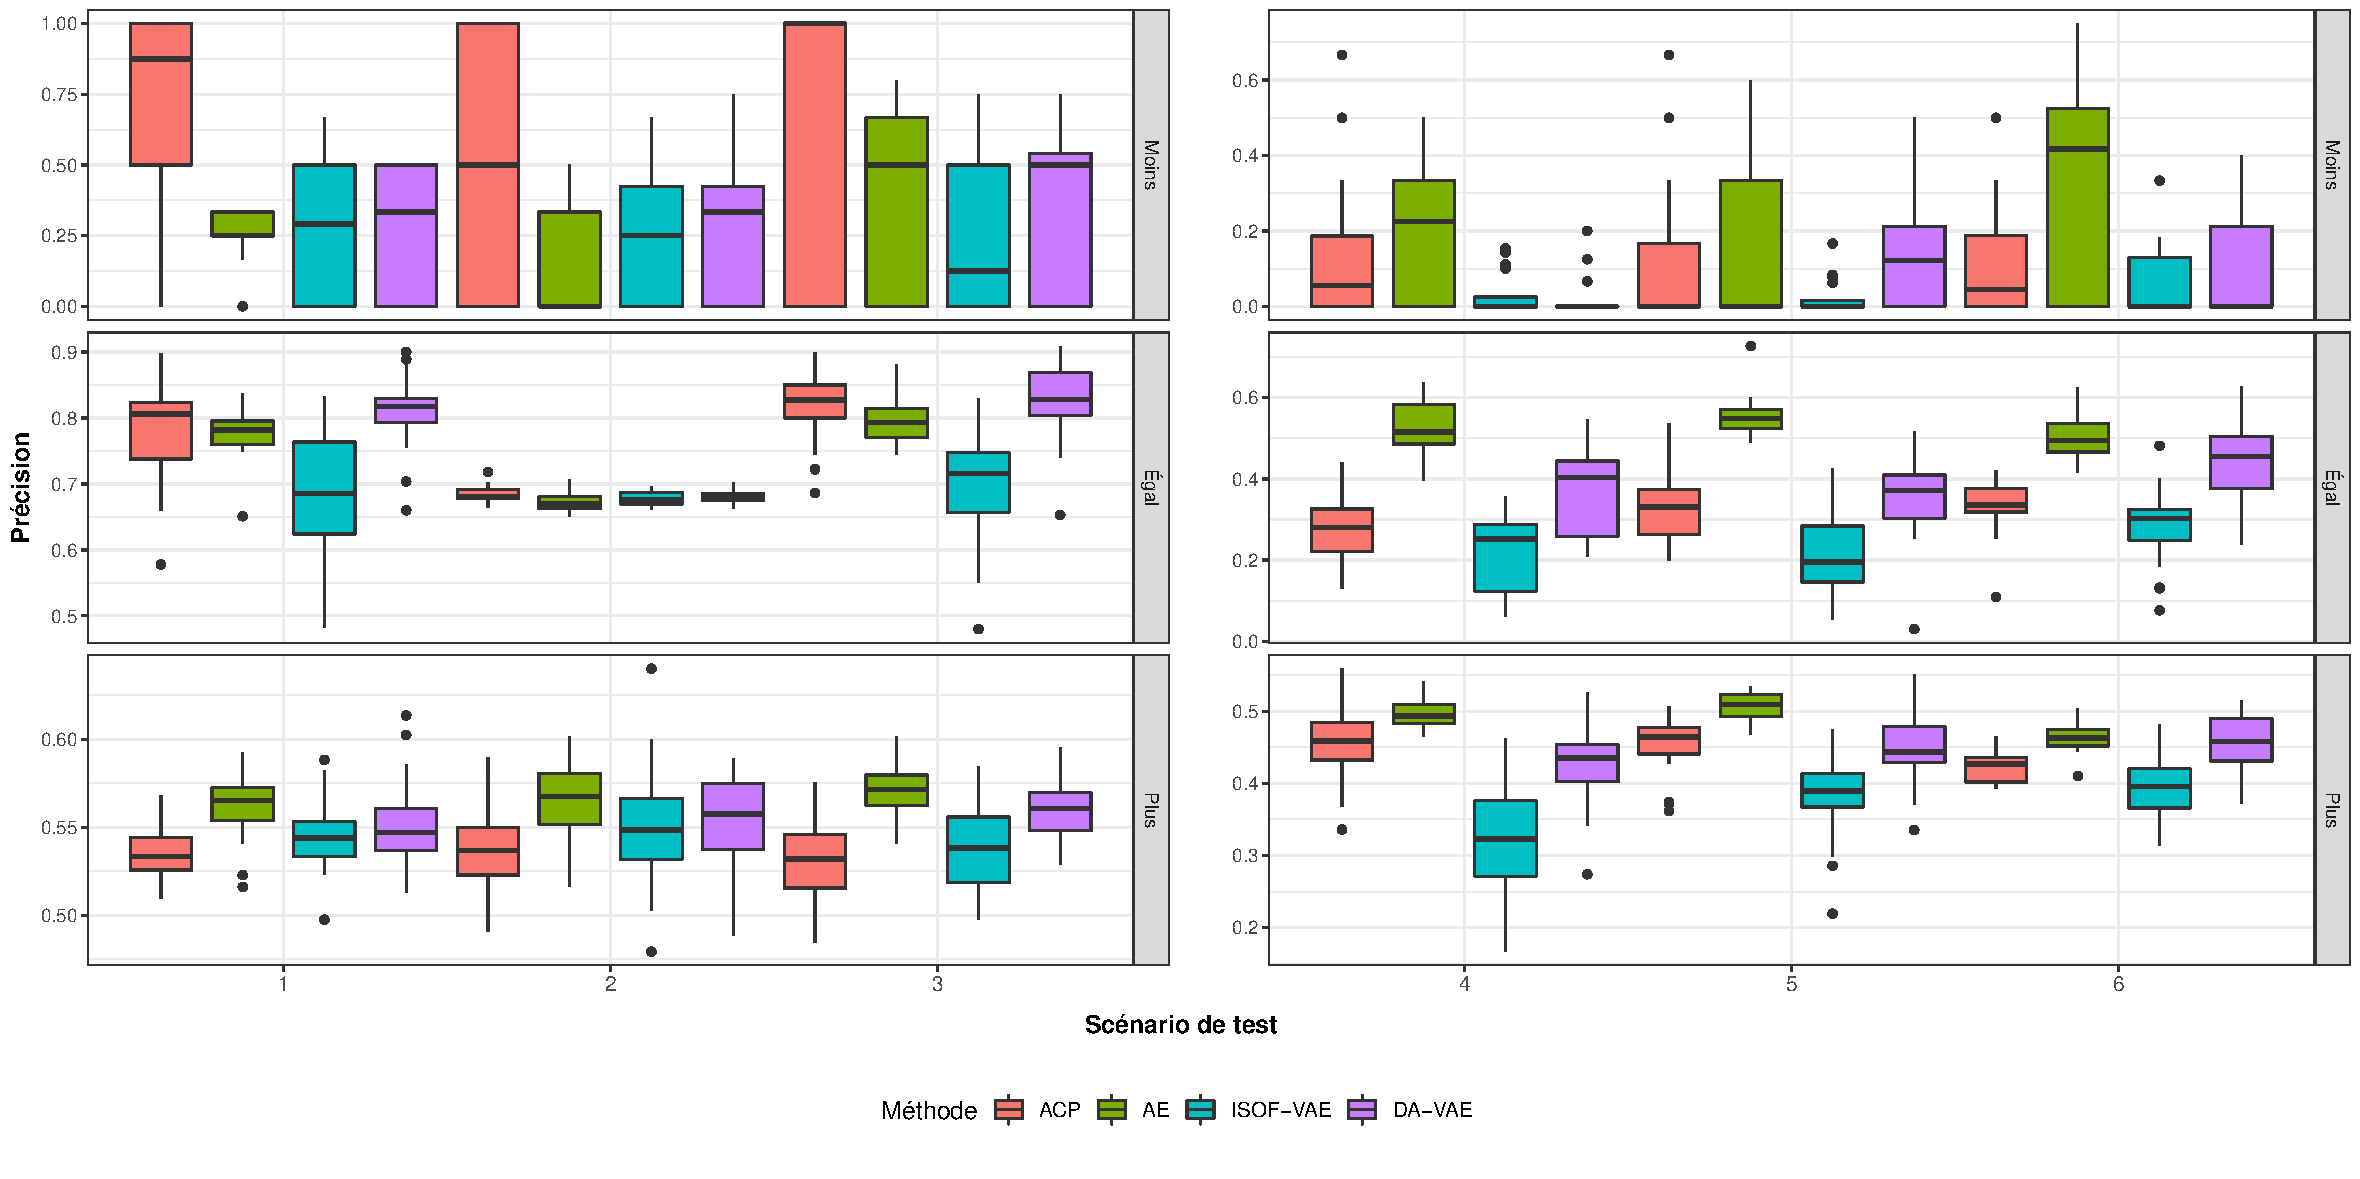
\includegraphics[width=\linewidth]{images/images_boxplots/precision_mnist.pdf}
	\caption{Graphiques en boîtes et moustaches illustrant les résultats sur les 20 expérimentations de chacune des approches, des scénarios de test et des scénarios de contamination. Toutes les figures présentent les résultats en précision.}
	\label{fig:precision_mnist}
\end{figure}

\begin{table}[h]
	\centering
	\caption{Résultats des rappels selon la quantité de contamination et le scénario de test sur le jeu de données \textit{MNIST}. La valeur de $\alpha$ dépend du scénario de contamination. Pour le scénario "Moins" $\alpha=0.01$, pour le scénario "Égal" $\alpha=0.05$ et finalement pour le scénario "Plus" $\alpha=0.1$.}
	\begin{tabular}{c|c|c c c c }
		\toprule
		Contamination & Scénario & ACP & AE & ISOF-VAE & DA-VAE  \\
		\hline
		\multirow{6}{*}{Moins} 
		& 1 & $\mathbf{0.200 \pm 0.139}$ & 0.138 $\pm$ 0.067 & 0.095 $\pm$ 0.092 & 0.075 $\pm$ 0.062  \\
		& 2 & $\mathbf{0.100 \pm 0.085}$ & 0.081 $\pm$ 0.107 & 0.085 $\pm$ 0.079 & 0.1 $\pm$ 0.095  \\
		& 3 & 0.131 $\pm$ 0.134 & $\mathbf{0.181 \pm 0.170}$ & 0.09 $\pm$ 0.118 & 0.11 $\pm$ 0.094  \\
		& 4 & $\mathbf{0.100 \pm 0.116}$ & 0.088 $\pm$ 0.089 & 0.038 $\pm$ 0.070 & 0.025 $\pm$ 0.063  \\			
		& 5 & 0.063 $\pm$ 0.093 & 0.075 $\pm$ 0.108 & 0.031 $\pm$ 0.054 & $\mathbf{0.088 \pm 0.089}$  \\
		& 6 & 0.081 $\pm$ 0.099 & $\mathbf{0.156 \pm 0.130}$ & 0.056 $\pm$ 0.084 & 0.0625 $\pm$ 0.074  \\
		\midrule
		\multirow{6}{*}{Égal} 
		& 1 & 0.859 $\pm$ 0.083 & $\mathbf{0.871 \pm 0.067}$ & 0.663 $\pm$ 0.110 & 0.778 $\pm$ 0.066  \\
		& 2 & $\mathbf{1.000 \pm 0.000}$ & $\mathbf{1.000 \pm 0.000}$ & 1.000 $\pm$ 0.001 & 1.000 $\pm$ 0.001  \\
		& 3 & 0.873 $\pm$ 0.079 & $\mathbf{0.901 \pm 0.038}$ & 0.671 $\pm$ 0.116 & 0.786 $\pm$ 0.064  \\
		& 4 & 0.381 $\pm$ 0.096 & $\mathbf{0.628 \pm 0.090}$ & 0.239 $\pm$ 0.110 & 0.412 $\pm$ 0.123  \\			
		& 5 & 0.451 $\pm$ 0.123 & $\mathbf{0.645 \pm 0.079}$ & 0.230 $\pm$ 0.099 & 0.401 $\pm$ 0.112  \\
		& 6 & 0.435 $\pm$ 0.100 & $\mathbf{0.588 \pm 0.076}$ & 0.319 $\pm$ 0.101 & 0.481 $\pm$ 0.120  \\
		\midrule
		\multirow{6}{*}{Plus} 
		& 1 & 0.997 $\pm$ 0.005 & $\mathbf{1.000 \pm 0.000}$ & 0.980 $\pm$ 0.028 & 0.995 $\pm$ 0.007  \\
		& 2 & 0.994 $\pm$ 0.011 & $\mathbf{1.000 \pm 0.000}$ & 0.963 $\pm$ 0.031 & 0.985 $\pm$ 0.027  \\
		& 3 & 0.994 $\pm$ 0.008 & $\mathbf{1.000 \pm 0.000}$ & 0.977 $\pm$ 0.023 & 0.996 $\pm$ 0.010  \\
		& 4 & 0.841 $\pm$ 0.085 & $\mathbf{0.984 \pm 0.012}$ & 0.476 $\pm$ 0.159 & 0.733 $\pm$ 0.137  \\			
		& 5 & 0.873 $\pm$ 0.091 & $\mathbf{0.994 \pm 0.007}$ & 0.593 $\pm$ 0.139 & 0.824 $\pm$ 0.102  \\
		& 6 & 0.789 $\pm$ 0.055 & $\mathbf{0.859 \pm 0.047}$ & 0.629 $\pm$ 0.104 & 0.807 $\pm$ 0.097  \\
		\midrule
	\end{tabular} 
	\label{tab:recall_mnist}
\end{table}

\begin{figure}[H]
	\centering
	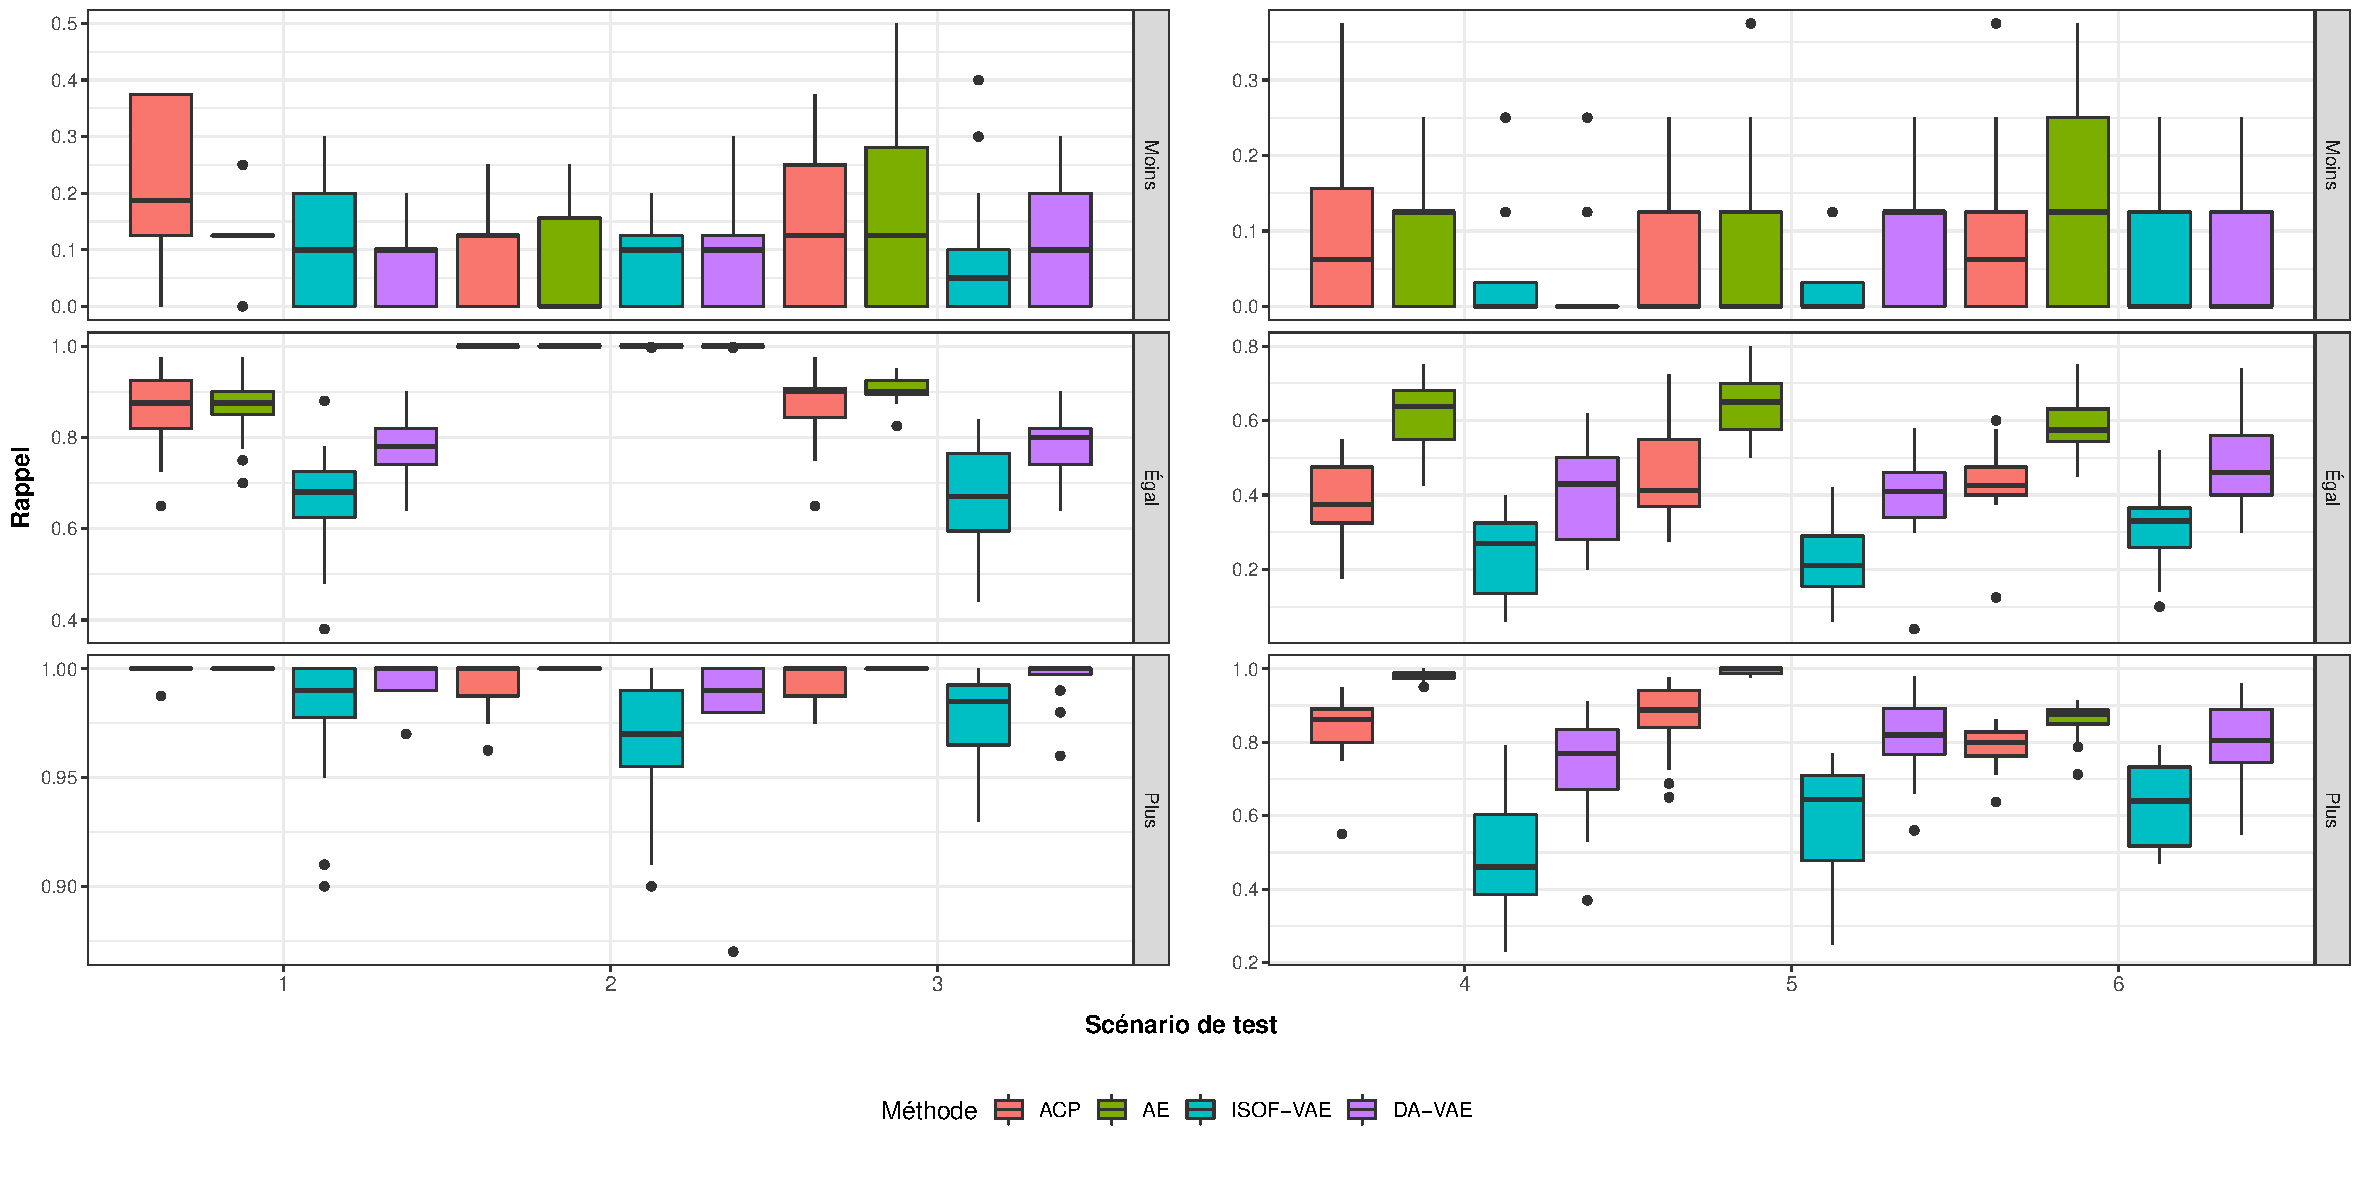
\includegraphics[width=\linewidth]{images/images_boxplots/recall_mnist.pdf}
	\caption{Graphiques en boîtes et moustaches illustrant les résultats sur les 20 expérimentations de chacune des approches, des scénarios de test et des scénarios de contamination. Toutes les figures présentent les résultats en rappel.}
	\label{fig:recall_mnist}
\end{figure}

\section{Discussion} \label{discussion}

Dans les prochaines sous-sections, nous discuterons des résultats obtenus par les différentes méthodes sur les deux jeux de données. Nous irons également plus en profondeur dans l'analyse de la méthode DA-VAE en regardant le comportement de la perte en entraînement ainsi que la composition des représentations latentes produites par le modèle. Finalement, nous étudierons l'impact du niveau de contamination sur les résultats et la pertinence du niveau de filtration $\alpha$.

\subsection{Résultats sur \textit{ImageNet}} \label{imagenet_results}

Dans le tableau \ref{tab:results_cars}, on peut voir les performances en aire sous la courbe ROC, en précision et en rappel de chacune des approches. Pour les 3 scénarios de contamination différents, on remarque que 2 méthodes sont beaucoup plus performantes, et ce, pour les 3 métriques. Ces 2 approches sont: ISOF-VAE et DA-VAE. Il est intéressant de remarquer que ces 2 approches utilisent la représentation latente de l'image pour discriminer les anomalies des observations "normales" plutôt que la reconstruction faite sur les dimensions originales de l'image. Dans le cas spécifique avec les données de \textit{ImageNet}, les images sont de dimensions $128 \times 128 \times 3$, ce qui veut dire que la discrimination des méthodes ACP et AE est basée sur un vecteur de longueur 49 152. À l'inverse, les méthodes ISOF-VAE et DA-VAE utilisent plutôt les vecteurs $\mathbf{\mu}$ et $\mathbf{\sigma}$, chacun de longueur 25. Dans la sous-section \ref{imagenet:reconsruction}, nous ferons l'analyse plus en profondeur des résultats moins performants des méthodes basées sur la reconstruction.

Notre approche DA-VAE est celle qui est la plus performante selon les métriques moyennes analysées. En tenant compte de la variabilité, il n'est cependant pas toujours possible d'affirmer que la méthode DA-VAE est significativement supérieure à la méthode ISOF-VAE. Si on ajoute 2 écarts-types aux métriques moyennes obtenues par ISOF-VAE, cette borne supérieure chevauche souvent la borne inférieure de la méthode DA-VAE. On peut toutefois remarquer que les performances en aire sous la courbe ROC de la méthode DA-VAE demeurent élevées, et ce, pour les 3 scénarios de contamination. Dans le cas de ISOF-VAE, les performances moyennes en aire sous la courbe ROC passent de 0.886 pour le scénario "Moins" à 0.811 pour le scénario "Plus". La variabilité des résultats de notre approche DA-VAE est également inférieure à ceux obtenus sur ISOF-VAE pour les trois métriques. En analysant davantage les résultats sur les trois différents scénarios de contamination, on peut remarquer que pour toutes les approches, le scénario de contamination "Moins" est celui qui témoigne de la plus grande volatilité dans ses performances en test. Cela était prévisible sachant qu'il n'y a que très peu d'anomalies, soit $1\%$, dans le jeu de données de test. Dans les 3 sous-figures de la figure \ref{fig:pvalues_scenarios}, on peut voir les scores d'anomalie prédits pour chacune des observations du jeu de données test en fonction de si l'observation est "anormale" ou non, et ce, pour les 3 scénarios de contamination. Chacun des points correspond à une observation. Les observations sont ordonnées en ordre croissant selon l'inverse de leur score d'anomalie, soit $1-\gamma$. Ce score d'anomalie est défini à l'équation \ref{eq:score_anomalie}. Entre d'autres mots, plus une observation est située à gauche sur l'axe des $x$, plus elle est "anormale" selon le modèle DA-VAE. Les points de couleur violette sont des observations que nous connaissons comme "normales" alors que les points jaunes sont des observations que nous connaissons comme "anormales". Le trait horizontal rouge correspond à la valeur de notre niveau de filtration $\alpha$. Avec ce niveau de filtration, les observations sous la droite rouge sont considérées "anormales" alors que celles au-dessus sont considérées comme "normales" selon le modèle. La ligne verte correspond simplement à un trait partant de l'origine $(0,0)$ et allant jusqu'au point $(1,1)$. Cette ligne nous servira de point de référence pour comparer différents scénarios de contamination. Pour chaque sous-figure, nous présentons une vue complète des observations du jeu de données de test ainsi qu'une vue rapprochée sur les observations situées plus à gauche de l'axe des $x$.

\begin{figure}[htb]
	\centering
	\begin{subfigure}{6cm}
		\centering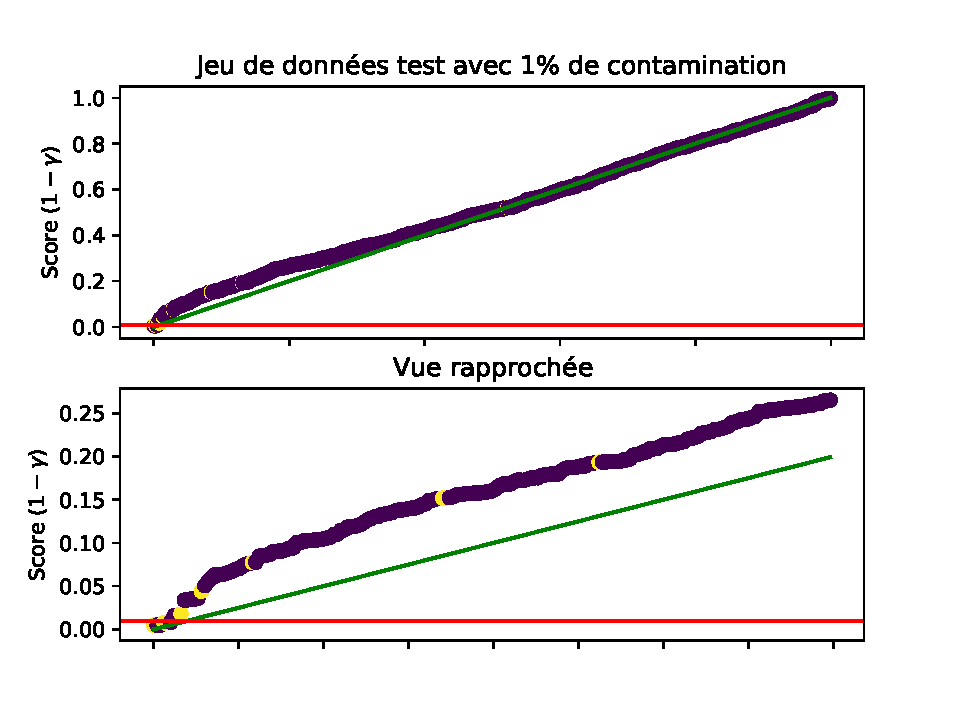
\includegraphics[width=6cm]{images/images_davae/pvalues_scenario_cars_moins}
		\caption{Scénario "Moins"}
	\end{subfigure}
	\begin{subfigure}{6cm}
		\centering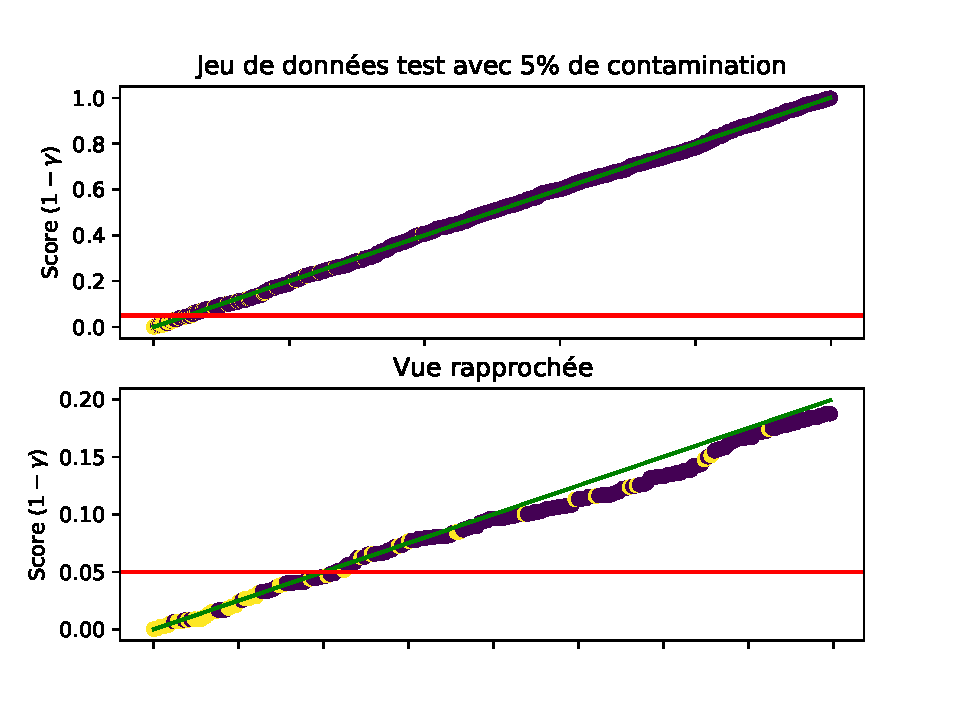
\includegraphics[width=6cm]{images/images_davae/pvalues_scenario_cars_egal}
		\caption{Scénario "Égal"}
	\end{subfigure}
	\begin{subfigure}{6cm}
		\centering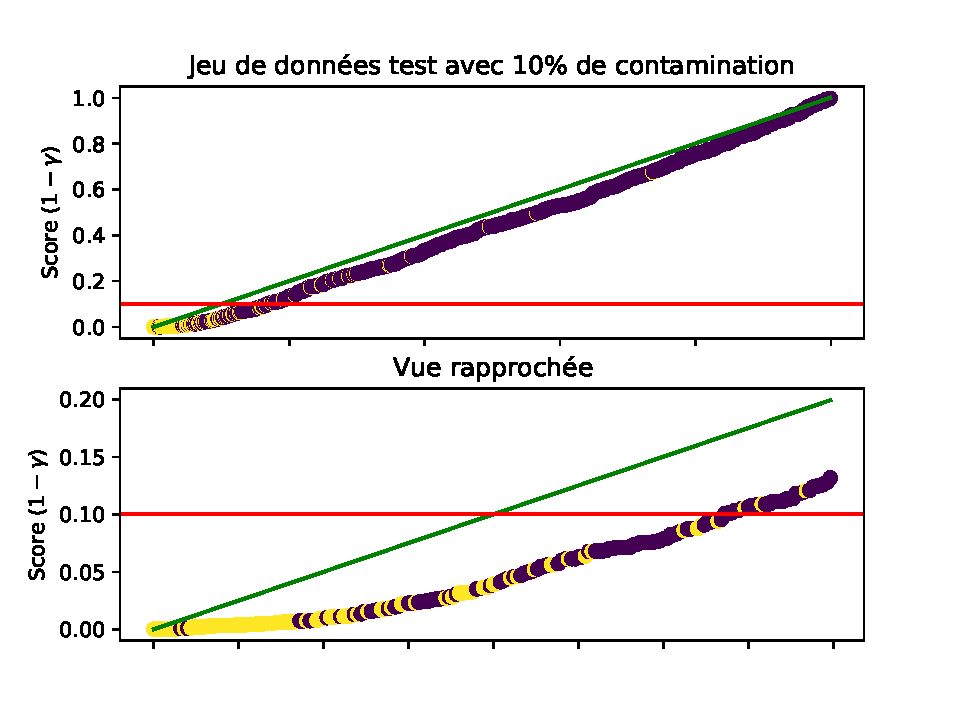
\includegraphics[width=6cm]{images/images_davae/pvalues_scenario_cars_plus}
		\caption{Scénario "Plus"}
	\end{subfigure}
	\caption{Graphiques illustrant les scores d'anomalies selon le scénario de contamination pour le modèle DA-VAE appliqué sur le jeu de données \textit{ImageNet}. Les points violets sont des observations que nous connaissons comme "normales" alors que les points jaunes sont des observations que nous connaissons comme "anormales". Dans tous les cas, le niveau de filtration $\alpha$ est défini comme le niveau de contamination dans le jeu de données de test. Pour chaque sous-figure, nous présentons une vue complète des observations du jeu de données de test ainsi qu'une vue rapprochée sur les observations situées plus à gauche de l'axe des $x$.} 
	\label{fig:pvalues_scenarios}
\end{figure}

Dans les 3 sous-figures à la figure \ref{fig:pvalues_scenarios}, on peut voir que les observations "anormales", soit les points jaunes, sont principalement regroupées à gauche de l'axe des $x$, ce qui est le comportement souhaité. De plus, on peut remarquer que dans les 3 différents scénarios, les points les plus gauches ne se retrouvent pas à la même position par rapport à la droite verte. Dans le scénario "Égal", l'ensemble des points est relativement bien aligné avec la courbe verte. Cette observation peut s'expliquer par le fait que les deux ensembles de données, $\mathcal{X}$ et $\mathcal{X^*}$, possèdent la même composition en termes de proportion d'anomalies. Dans le scénario "Moins", on peut observer une masse plus importante de points au-dessus de la courbe verte dans les premières observations. Cela est dû au fait que l'ensemble de test possède moins d'anomalies que l'ensemble d'entraînement, ce qui fait en sorte que davantage d'observations obtiennent des scores d'anomalie plus faibles. Finalement, dans le scénario "Plus", on observe qu'une masse de points se situent sous la courbe verte dans les premières observations. À l'inverse du scénario "Moins", l'ensemble de test possède ici davantage d'anomalies, en proportion, que l'ensemble d'entraînement, ce qui fait en sorte que davantage d'observations obtiennent des scores d'anomalies élevées. Cette analyse nous permet de valider visuellement que l'approche s'adapte bien à différentes proportions de contamination dans les jeux de données de test et d'entraînement.

\subsubsection{Analyses des méthodes basées sur la reconstruction} \label{imagenet:reconsruction}

Dans la sous-section précédente, nous avons mentionné que les approches basées sur la reconstruction, soit ACP et AE, sont beaucoup moins performantes que les deux autres approches. D'ailleurs, on remarque que la méthode ACP obtient des aires sous la courbe ROC sous 0.5 pour tous les scénarios de contamination. En théorie, nous aurions donc pu, pour cette méthode, obtenir de meilleurs résultats en calculant notre score d'anomalie comme l'inverse du score actuel. Actuellement, notre prémisse de base est que les images étant les moins bien reconstruites sont potentiellement des anomalies. À l'inverse, les images les mieux reconstruites sont potentiellement des images "normales". Nous avons fait cette hypothèse puisque les anomalies sont peu fréquentes dans nos jeux de données, ce qui devrait faire en sorte que les paramètres appris par le modèle soit davantage représentés par les images "normales". En analysant les résultats en aire sous la courbe ROC obtenus par l'ACP, nous concluons que c'est plutôt les anomalies qui mieux reconstruites que les images "normales". Pour s'en convaincre, nous avons regardé des exemples d'images les mieux reconstruites sur l'ensemble d'entraînement. On peut voir quelques exemples à la figure \ref{fig:acp_reconstructionsa}. Dans le même ordre d'idées, la figure \ref{fig:acp_reconstructionsb} illustre quelques exemples d'images qui les moins bien reconstruites. 

\begin{figure}[H]
	\centering
	\begin{subfigure}{12cm}
		\centering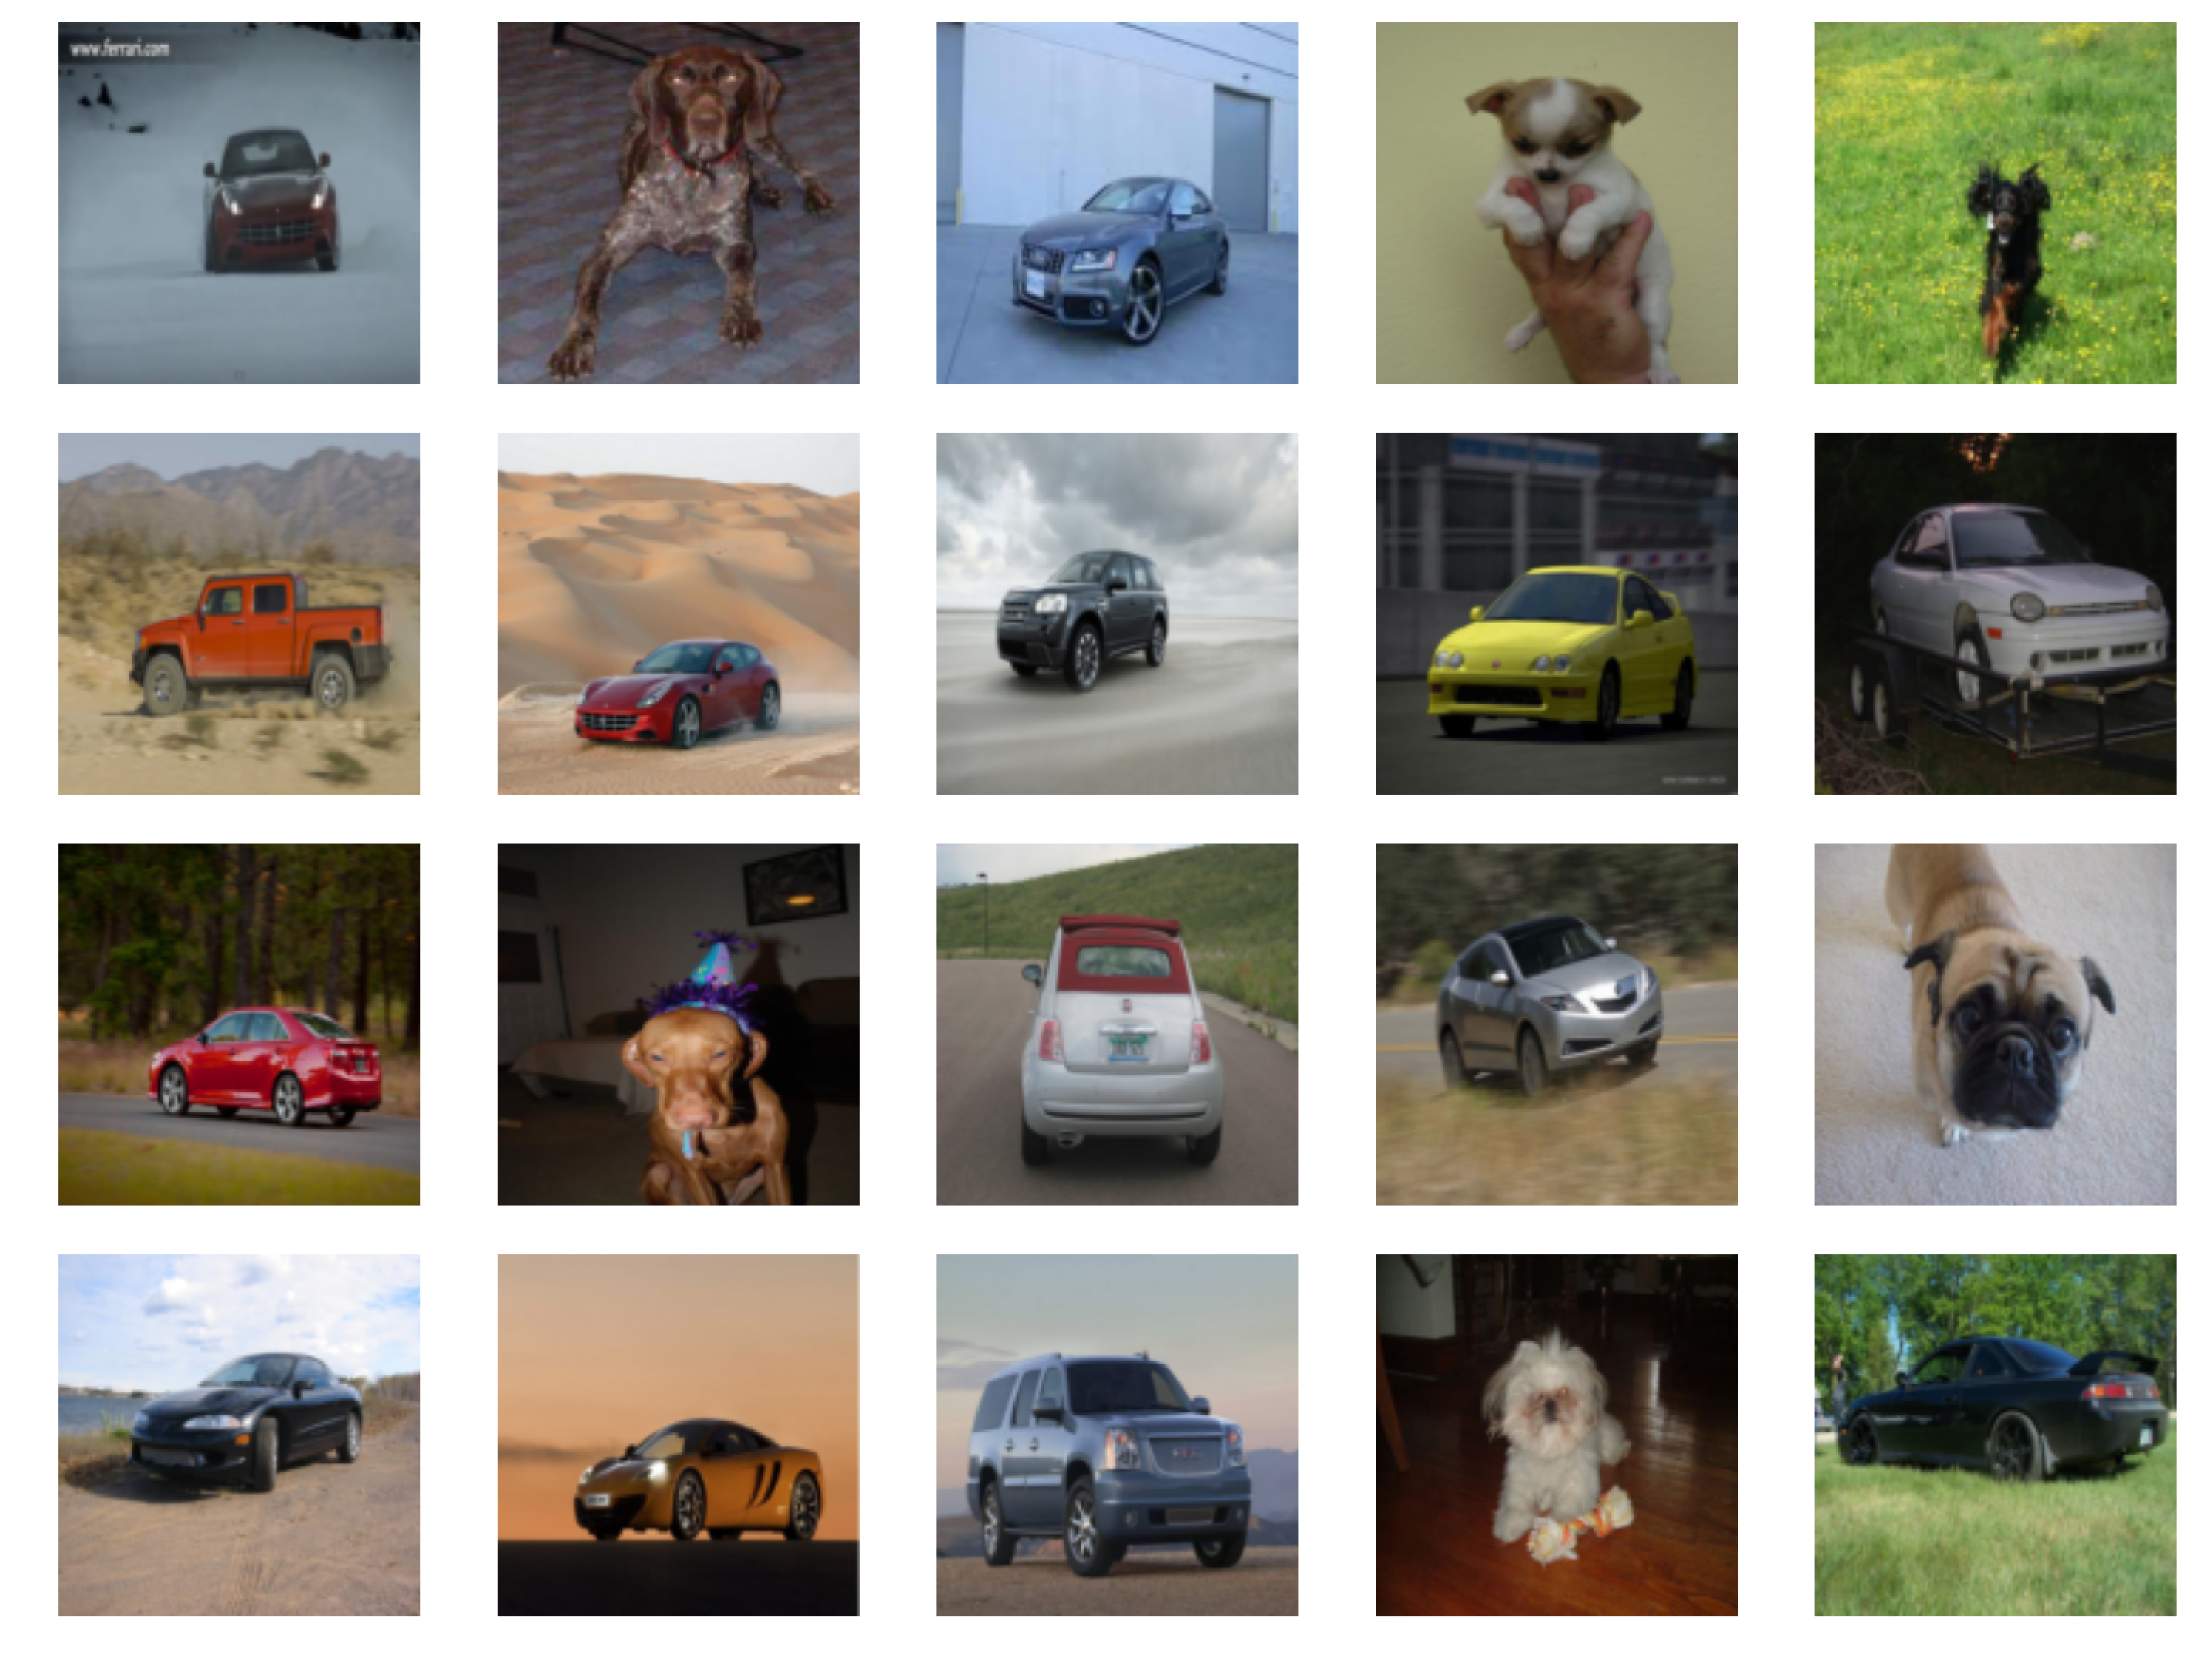
\includegraphics[width=12cm]{images/smallest_errors}
		\caption{Exemples d'images bien reconstruites}
		\label{fig:acp_reconstructionsa}
	\end{subfigure}
	\begin{subfigure}{12cm}
		\centering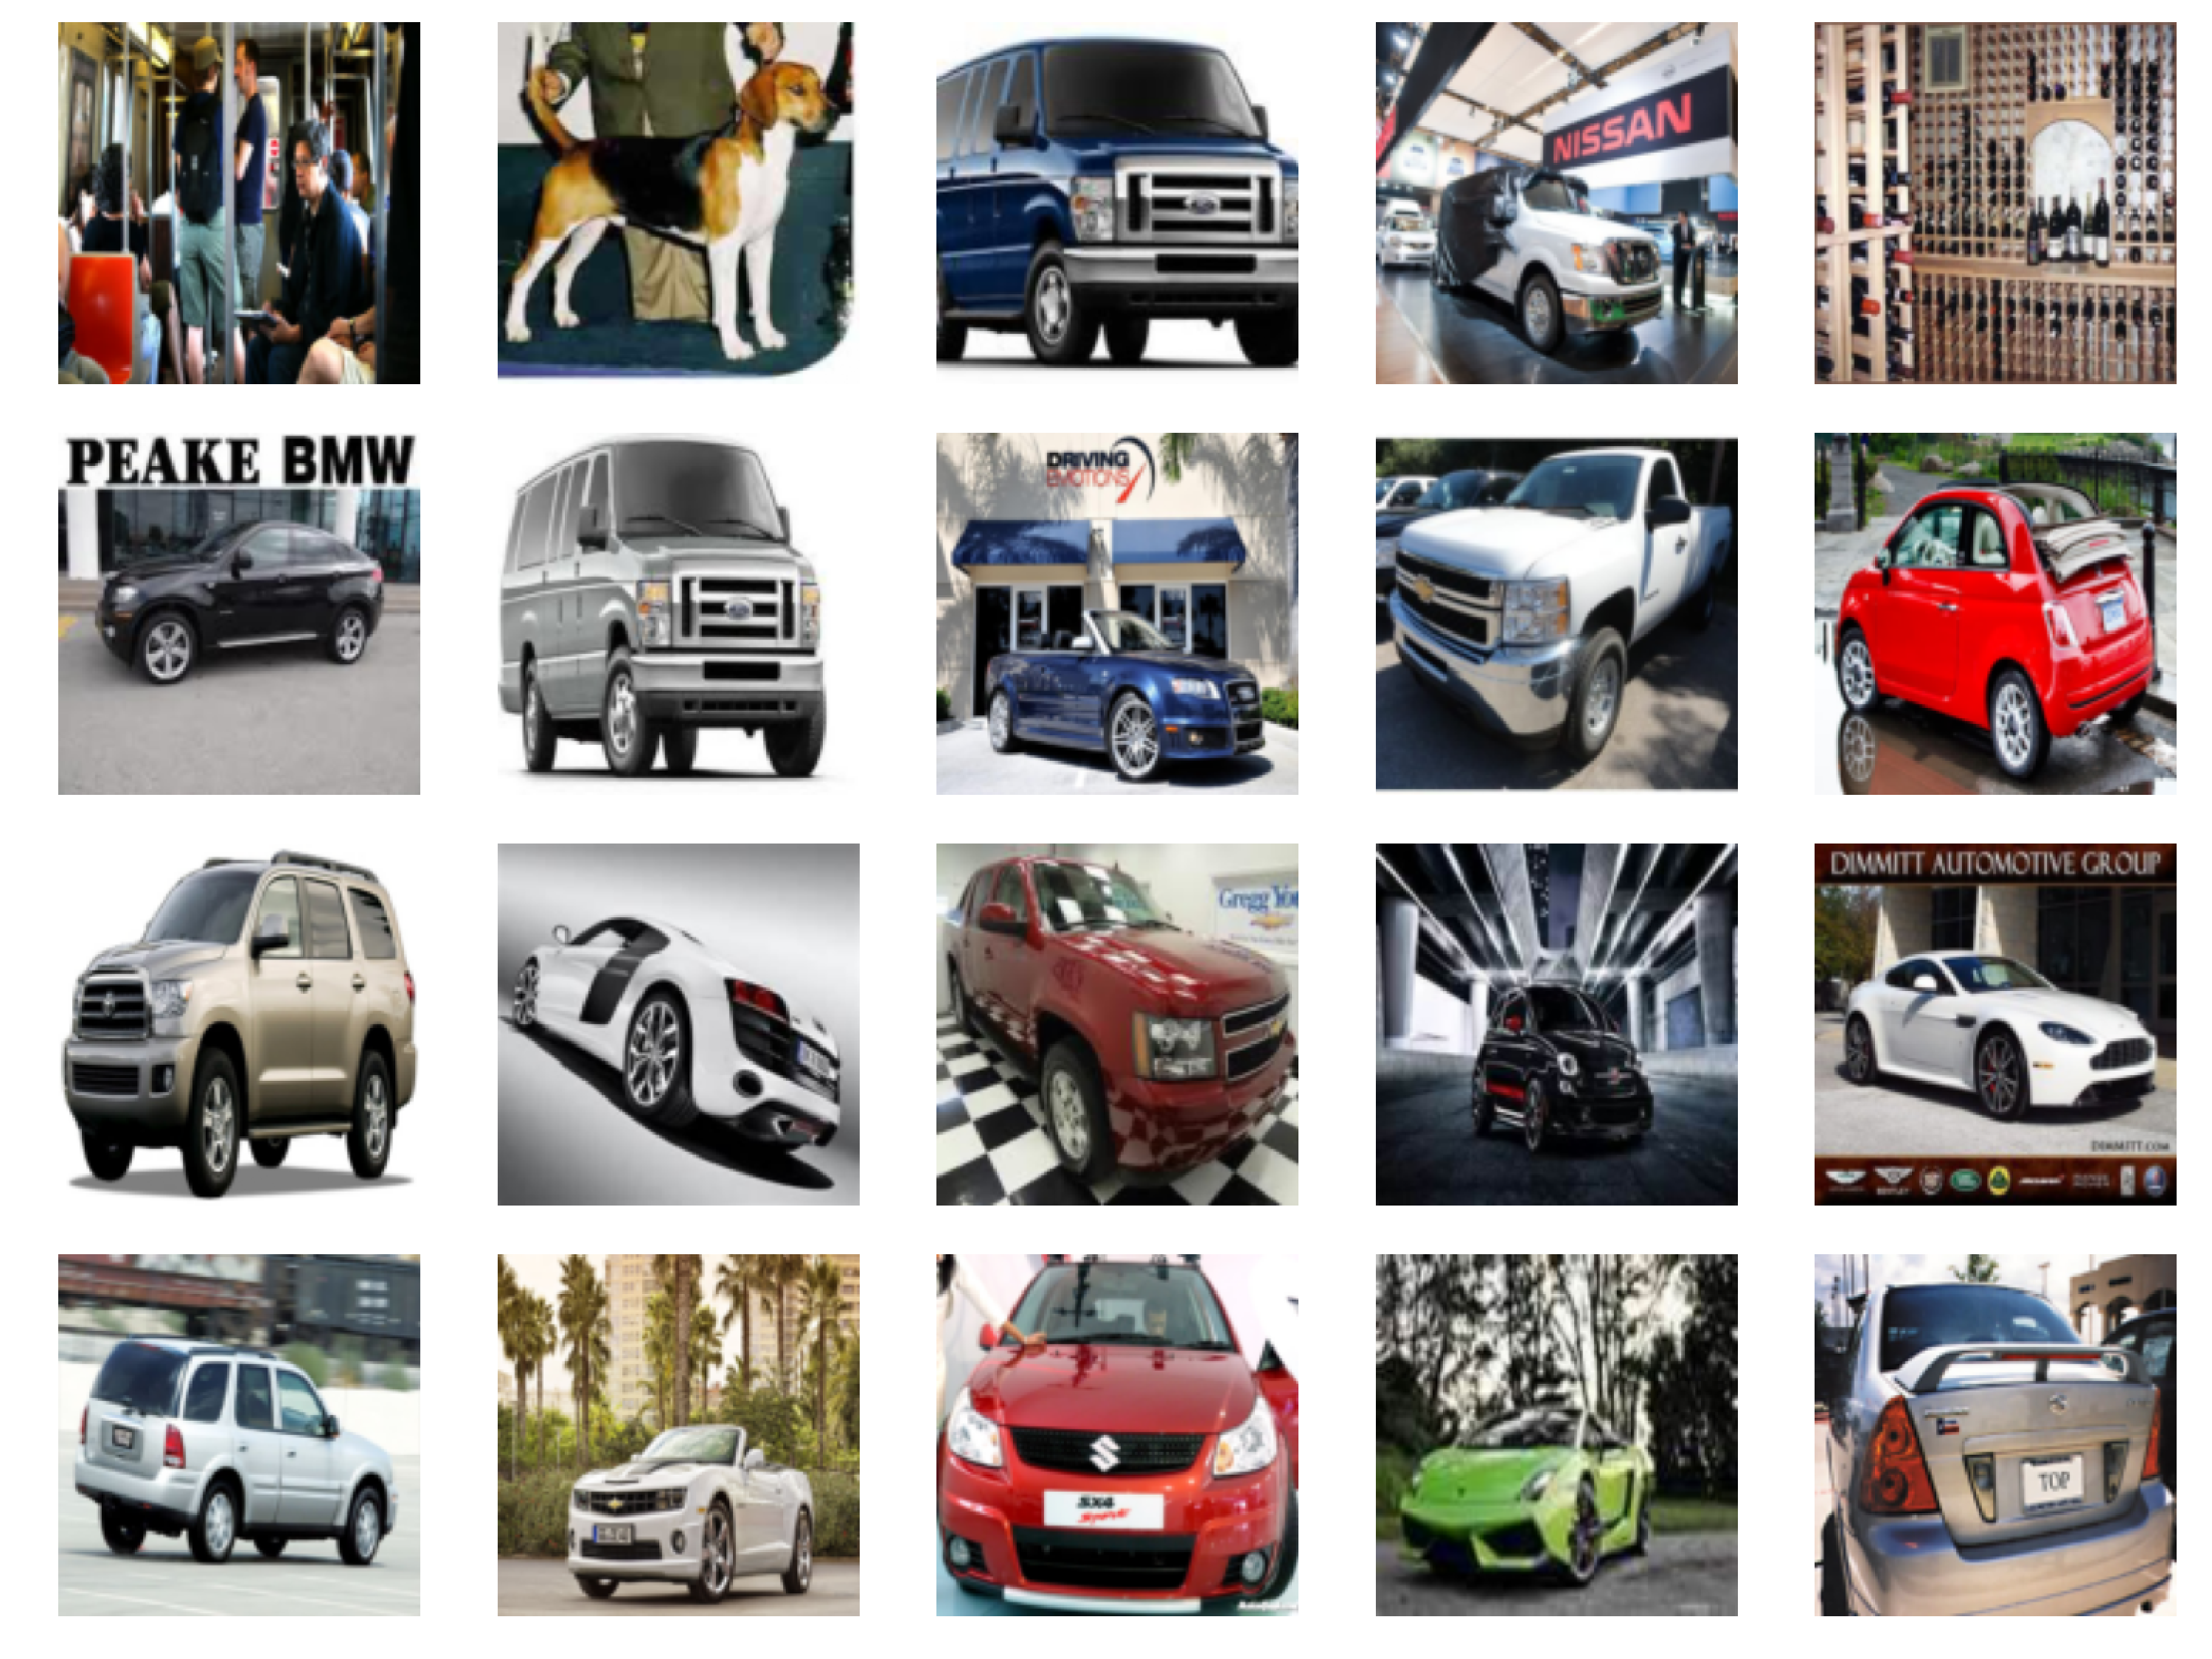
\includegraphics[width=12cm]{images/biggest_errors}
		\caption{Exemples d'images mal reconstruites}
		\label{fig:acp_reconstructionsb}
	\end{subfigure}
	\caption{Exemples d'images qui sont bien reconstruites (a) et mal reconstruites (b) selon la méthode ACP appliquée sur le jeu de données d'entraînement de \textit{ImageNet}.}
	\label{fig:acp_reconstructions}
\end{figure}

En analysant la figure \ref{fig:acp_reconstructions}, on remarque que les images bien reconstruites sont des images relativement "simples". Les images de la classe "normale" à la figure \ref{fig:acp_reconstructionsa} montrent des voitures avec une vue relativement éloignée. Les arrières plans sont également plutôt simple, avec des couleurs assez unies. À l'inverse, les images les moins biens reconstruites (figure \ref{fig:acp_reconstructionsb}) sont plus "complexes". Par exemple, on voit les voitures de très près, avec beaucoup de détails. Aussi, les arrières plans sont beaucoup plus complexes, avec différentes couleurs et formes. Au final, on pourrait conclure que la méthode basée sur l'ACP discrimine sur la complexité de l'image plutôt que sur le contenu (voitures versus autres). La méthode AE performe un peu mieux que l'ACP, mais elle obtient tout de même des aires sous la courbe ROC inférieures à 0.6, et ce, pour les 3 scénarios de contamination. On pourrait penser que l'autoencodeur, avec la perte orientée sur le contenu \textit{perceptual loss}, gère un peu mieux ces différents éléments (vues, couleurs, arrière-plan, etc), mais cela n'est pas suffisant pour obtenir des performances optimales. Au final, les méthodes basées sur l'erreur de reconstruction nous apparaissent moins pertinentes lorsque nous devons faire la détection d'anomalies dans des images de complexités et de styles différents.
 

\subsubsection{Analyse des représentations latentes} \label{analyse_lat_cars}

Dans la section \ref{cadre_decisionnel}, nous avons mentionné qu'il fallait analyser les statistiques de distance afin de savoir si une statistique de distance élevée est signe d'anomalie ou de normalité. Pour ce faire, il suffit de visualiser un échantillon d'images de notre jeu de données d'entraînement ayant des statistiques de distance élevées et un autre échantillon d'images ayant des statistiques de distance faibles. Dans la figure \ref{fig:latentes_images}, on peut voir quelques exemples provenant de ces échantillons. On remarque assez rapidement que les observations ayant des statistiques de distance faibles proviennent de notre classe "anormale". À l'inverse, les observations ayant des statistiques de distance élevées proviennent de notre classe "normale", soit des images de voitures. On remarque que les voitures de la figure \ref{fig:latentes_images} sont presque toutes des voitures rouges. Il est possible que les représentations latentes ce type de voitures soient situées dans un espace similaire et le plus éloigné de la $N(0,1)$. Nous avons voulu valider si la couleur de la voiture avait un impact significatif dans la prise de décision. Pour ce faire, nous avons pré-sélectionné un échantillon d'images de voitures de différentes couleurs et avons calculé le score d'anomalie pour ces images. À la figure \ref{fig:random_samples}, on peut voir que les voitures rouges obtiennent des scores d'anomalie plutôt élevés, même une avec un score sous la valeur du seuil de filtration $\alpha$. Cela nous permet de confirmer que ce n'est pas la couleur de la voiture seulement qui a un impact.

\begin{figure}[htb]
	\centering
	\begin{subfigure}{6cm}
		\centering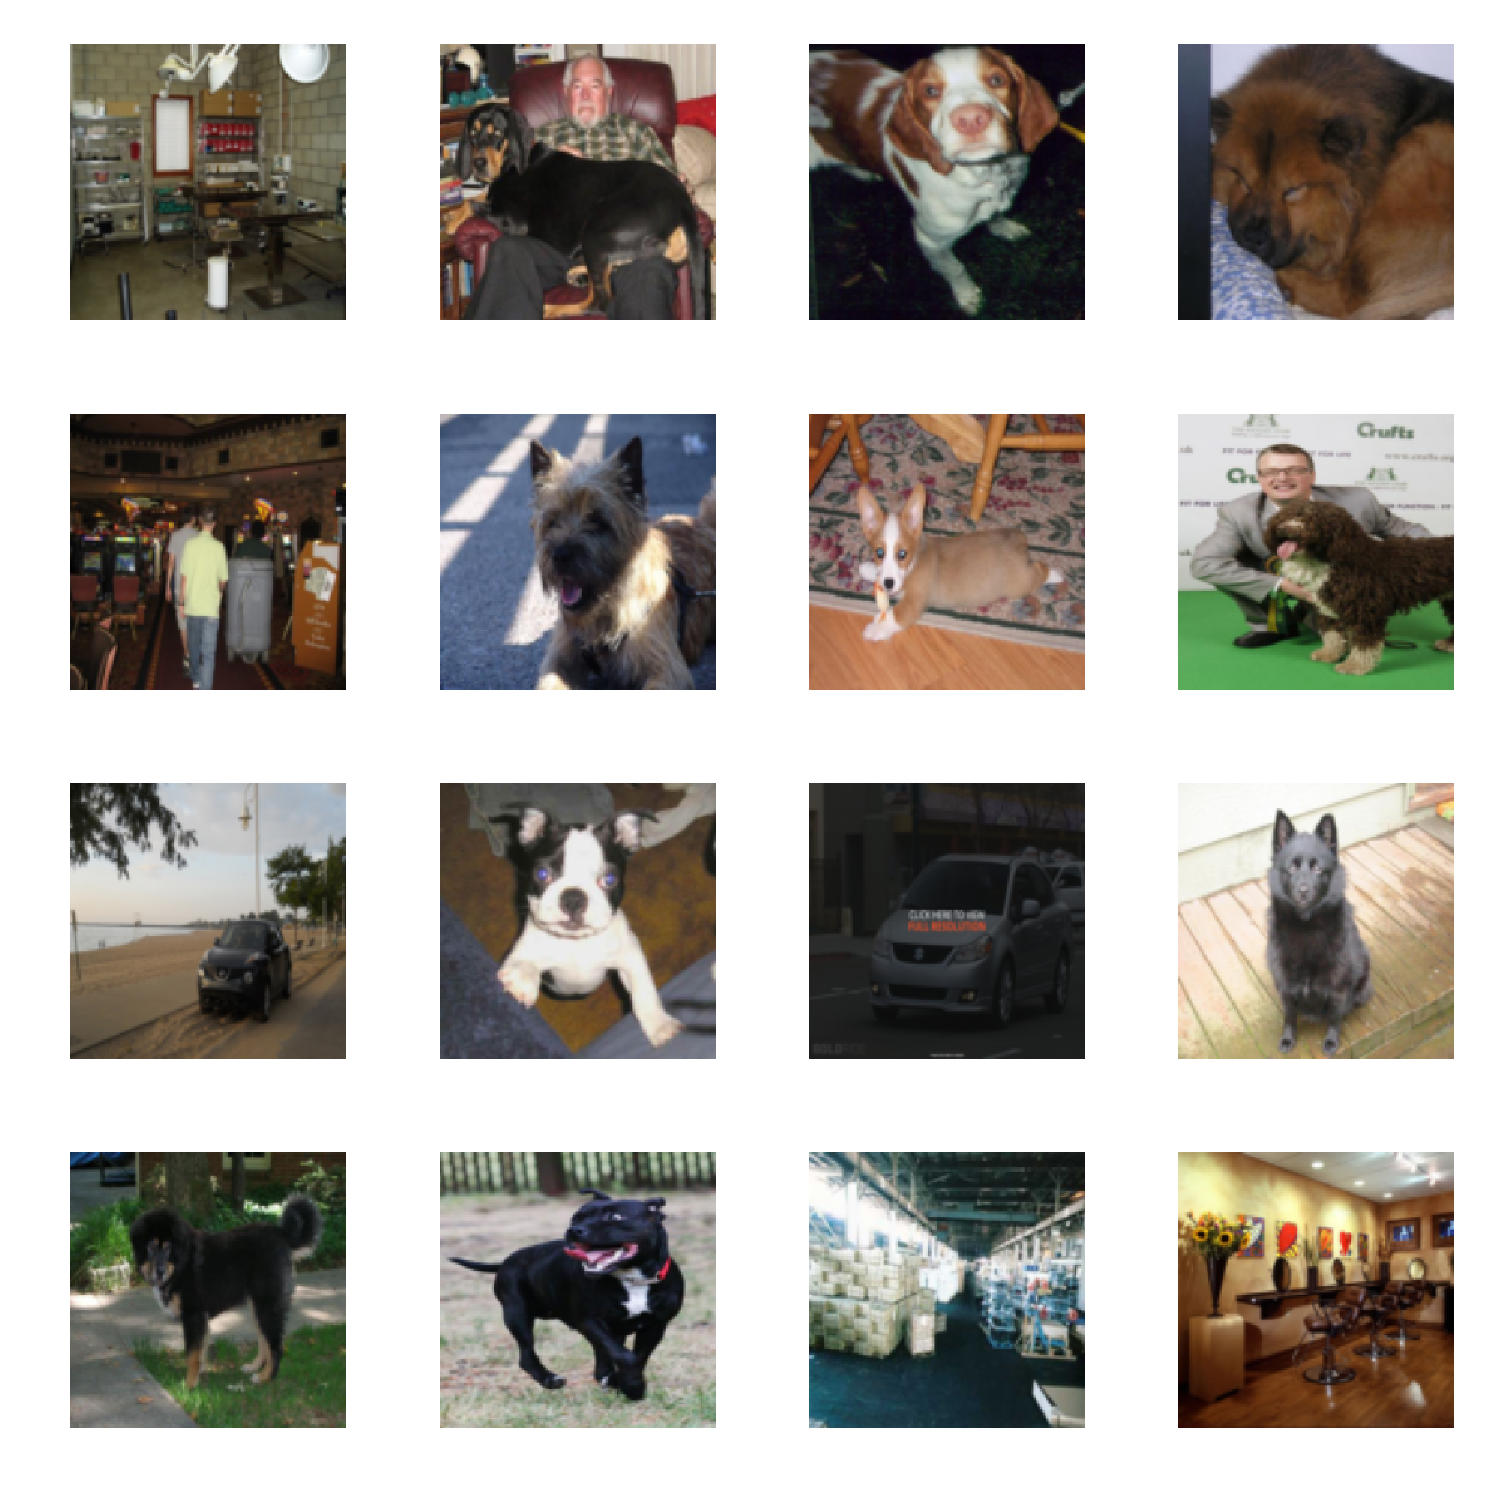
\includegraphics[width=6cm]{images/images_davae/cars_small_distance}
		\caption{Statistiques de distance faible}
	\end{subfigure}
	\begin{subfigure}{6cm}
		\centering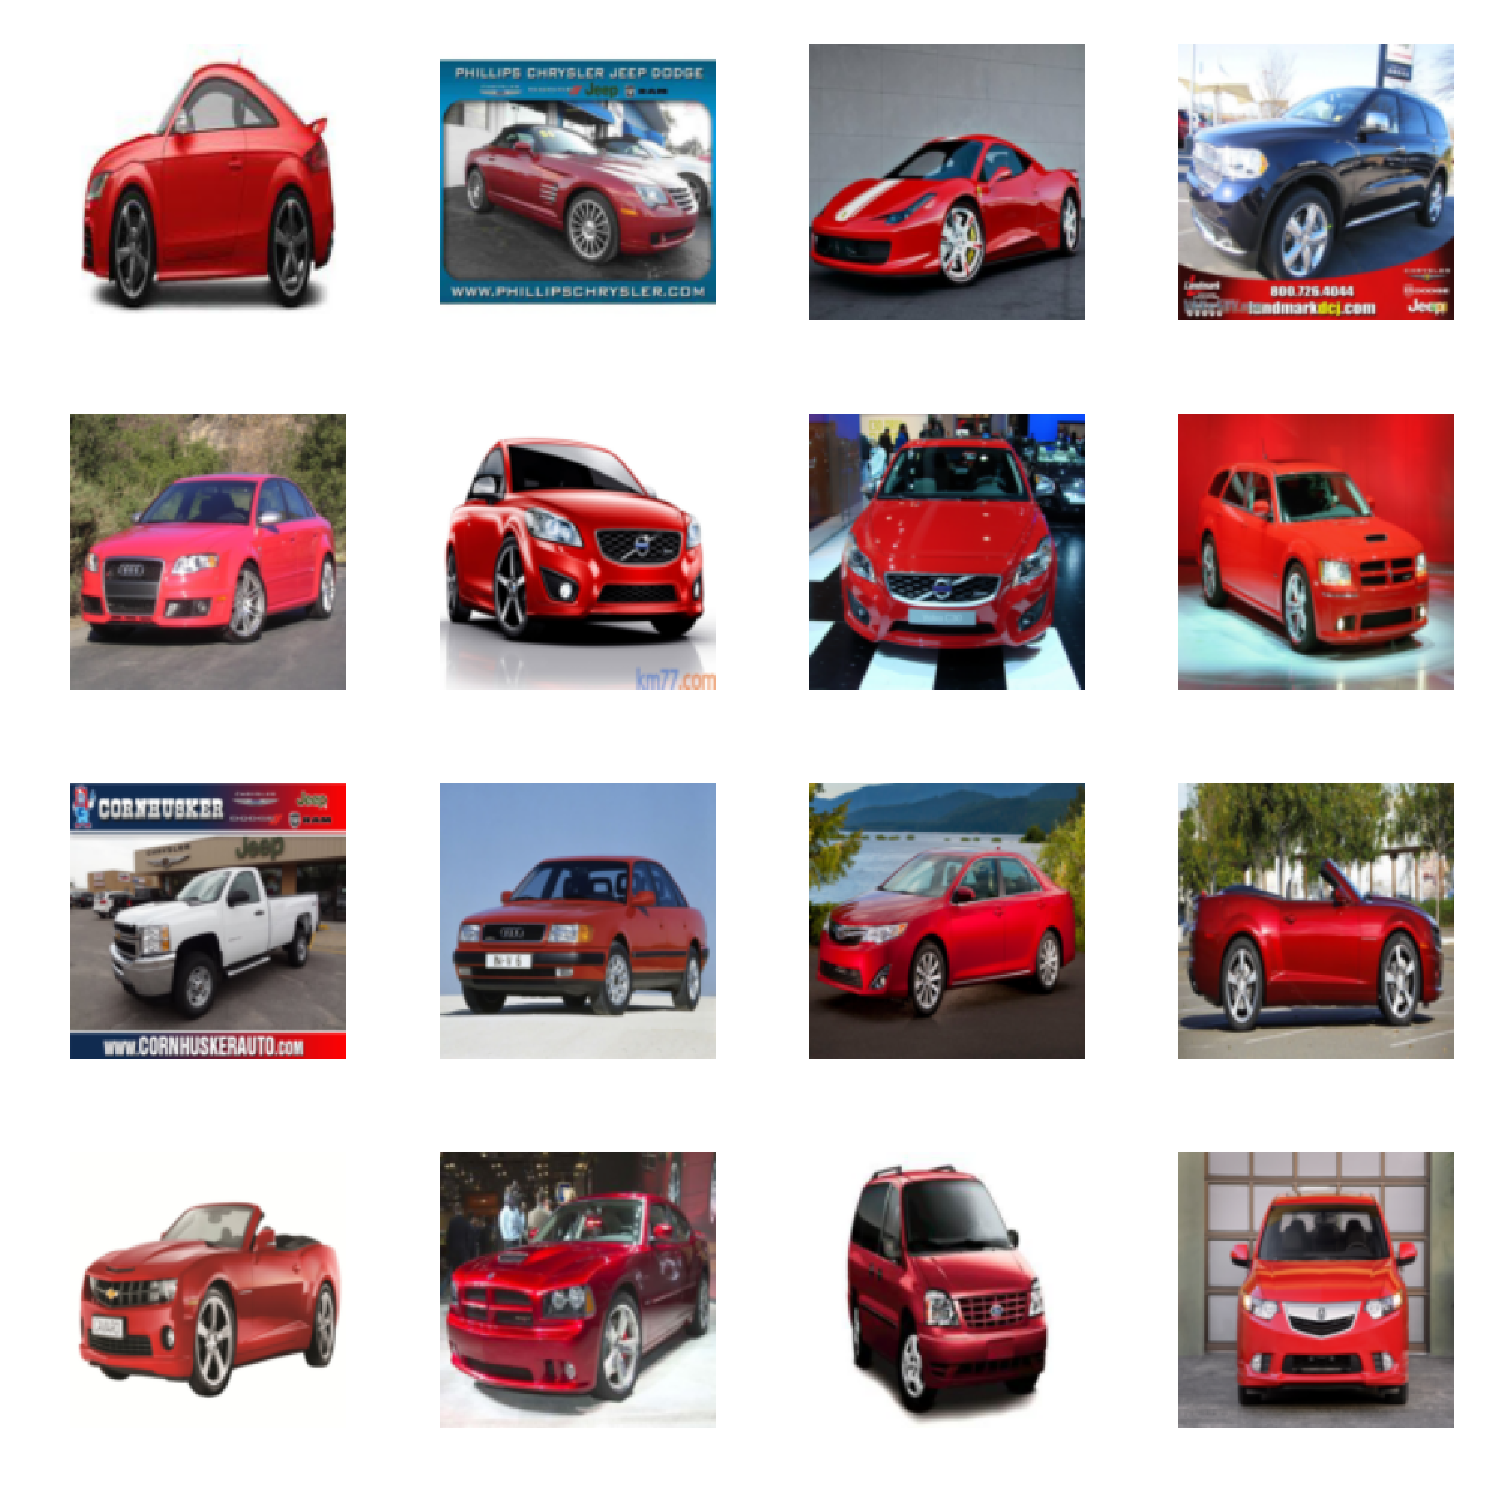
\includegraphics[width=6cm]{images/images_davae/cars_large_distance}
		\caption{Statistiques de distance élevées}
	\end{subfigure}
	\caption{Échantillons d'images provenant du jeu de données d'entraînement ayant des statistiques de distance faibles (a) et élevées (b) pour le scénario "Plus" du jeu de données \textit{ImageNet}.}
	\label{fig:latentes_images}
\end{figure}

\begin{figure}[htb]
	\centering
	\centering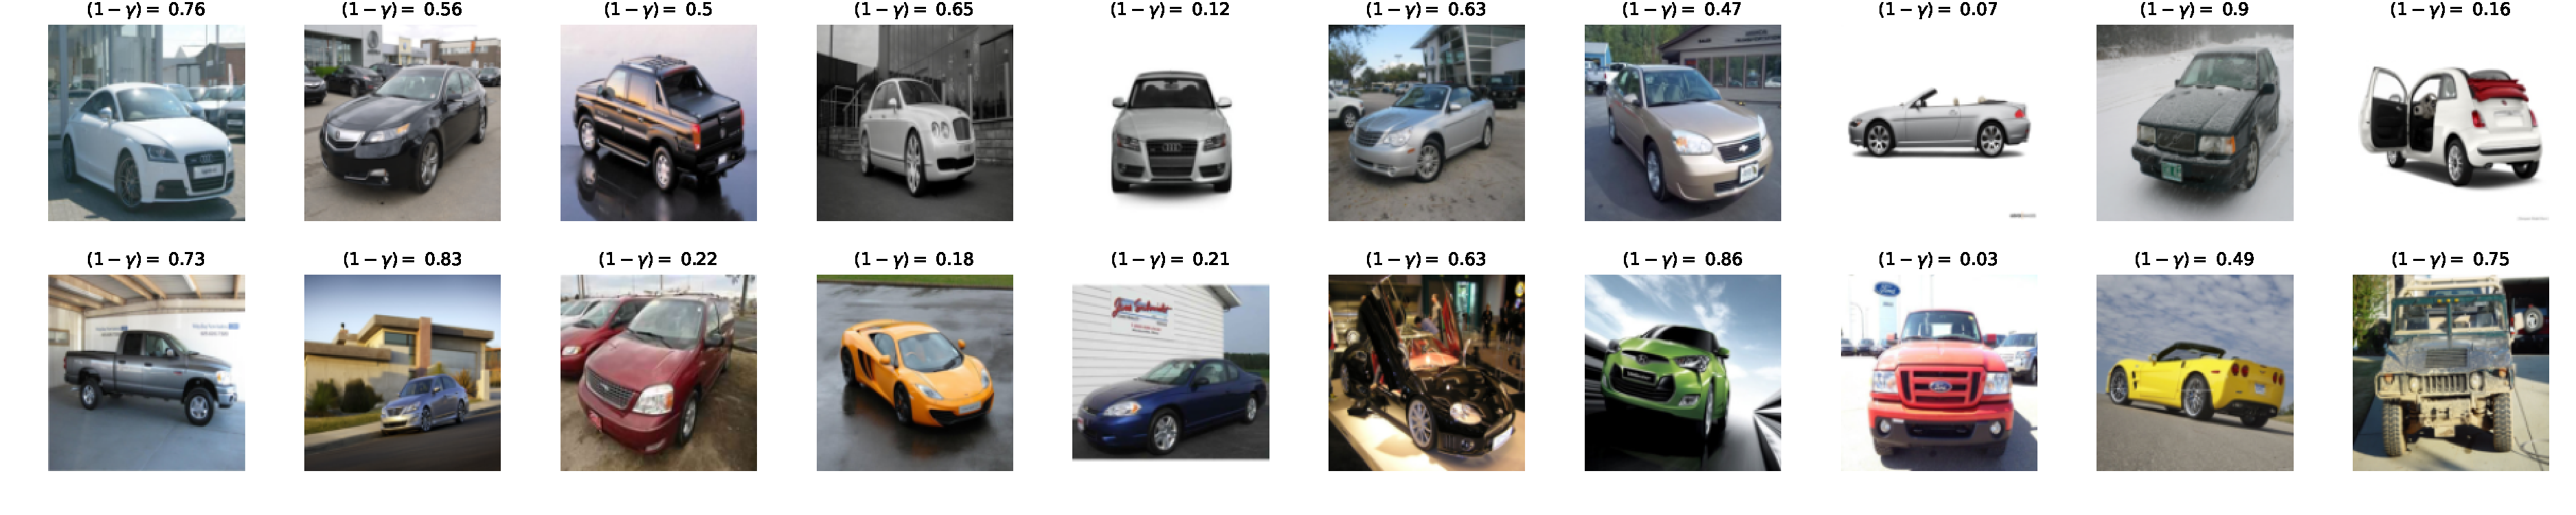
\includegraphics[width=\linewidth]{images/random_examples}
	\caption{Échantillons d'images pré-sélectionnées avec l'inverse de leur score d'anomalie ($1-\gamma$). Le score a été calculé selon le modèle DA-VAE du scénario "Plus" sur le jeu de données \textit{ImageNet}.}
	\label{fig:random_samples}
\end{figure}

De cette manière, il est possible de conclure que nous nous retrouvons dans le scénario où les représentations latentes des observations "normales" sont plus éloignées de la $N(0,I)$ (voir les deux scénarios décrits à \ref{liste_scenarios}). À la figure \ref{fig:cars_latent_stats}, on peut confirmer cette observation alors qu'on voit que les valeurs moyennes des $\boldsymbol{\mu}$ et $\boldsymbol{\sigma}$ des observations "normales" sont plus éloignées de la $N(0,I)$. Dans cette figure, on calcule pour chaque observation du jeu de données d'entraînement, la valeur moyenne sur les 25 dimensions latentes des vecteurs $\boldsymbol{\mu}$ et $\boldsymbol{\sigma}$. La différence est beaucoup plus évidente pour le vecteur latent $\boldsymbol{\sigma}$ que pour $\boldsymbol{\mu}$. Pour $\boldsymbol{\mu}$, les observations "normales" sont légèrement plus centrées à 0, mais les observations "anormales" s'éloignent moins de la valeur centrée de 0. À la figure \ref{fig:pca_cars}, nous avons réalisé une analyse en composantes principales sur les vecteurs $\boldsymbol{\mu}$ et $\boldsymbol{\sigma}$ et avons conservé les 2 premières composantes principales. Cela nous permet d'obtenir une visualisation en 2 dimensions des représentations latentes des observations "normales" et des anomalies. On peut voir que les 2 groupes sont relativement bien séparés sur les 2 premières composantes principales. On peut également voir la projection en 2 dimensions du point $(\boldsymbol{0_{m}}, \boldsymbol{1_{m}})$, soit le carré noir. On remarque que les anomalies (points bleus) semblent légèrement plus près du carré noir que les observations "normales". Il faut rappeler que la projection en 2 dimensions conserve approximativement 50\% de la variabilité totale des représentations latentes.

\begin{figure}[H]
	\centering
	\begin{subfigure}{12cm}
		\centering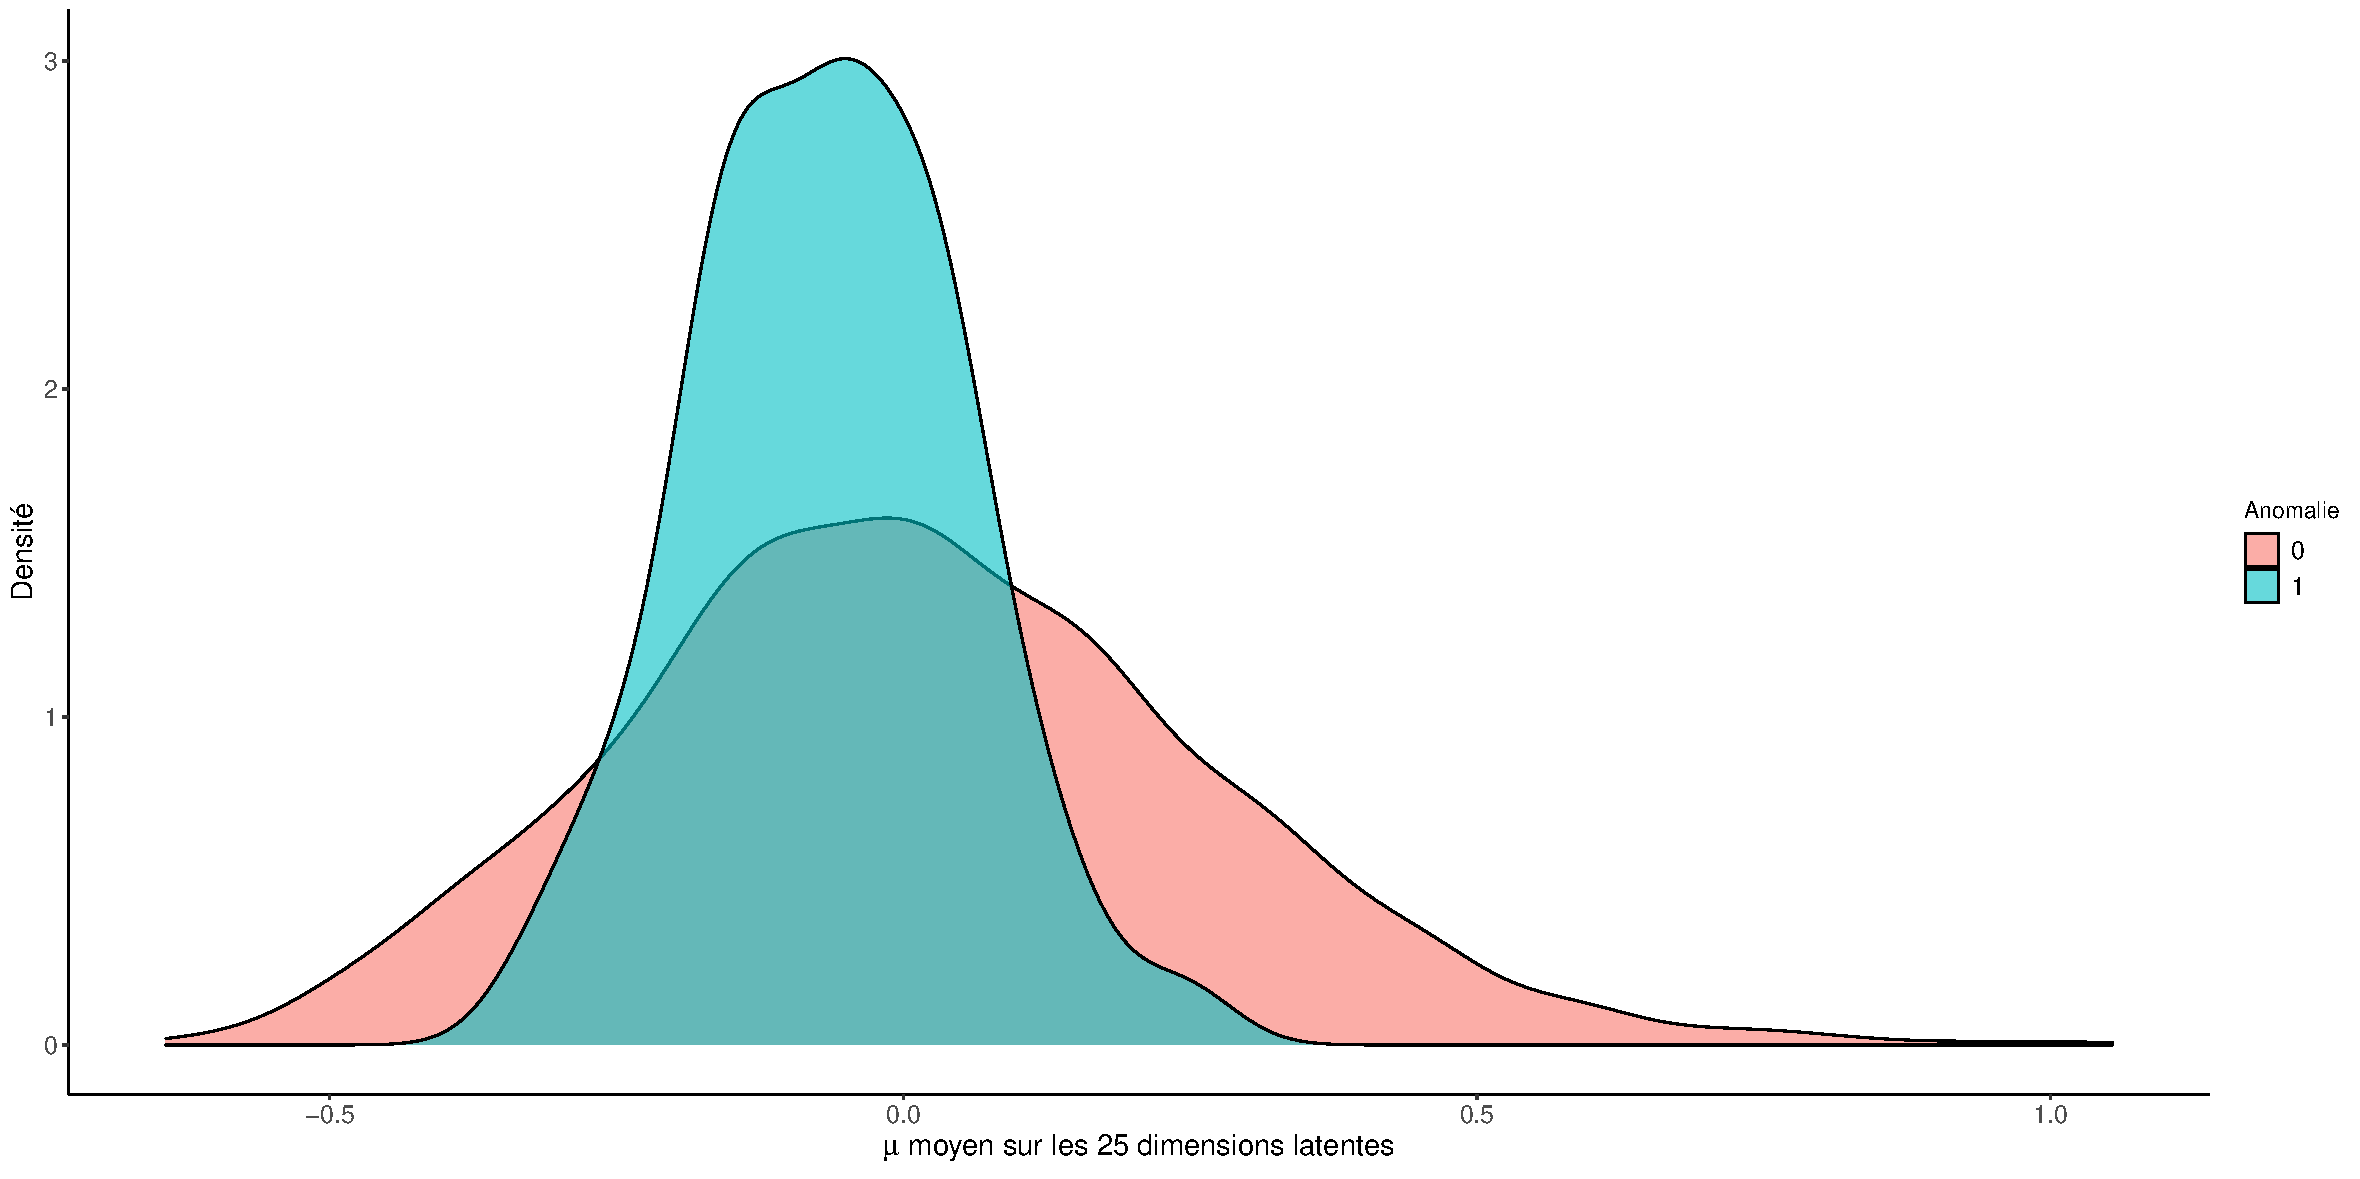
\includegraphics[width=12cm, height=6cm]{images/latent_stats/plot_mu}
		\caption{Distribution des $\boldsymbol{\mu}$ moyens}
	\end{subfigure}
	\begin{subfigure}{12cm}
		\centering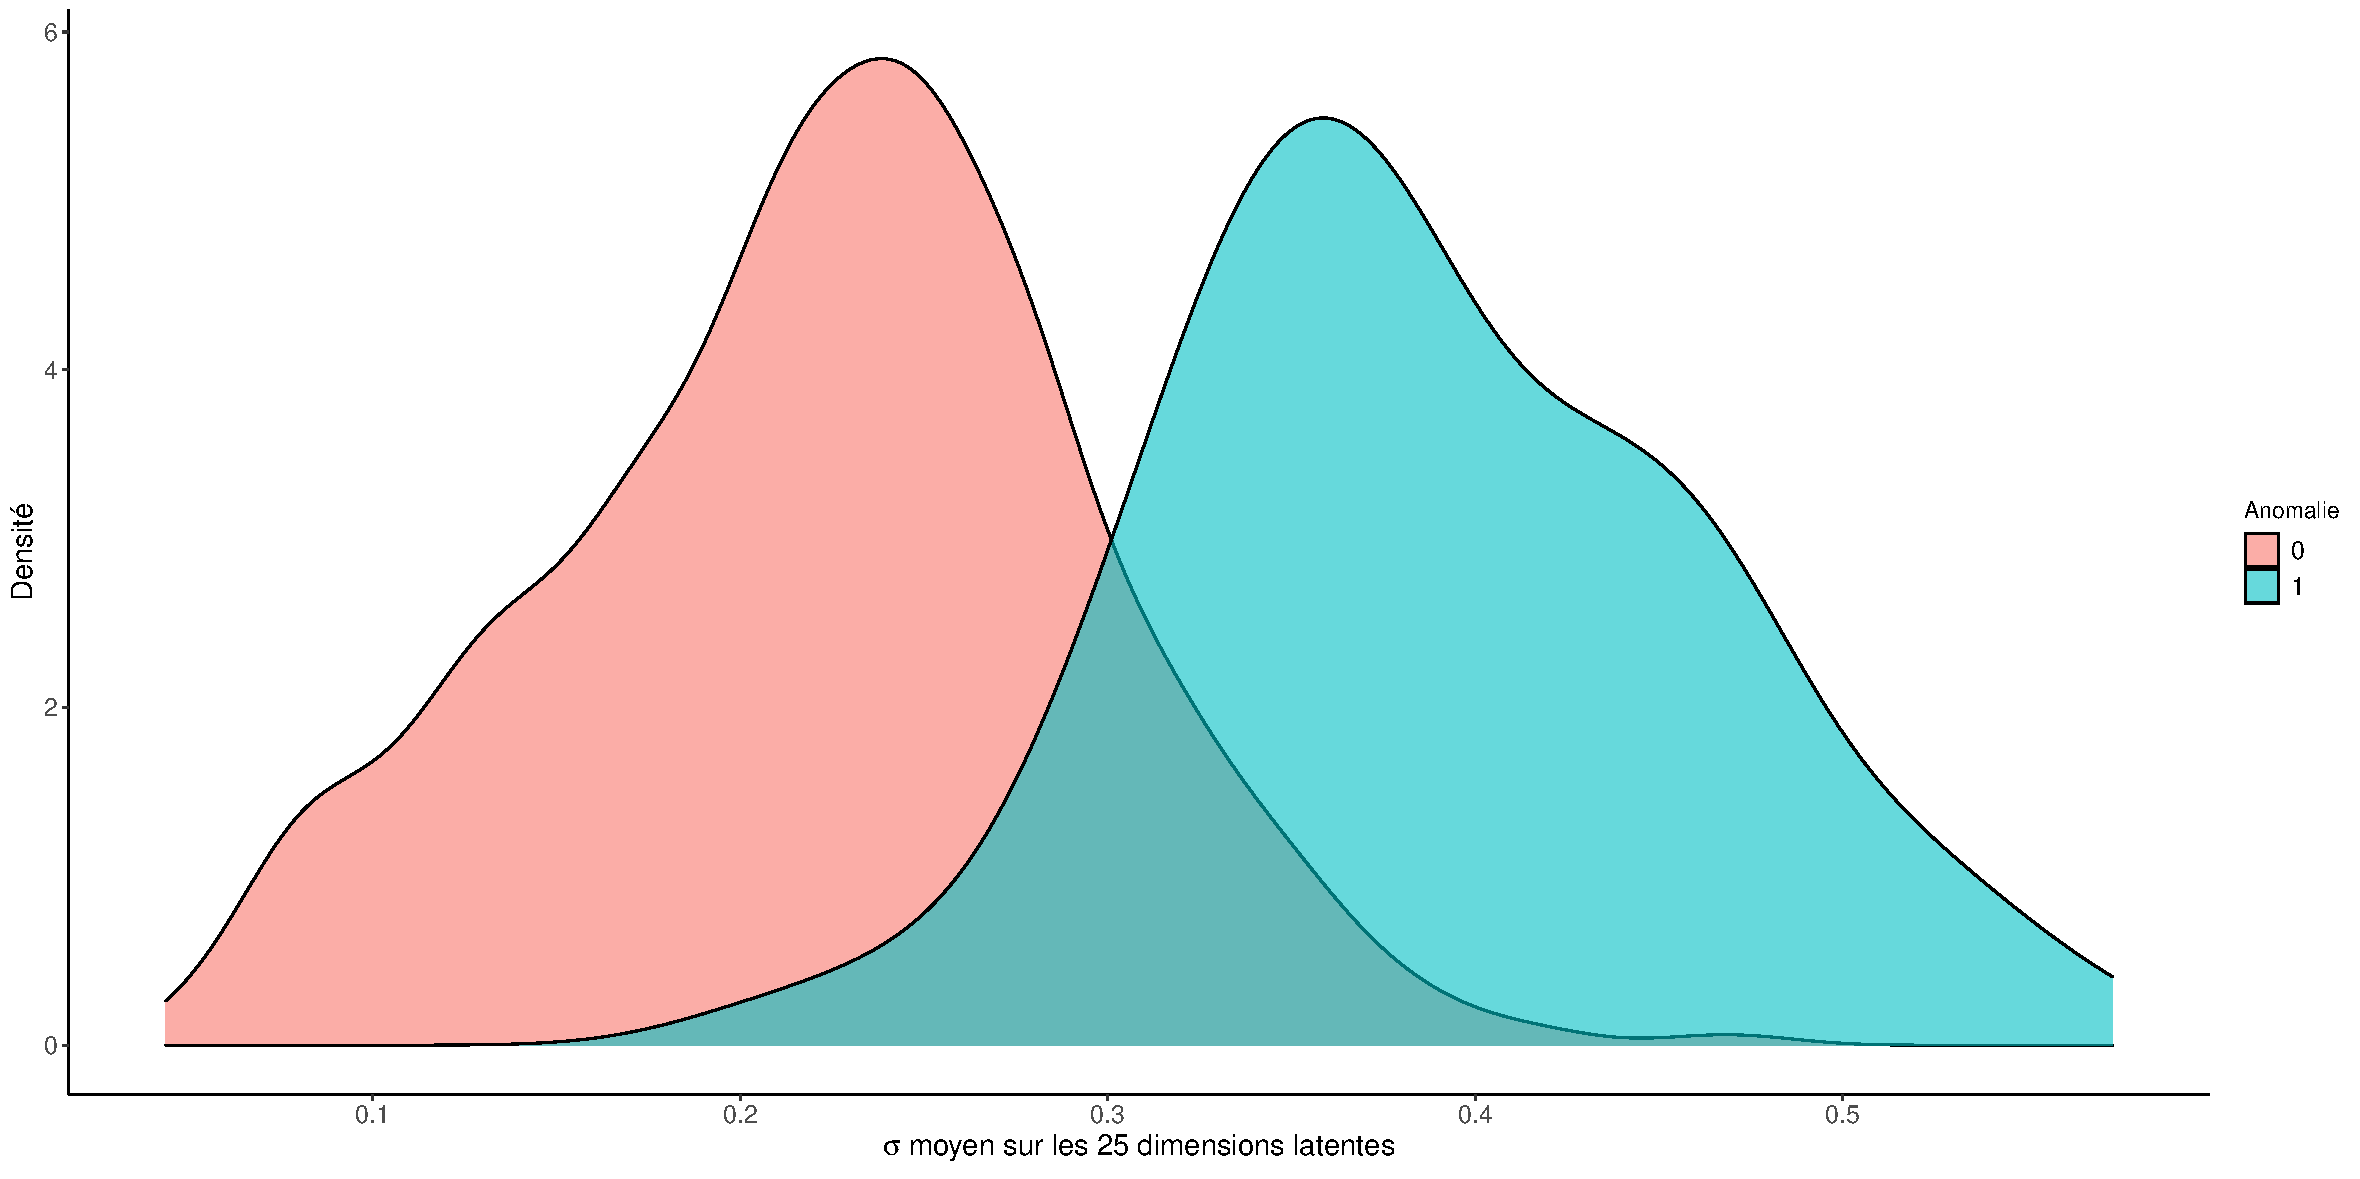
\includegraphics[width=12cm, height=6cm]{images/latent_stats/plot_sigma}
		\caption{Distribution des $\boldsymbol{\sigma}$ moyens}
	\end{subfigure}
	\caption{Moyenne des $\boldsymbol{\mu}$ et $\boldsymbol{\sigma}$ des représentations latentes du jeu de données d'entraînement sur le jeu de données \textit{ImageNet}.}
	\label{fig:cars_latent_stats}
\end{figure}

\begin{figure}[htb]
	\centering
	\centering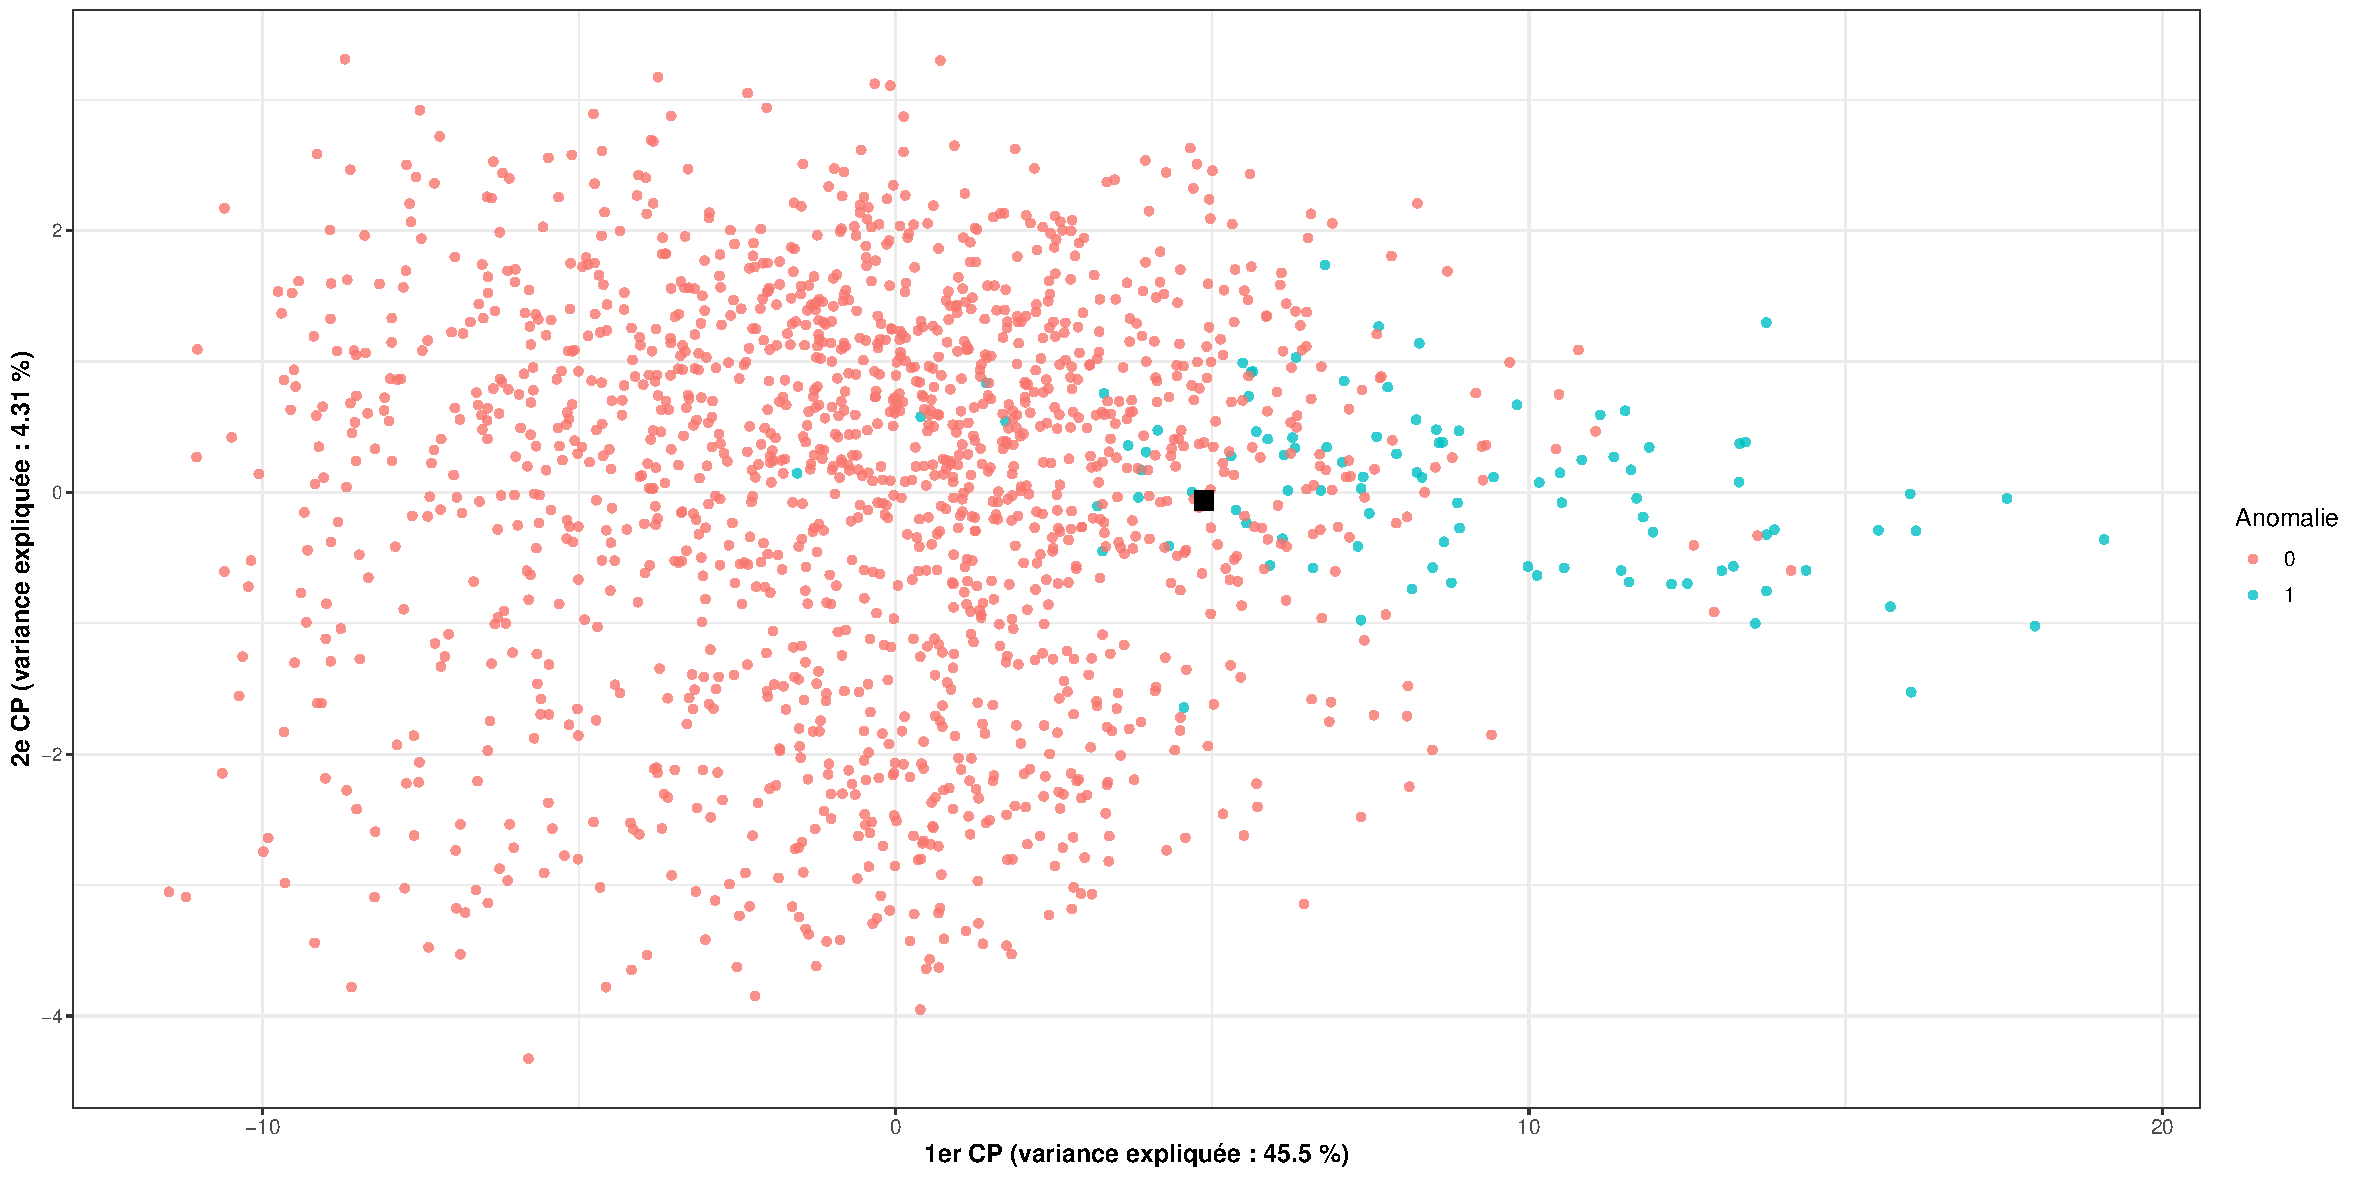
\includegraphics[width=\linewidth]{images/plot_pca_cars}
	\caption{Graphique des 2 premières composantes principales réalisé sur les vecteurs $\boldsymbol{\mu}$ et $\boldsymbol{\sigma}$ du jeu de données d'entraînement de \textit{ImageNet} appliqué sur le scénario de contamination "Plus".}
	\label{fig:pca_cars}
\end{figure}


\subsubsection{Analyse de la perte en entraînement}

Dans la section \ref{beta_schedule}, nous avons présenté l'horaire de l'hyperparamètre $\beta$ utilisé selon l'itération d'entraînement de l'autoencodeur variationnel. Cet hyperparamètre, utilisé dans les méthodes ISOF-VAE et DA-VAE, donne plus ou moins d'importance à la composante de perte associée au critère de Kullback-Leibler. Notre objectif était de mettre l'accent sur la composante de reconstruction $(\beta = 0)$ dans les premières itérations pour ensuite augmenter la régularisation en augmentant l'hyperparamètre $\beta$ pendant quelques itérations. La figure \ref{fig:cars_kld_perc} illustre la composition de notre perte totale au fil des itérations d'entraînement. La figure illustre le pourcentage de la perte provenant du critère de Kullback-Leibler. L'autre composante de la perte est associée à la reconstruction. On peut voir que les 5 premières itérations sont composées uniquement de la composante de reconstruction. Cela est dû à notre hyperperamètre $\beta=0$. Par la suite, la composante de Kullback-Leibler prend plus d'importance et tend finalement vers une valeur près de 0 dans les dernières itérations. Il est rassurant de voir que l'horaire que nous avons établi pour l'hyperparamètre $\beta$ est cohérent avec la composition de la perte obtenue.

\begin{figure}[H]
	\centering
	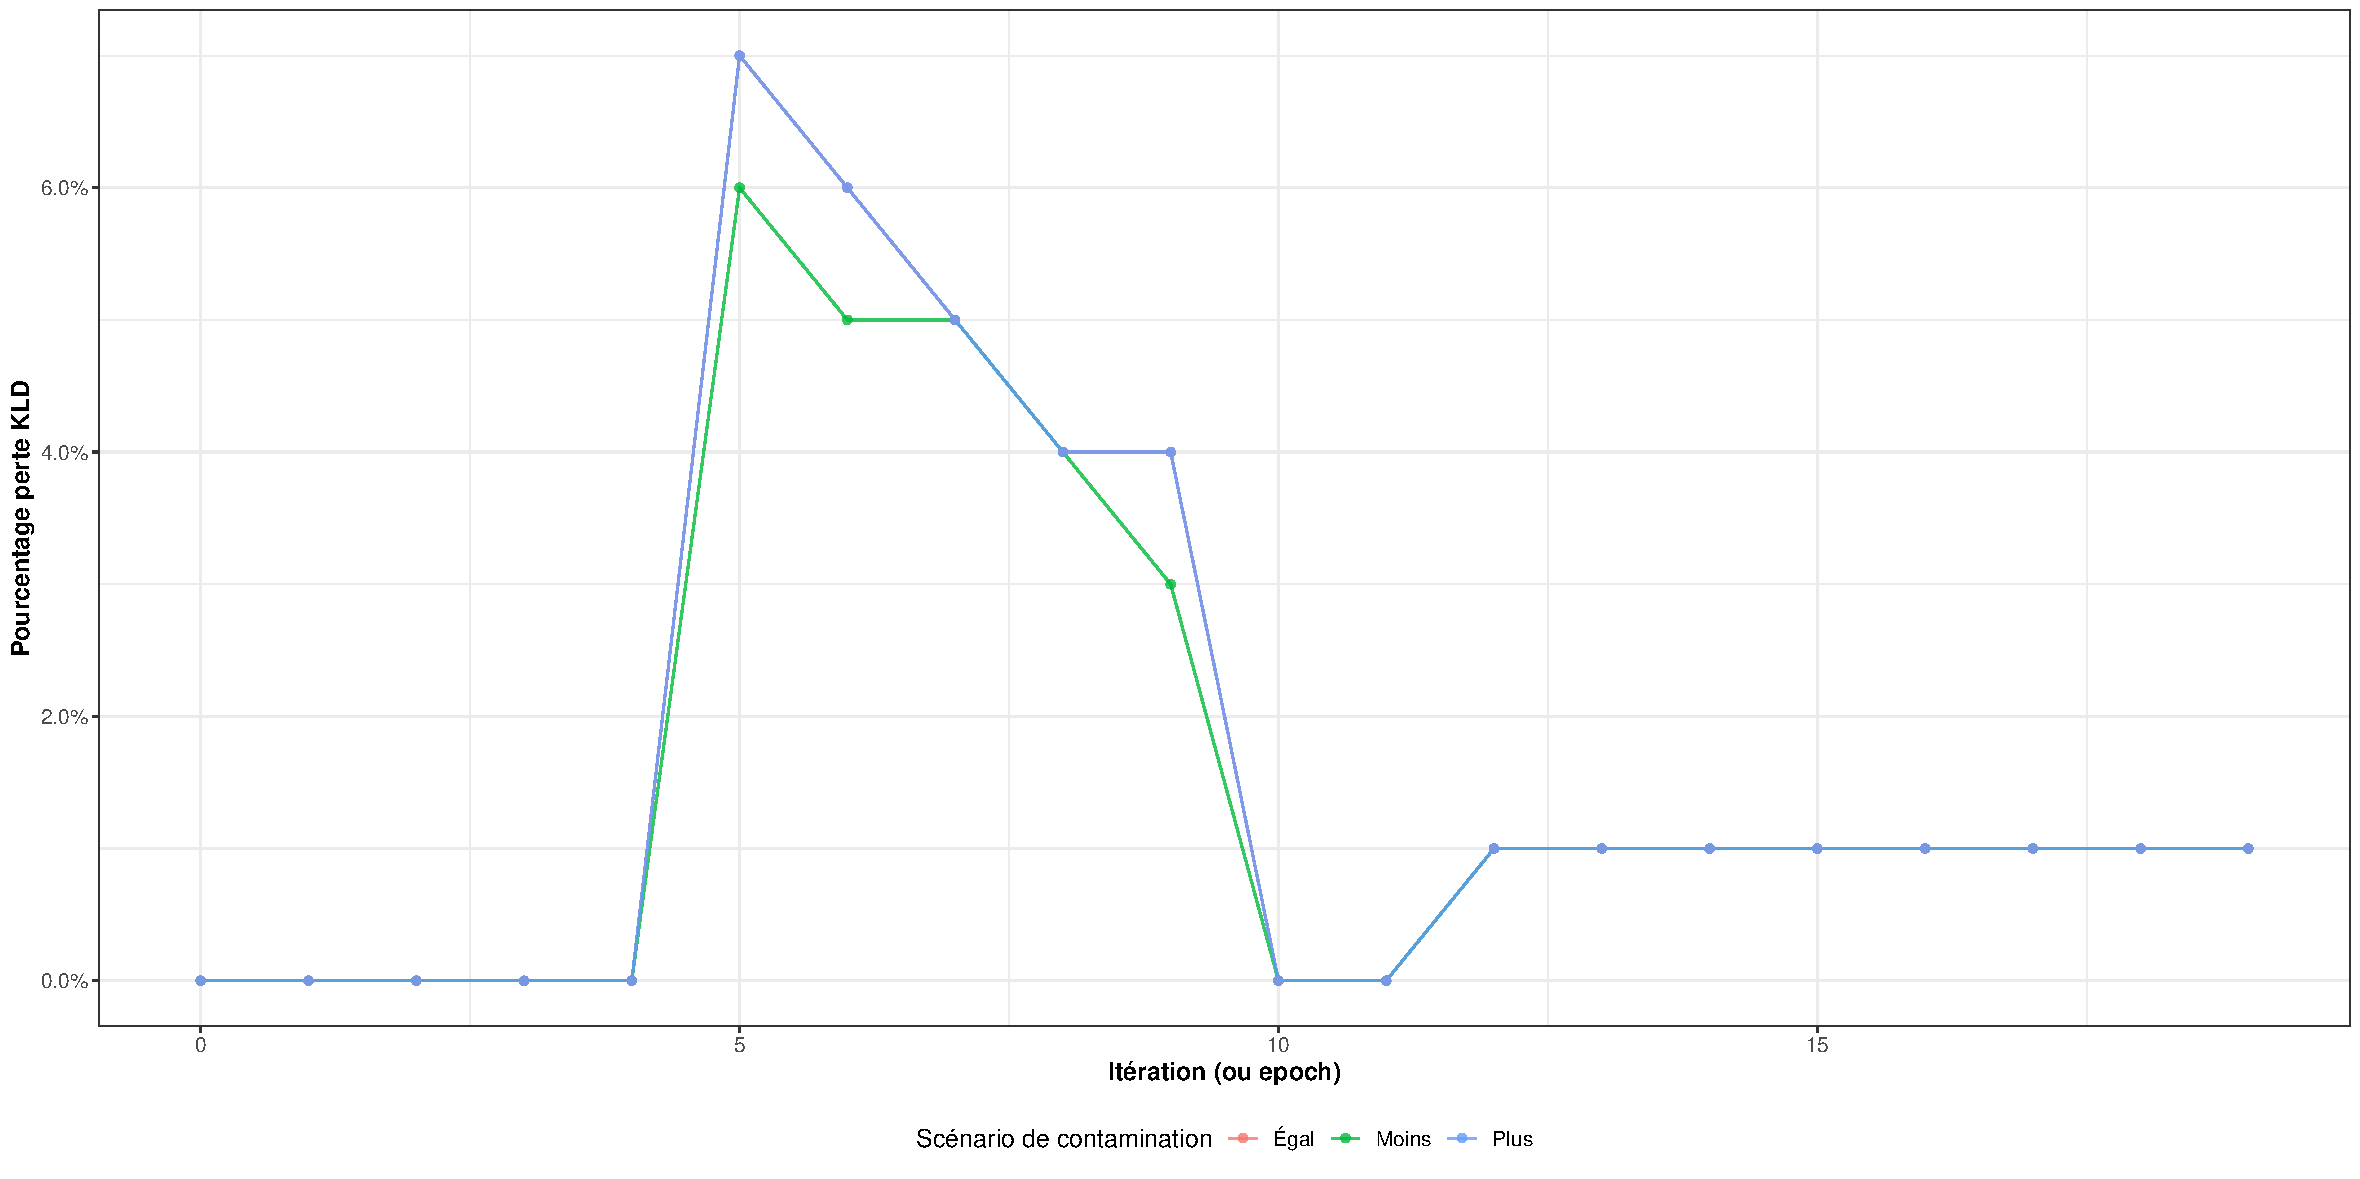
\includegraphics[width=\linewidth]{images/kld_cars.pdf}
	\caption{Pourcentage du critère de Kullback-Leibler dans la perte totale selon l'itération d'entraînement et le scénario de contamination. Ces résultats sont tirés du scénario de contamination "Plus" pour le jeu de données \textit{ImageNet}.}
	\label{fig:cars_kld_perc}
\end{figure}


\subsubsection{Génération d'images}

Comme mentionné dans la section \ref{background-vae}, les autoencodeurs variationnels ont la particularité d'avoir une représentation latente continue. En effet, cela est dû au fait que le vecteur latent $\boldsymbol{z}$ est obtenu en combinant une simulation d'une loi $N(0,I)$ avec les vecteurs $\boldsymbol{\mu}$ et $\boldsymbol{\sigma}$ appris par le modèle (voir équation \ref{eq:latent_formula}). Étant donné la composante de perte de Kullback-Leibler appliquée dans l'optimisation des paramètres, ces 2 vecteurs devraient s'approcher des vecteurs $(\boldsymbol{0_{m}}, \boldsymbol{1_{m}})$ où $m$ correspond à la longueur de la représentation latente. Après l'entraînement de l'autoencodeur, il est possible de valider le comportement du décodeur par rapport à une simulation $N(0,I)$. La figure \ref{fig:generated_cars} montre des exemples d'images générées à partir de simulations de loi $N(0,I)$ et reconstruites par la partie décodeur du DA-VAE. Ces images, générées de toute pièce, illustrent bien qu'une représentation latente provenant d'une loi $N(0,I)$ donne un résultat qui s'apparente à une voiture ou aux caractéristiques fréquentes d'une voiture (roues, phares, pare-brise).

\begin{figure}[htb]
	\centering
	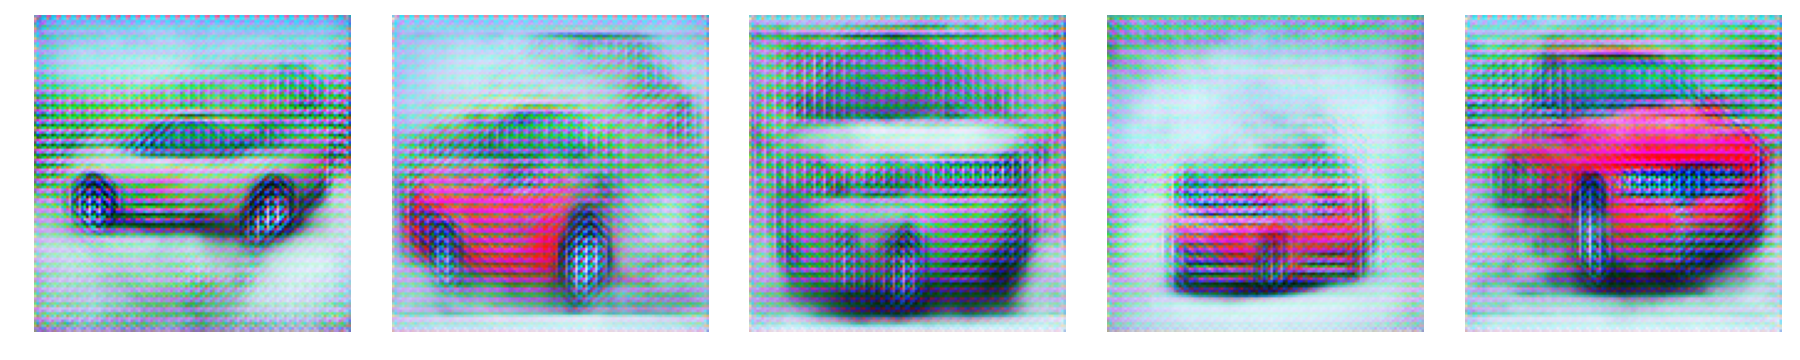
\includegraphics[width=\textwidth]{images/generated_cars}
	\caption{Exemples d'images générées par le modèle DA-VAE en utilisant seulement la partie décodeur de l'autoencodeur ainsi que des simulations provenant d'une loi $N(0,I)$.}
	\label{fig:generated_cars}
\end{figure}

\subsection{Résultats sur \textit{MNIST}}

Dans le tableau \ref{tab:auc_mnist}, on peut voir les performances en aire sous la courbe ROC pour les différents scénarios de test réalisés sur \textit{MNIST}. Premièrement, on remarque que toutes les approches donnent des résultats performants avec des aires sous la courbe généralement supérieures à 0.85, et même parfois très près de 1. Cette observation vient témoigner du fait qu'étant donné la nature plus simple des données, il est probablement plus facile de faire la détection d'anomalies. En regardant de plus près les résultats des 4 approches, on remarque que notre approche DA-VAE est rarement meilleure que les méthode AE ou ACP en aire sous la courbe ROC moyenne. La variabilité autour de la métrique est aussi légèrement plus élevée pour l'approche DA-VAE. Par contre, les résultats sont généralement près des meilleures approches. De plus, l'intervalle avec 2 écart-types autour de la moyenne nous permet de conclure que les autres méthodes ne sont pas significativement meilleures que DA-VAE. Notre approche montre également les meilleurs résultats en aire sous la courbe ROC pour le scénario de test 6, et ce, pour les 3 scénarios de contamination différents. Le scénario de test 6 est celui qui considère le chiffre "6" comme "normal" et tous les autres comme la classe "anormale". Étant donné la nature plus simple des images, les méthodes basées sur la reconstruction (ACP et AE) semblent être celles qui fonctionnement généralement le mieux. On pourrait donc croire que l'utilisation de la représentation latente dans les méthodes ISOF-VAE et DA-VAE n'amène pas autant de valeur ajoutée que dans le cas d'images réelles comme \textit{ImageNet}. En faisant l'analyse des métriques de précision et de rappel (tableaux \ref{tab:precision_mnist} et \ref{tab:recall_mnist}), on peut tirer essentiellement les mêmes conclusions quant aux performances relatives des différentes approches. Nous ferons l'analyse plus détaillée de ces méthodes dans la sous-section \ref {mnist:reconsruction}. Encore une fois, les méthodes basées sur la reconstruction semblent légèrement supérieures. Toutefois, l'approche DA-VAE n'est pas significativement inférieure aux autres, même en précision et rappel, si on prend en considération les erreurs standards des moyennes.

Pour illustrer les résultats du modèle selon différents scénarios de contamination, il est possible de réutiliser les mêmes figures que celles décrites à la figure \ref{fig:pvalues_scenarios}. Dans la figure \ref{fig:pvalues_scenarios_mnist}, on peut y voir ces figures générées pour le scénario de test 3 (voir tableau \ref{tab:mnist_scenarios} pour un rappel des scénarios de test).

\begin{figure}[H]
	\centering
	\begin{subfigure}{6cm}
		\centering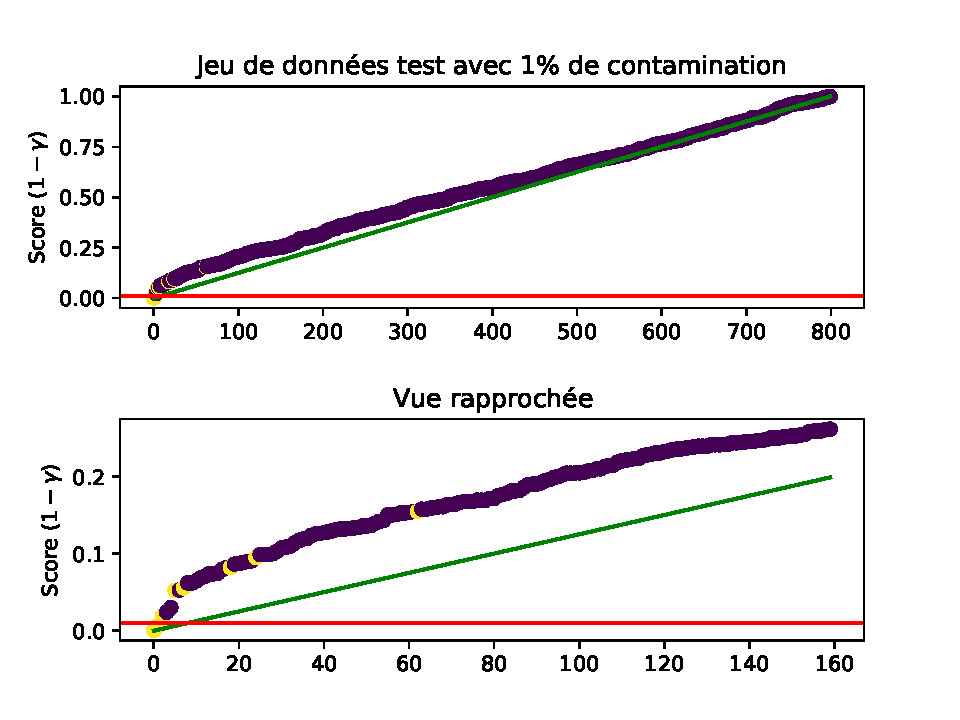
\includegraphics[width=6cm]{images/images_davae/pvalues_scenario3_moins}
		\caption{Scénario "Moins"}
	\end{subfigure}
	\begin{subfigure}{6cm}
		\centering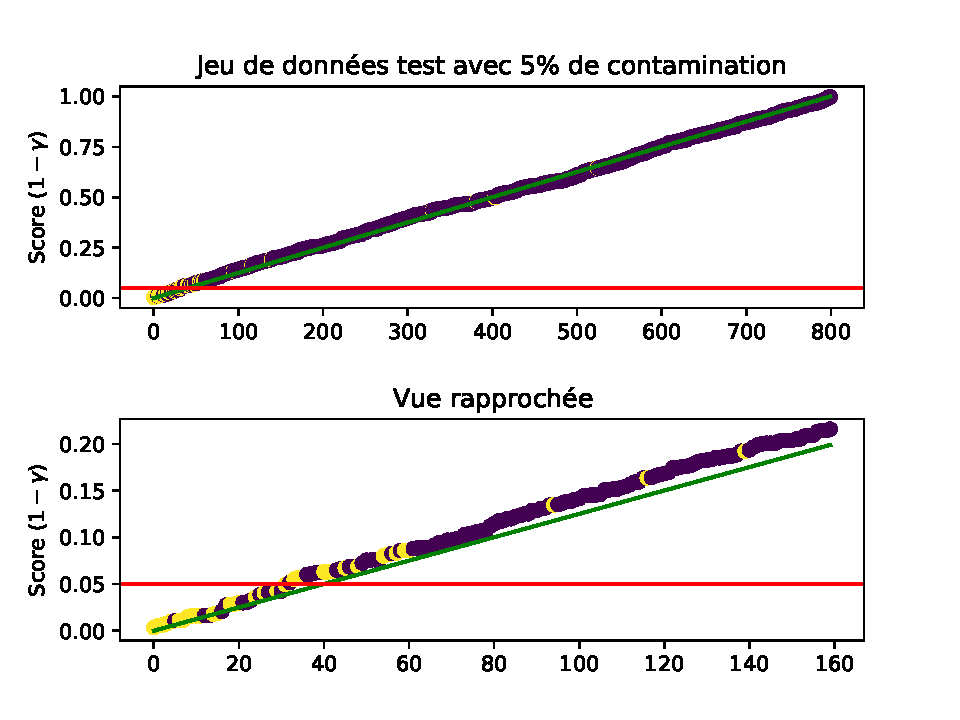
\includegraphics[width=6cm]{images/images_davae/pvalues_scenario3_egal}
		\caption{Scénario "Égal"}
	\end{subfigure}
	\begin{subfigure}{6cm}
		\centering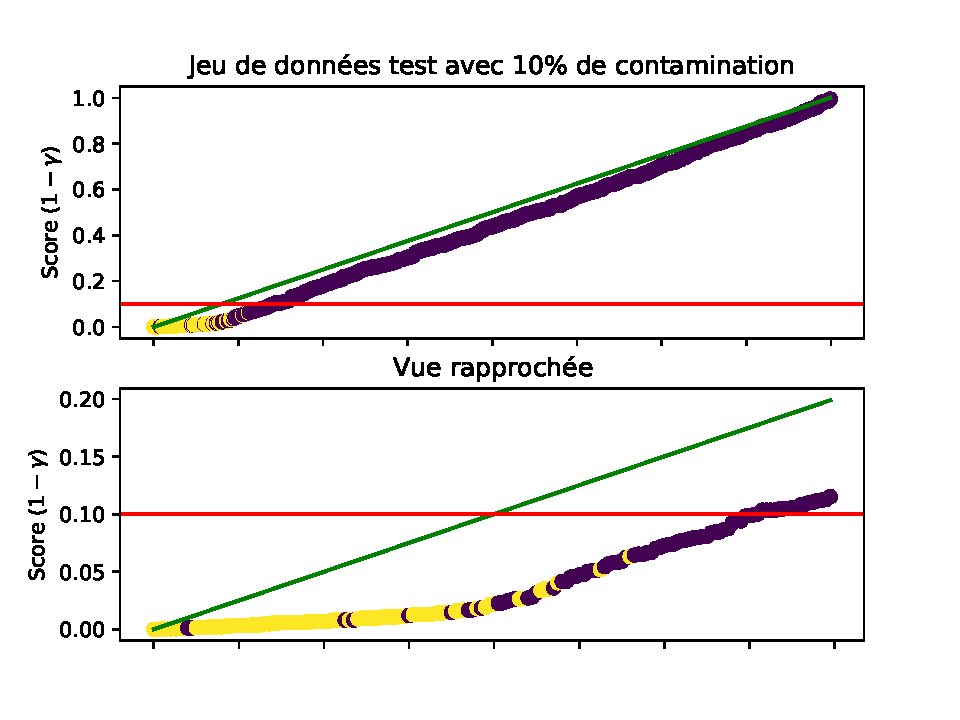
\includegraphics[width=6cm]{images/images_davae/pvalues_scenario3_plus}
		\caption{Scénario "Plus"}
	\end{subfigure}
	\caption{Graphiques illustrant les scores d'anomalies selon le scénario de contamination pour le modèle DA-VAE appliqué sur le scénario de test 1 de MNIST. Les points violets sont des observations que nous connaissons comme "normales" alors que les points jaunes sont des observations que nous connaissons comme "anormales". Dans tous les cas, le niveau de filtration $\alpha$ est défini comme le niveau de contamination dans le jeu de données de test. Pour chaque sous-figure, nous présentons une vue complète des observations du jeu de données de test ainsi qu'une vue rapprochée sur les observations situées plus à gauche de l'axe des $x$.}
	\label{fig:pvalues_scenarios_mnist}
\end{figure}

Dans les 3 sous-figures à la figure \ref{fig:pvalues_scenarios_mnist}, on peut voir que les observations "anormales", soit les points jaunes, sont principalement regroupées à gauche de l'axe des $x$, ce qui est le comportement souhaité. On remarque aussi que la segmentation est plus évidente que dans le cas de la figure \ref{fig:pvalues_scenarios}, ce qui nous permet de confirmer que la détection d'anomalies est plus performante sur ce scénario de test du jeu de données MNIST que sur le jeu de données \textit{ImageNet}. Finalement, on peut également remarquer la disposition des observations par rapport à la courbe verte. On peut tirer les mêmes constats que dans la section \ref{imagenet_results}, mais en ajoutant le fait que les positions des premières observations par rapport à la courbe verte sont encore plus prononcées dans le cas du jeu de données MNIST. Ces graphiques sont intéressants puisqu'ils pourraient servir d'outil pour interpréter la proportion d'anomalies dans le jeu de données test par rapport à la proportion présente dans le jeu de données d'entraînement. Dans la réalité, nous ne pourrions pas savoir quels observations sont des anomalies et lesquelles sont "normales". Par contre, avec la disposition de la courbe, nous pourrions savoir si le jeu de données de test contient, en proportion, moins, autant ou plus d'anomalies que le jeu de données d'entraînement.

En portant attention au niveau de filtration $\alpha$ dans les 3 différentes sous-figures de la figure \ref{fig:pvalues_scenarios_mnist}, on remarque que celui-ci semble être efficace dans le scénario de contamination "Égal". Dans les 2 autres scénarios, ce seuil ne semble pas être le niveau optimal. Toutefois, l'avantage avec cette approche de filtration est qu'il est facile de le modifier et on sait que celui-ci doit être défini dans l'intervalle $[0, 1]$.

\subsubsection{Analyses des méthodes basées sur la reconstruction} \label{mnist:reconsruction}

Dans la sous-section \ref{imagenet:reconsruction}, nous avions fais la conclusion que les méthodes basées sur la reconstruction ne permettaient pas d'obtenir de bonnes performances sur des images réelles. Dans le cas du jeu de données \textit{MNIST}, les performances de ces méthodes sont généralement supérieures à ces basées sur la représentation latente. Pour se convaincre de ces résultats, la figure \ref{fig:mnist_acp_reconstructionsa} montre des exemples d'images du jeu de données d'entraînement ayant de petites erreurs de reconstruction. Ces exemples proviennent de la méthode ACP et du scénario de test 6.  Dans le même ordre d'idées, la figure \ref{fig:mnist_acp_reconstructionsb} illustre des images provenant de la même approche, mais ayant plutôt des erreurs de reconstruction élevées. 

\begin{figure}[H]
	\centering
	\begin{subfigure}{12cm}
		\centering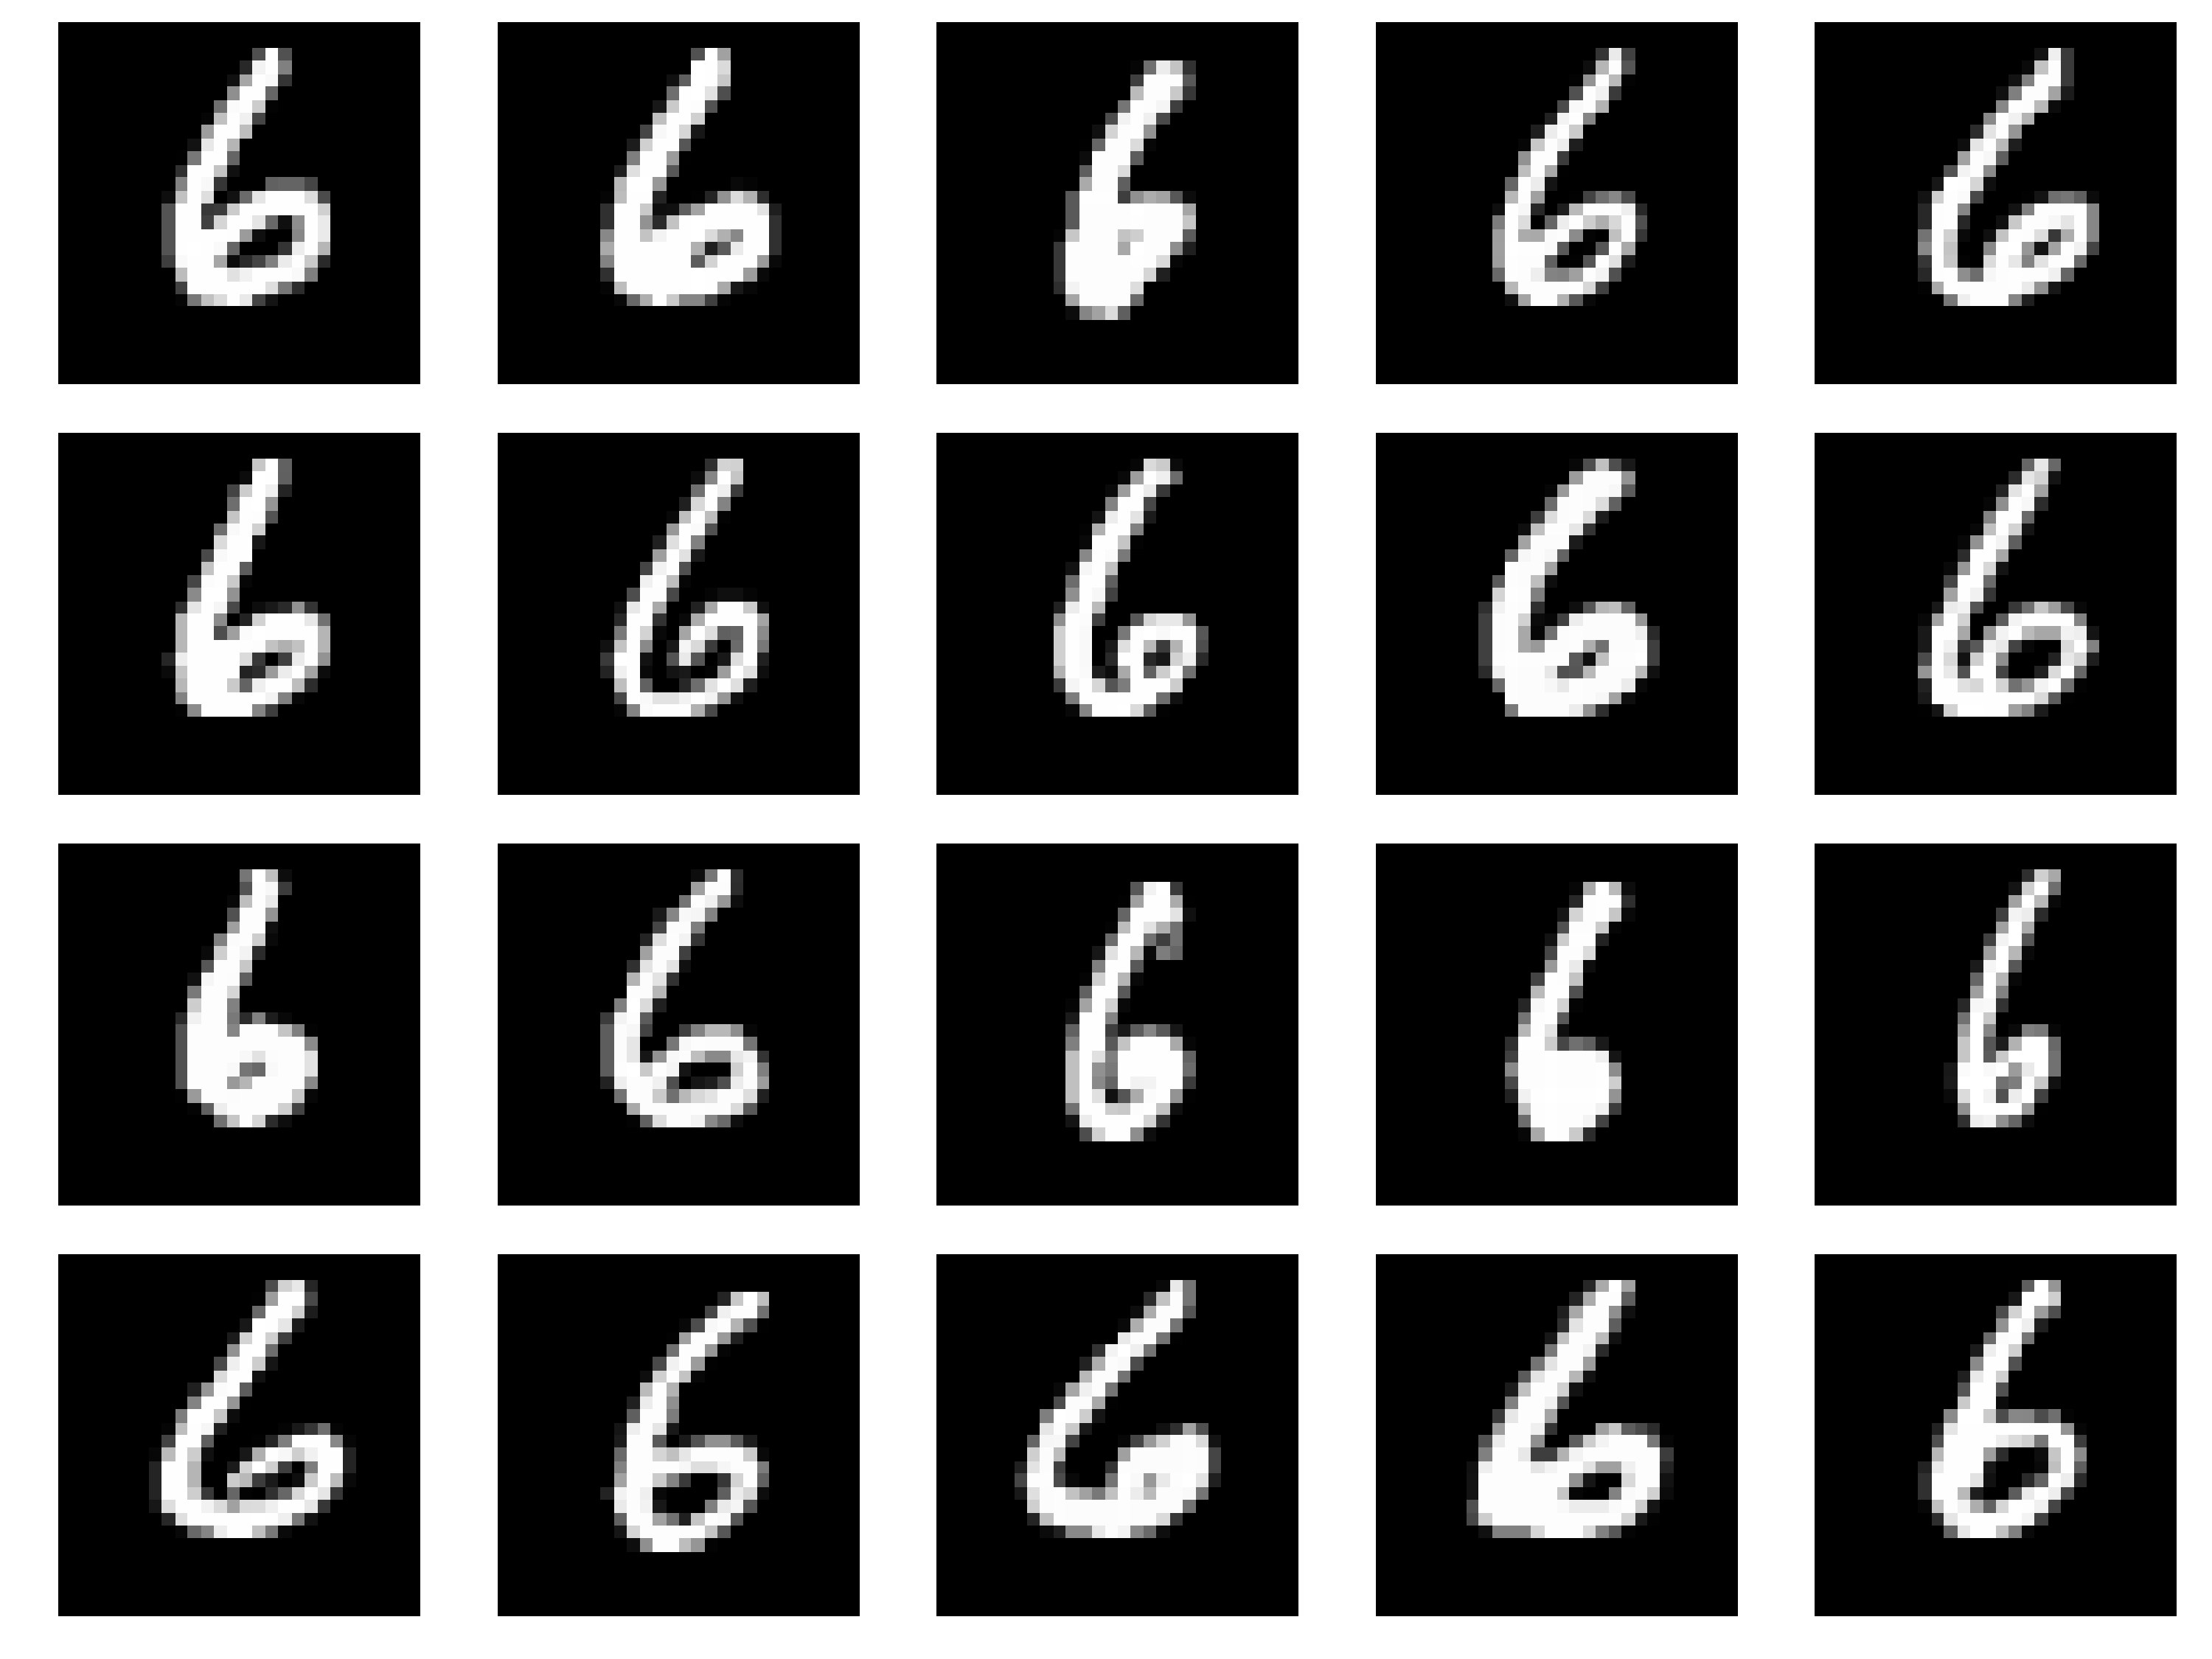
\includegraphics[width=12cm]{images/smallest_errors_mnist}
		\caption{Exemples d'images bien reconstruites}
		\label{fig:mnist_acp_reconstructionsa}
	\end{subfigure}
	\begin{subfigure}{12cm}
		\centering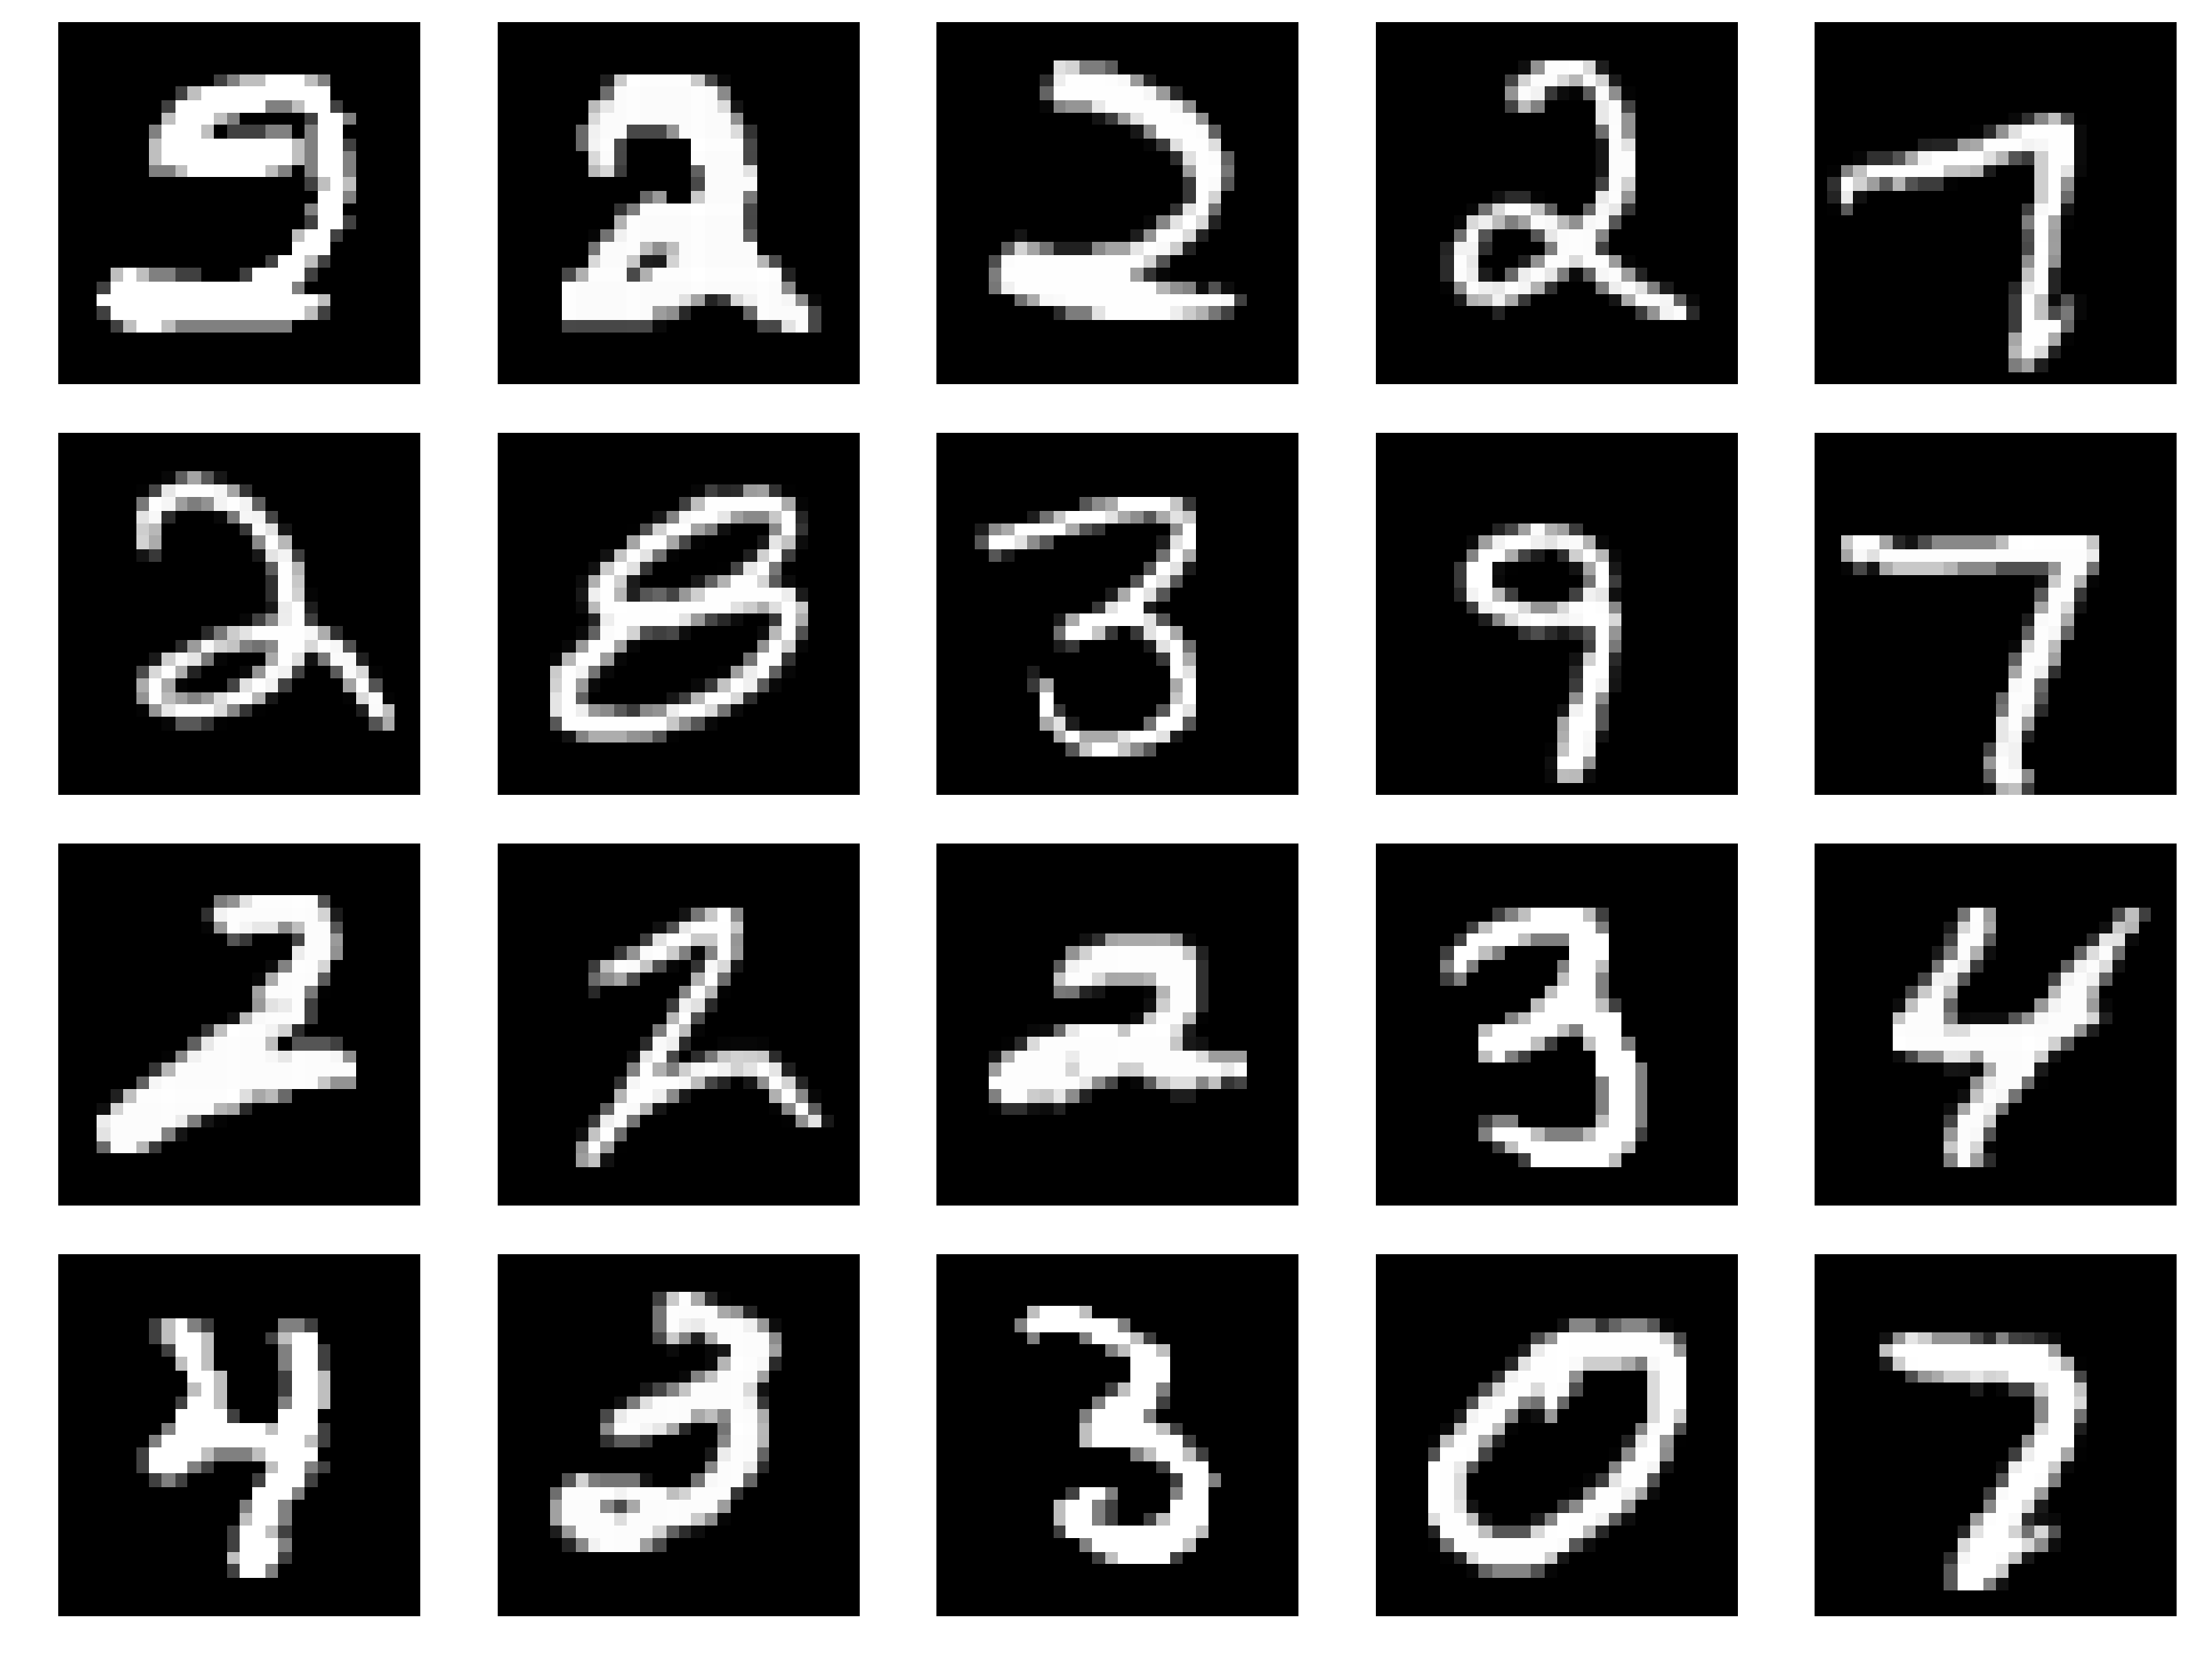
\includegraphics[width=12cm]{images/biggest_errors_mnist}
		\caption{Exemples d'images mal reconstruites}
		\label{fig:mnist_acp_reconstructionsb}
	\end{subfigure}
	\caption{Exemples d'images qui sont bien reconstruites (a) et mal reconstruites (b) selon la méthode ACP appliquée sur le jeu de données d'entraînement de \textit{MNIST}.}
	\label{fig:mnist_acp_reconstructions}
\end{figure}

En analysant la figure \ref{fig:mnist_acp_reconstructions}, on confirme en quelque sorte les bons résultats obtenus par la méthode ACP. On voit que la prémisse de base, qui dit que les images de la "normale" seront bien reconstruites, est validée. En comparaison avec le jeu de données  \textit{ImageNet}, on remarque que la classe "anormale" est beaucoup plus similaire à la classe "normale" dans le cas de \textit{MNIST}. En effet, la complexité des images est sensiblement la même. On pourrait dire que les images des deux classes proviennent de la même source, ce qui n'était pas nécessairement le cas avec notre jeu de données \textit{ImageNet}. Ainsi, on peut conclure que les méthodes basées sur la reconstruction sont performantes en détection d'anomalies lorsque les observations "anormales" partage un niveau de complexité similaire aux images "normales".

\subsubsection{Analyse des représentations latentes} 

Dans la section \ref{analyse_lat_cars}, nous avons fais l'analyse des représentations latentes par l'entremise des statistiques de distance et d'échantillons d'images. Cela nous a permit de conclure que les images "normales" avaient des statistiques de distance élevées alors que les anomalies avaient des statistiques de distance faibles. Il faut donc refaire cette analyse, mais dans le cas de \textit{MNIST}. Dans la figure \ref{fig:latentes_images_mnist}, on peut voir quelques uns des échantillons d'images du scénario de test 3 nous aidant à tirer notre conclusion. Cette fois-ci, on remarque que les observations ayant des statistiques de distance faibles proviennent de notre classe "normale", soit le chiffre "1". À l'inverse, les observations ayant des statistiques de distance élevées proviennent de notre classe "anormale", soit tous les autres chiffres. C'est d'ailleurs le cas pour les 6 différents scénarios de test.

\begin{figure}[h]
	\centering
	\begin{subfigure}{6cm}
		\centering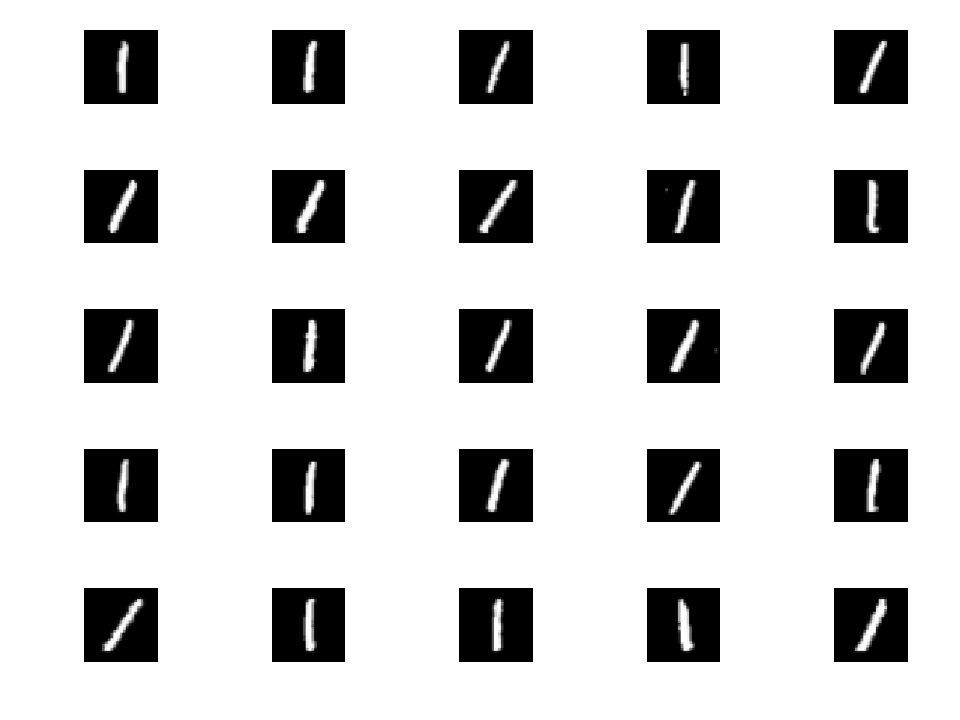
\includegraphics[width=6cm]{images/images_davae/mnist_small_distance}
		\caption{Statistiques de distance faible}
	\end{subfigure}
	\begin{subfigure}{6cm}
		\centering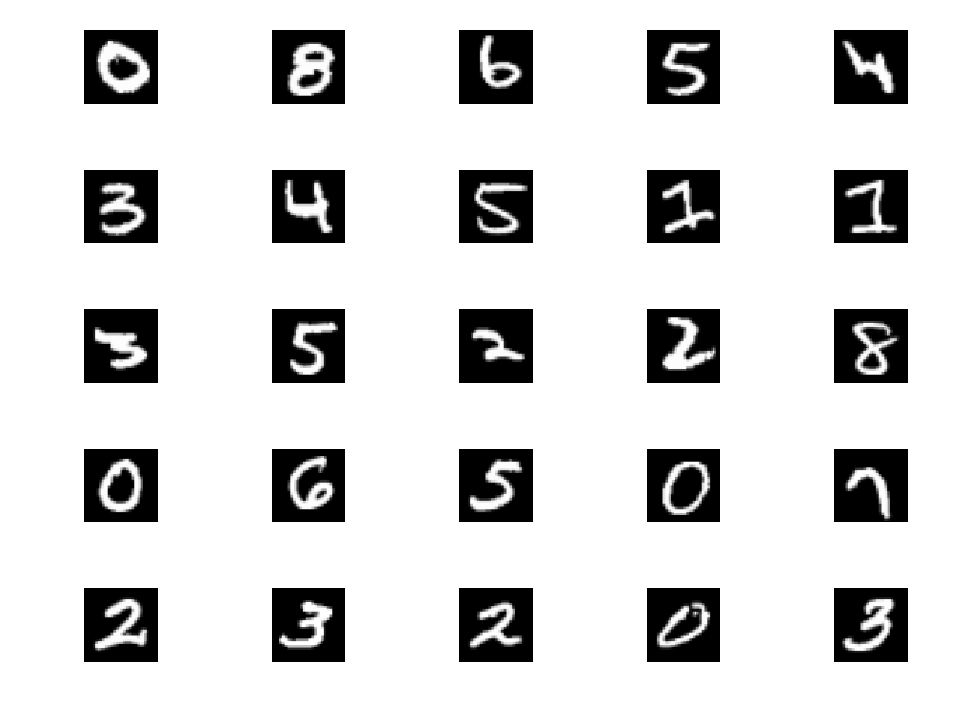
\includegraphics[width=6cm]{images/images_davae/mnist_large_distance}
		\caption{Statistiques de distance élevées}
	\end{subfigure}
	\caption{Échantillons d'images provenant du jeu de données d'entraînement ayant des statistiques de distance faibles (a) et élevées (b) pour le scénario de test 3 ("Plus") du jeu de données \textit{MNIST}.}
	\label{fig:latentes_images_mnist}
\end{figure}

De cette manière, il est possible de conclure que nous nous retrouvons plutôt dans le premier scénario décrit (voir les deux scénarios décrits à la sous-section \ref{liste_scenarios}), soit celui où les représentations latentes des observations "normales" sont plus près de la $N(0,I)$. C'est donc le scénario inverse par rapport aux expérimentations faites sur \textit{ImageNet}. On peut d'ailleurs confirmer cette conclusion dans la figure \ref{fig:mnist_latent_stats}, où l'on peut voir que les vecteurs $\boldsymbol{\mu}$ et $\boldsymbol{\sigma}$ moyens des observations "normales" sont plus près des paramètres de moyenne et d'écart-type de la $N(0,I)$.

\begin{figure}[H]
	\centering
	\begin{subfigure}{12cm}
		\centering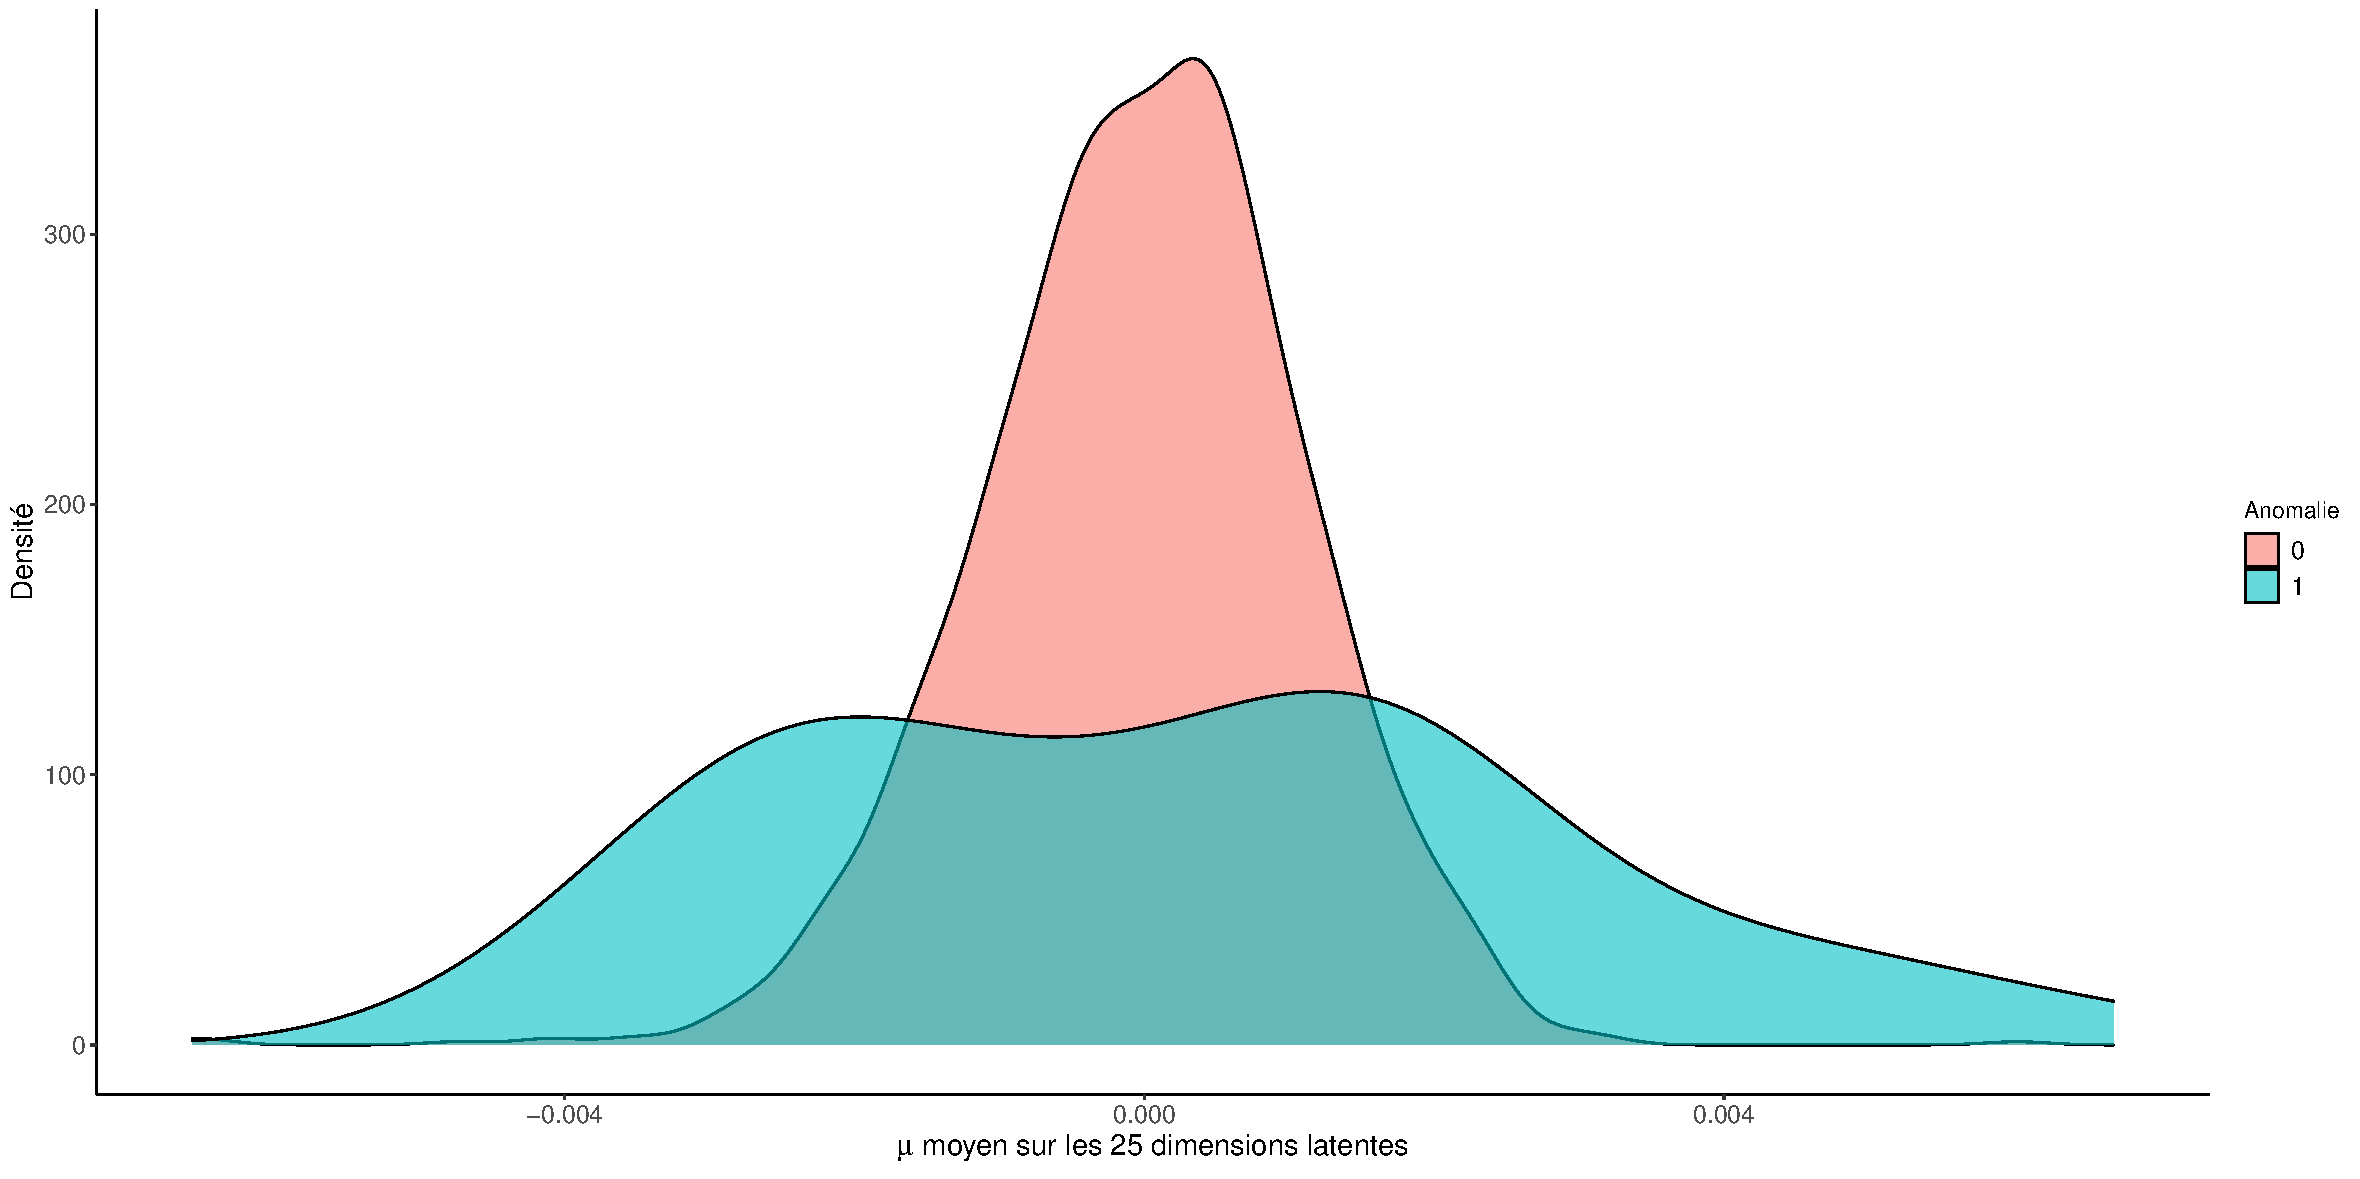
\includegraphics[width=12cm, height=6cm]{images/latent_stats/plot_mu_mnist}
		\caption{Distribution des $\boldsymbol{\mu}$ moyens}
	\end{subfigure}
	\begin{subfigure}{12cm}
		\centering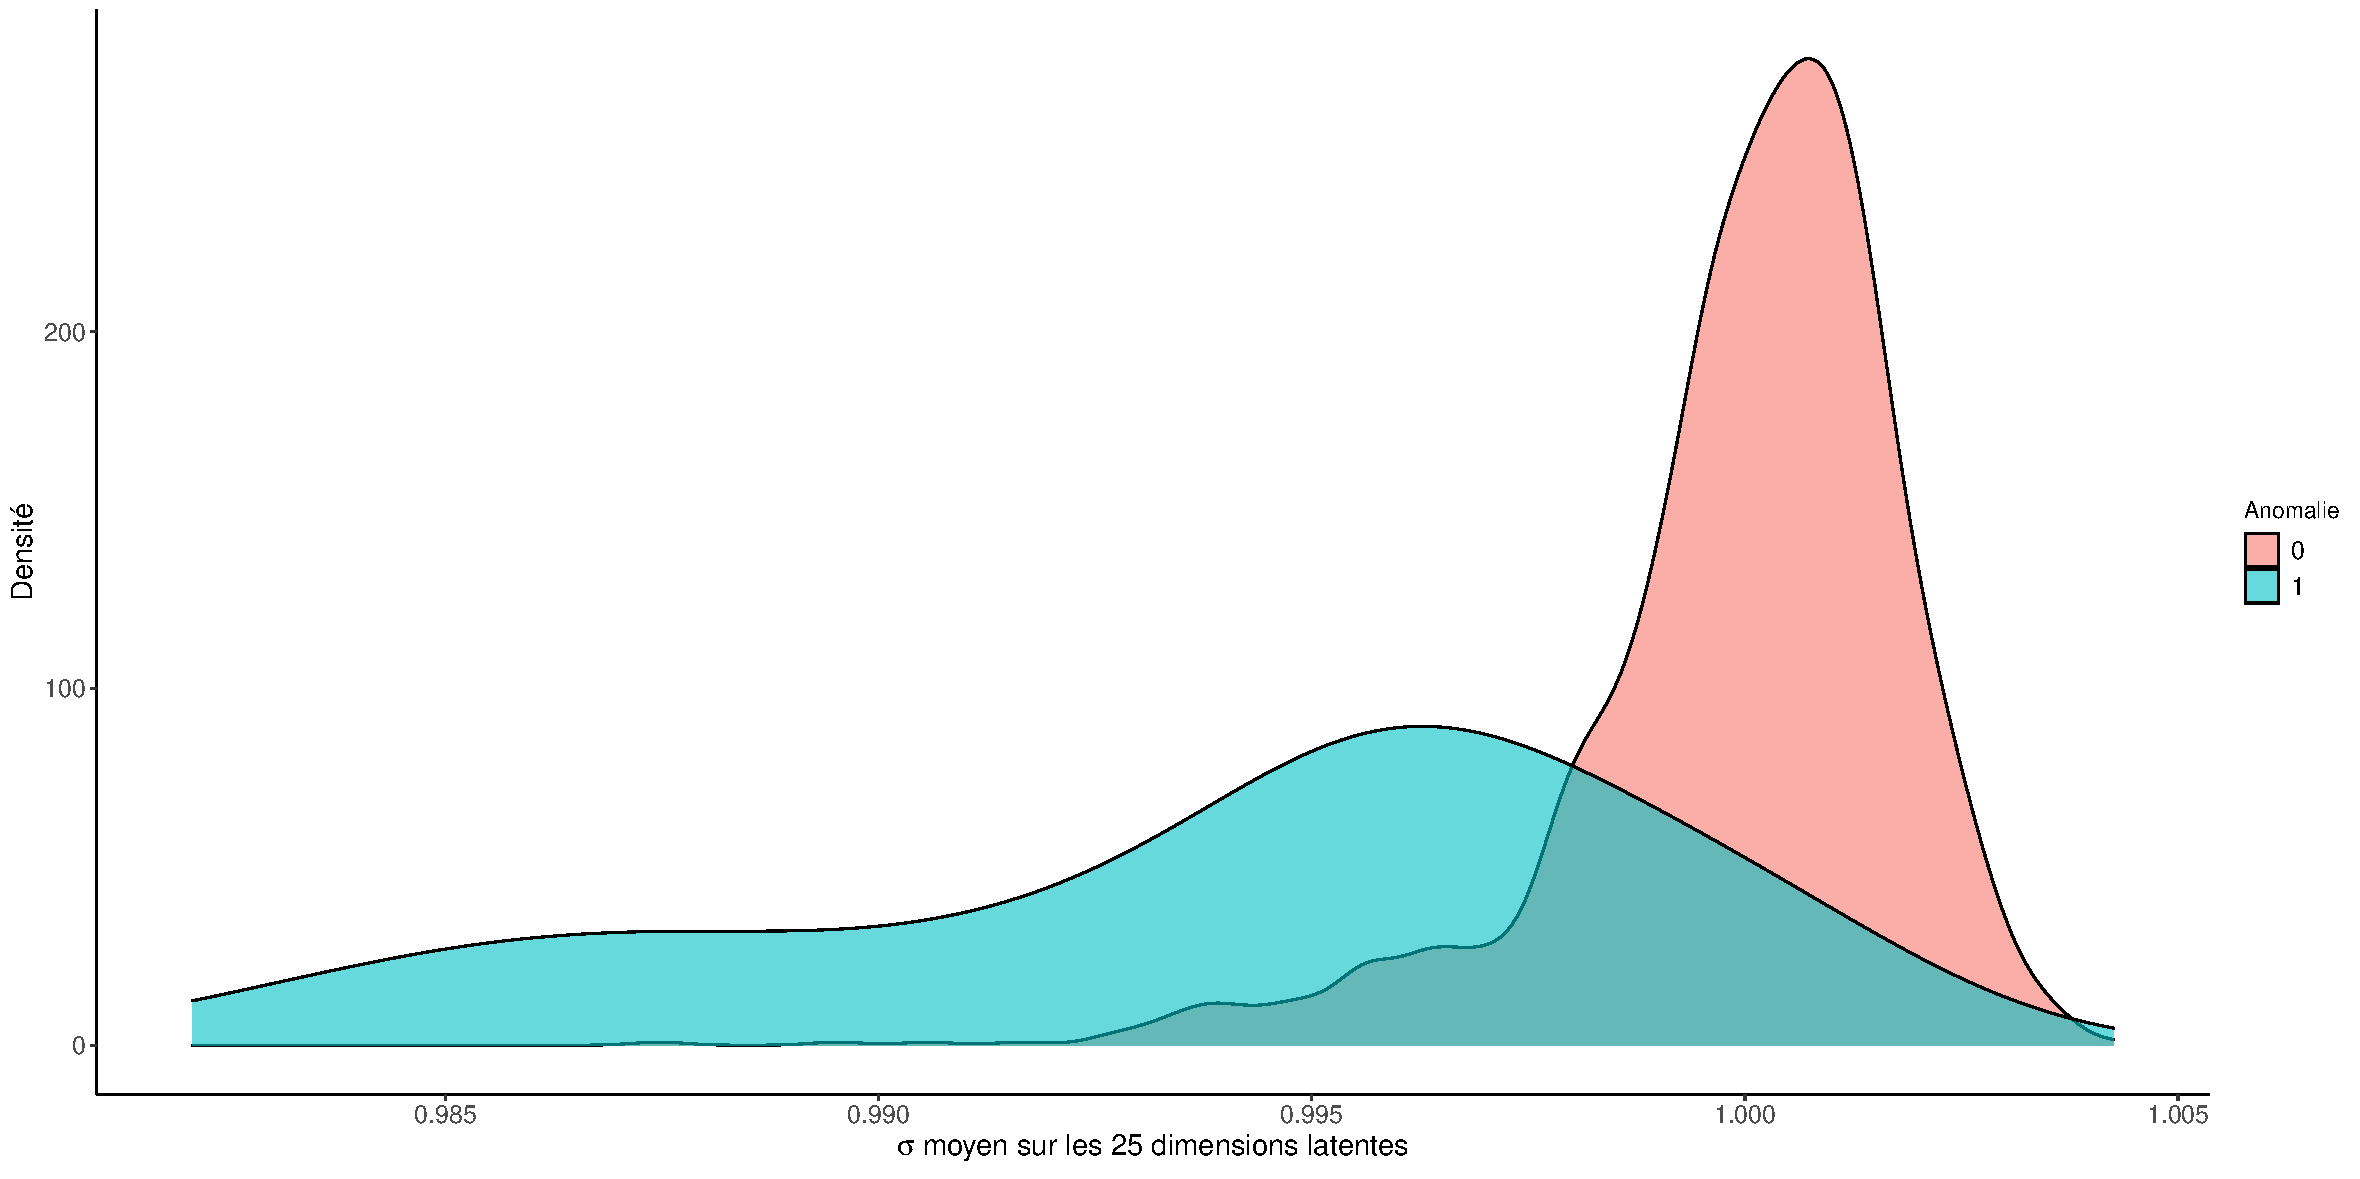
\includegraphics[width=12cm, height=6cm]{images/latent_stats/plot_sigma_mnist}
		\caption{Distribution des $\boldsymbol{\sigma}$ moyens}
	\end{subfigure}
	\caption{Moyenne des $\boldsymbol{\mu}$ et $\boldsymbol{\sigma}$ des représentations latentes du jeu de données d'entraînement sur le jeu de données \textit{MNIST}.}
	\label{fig:mnist_latent_stats}
\end{figure}

\begin{figure}[htb]
	\centering
	\centering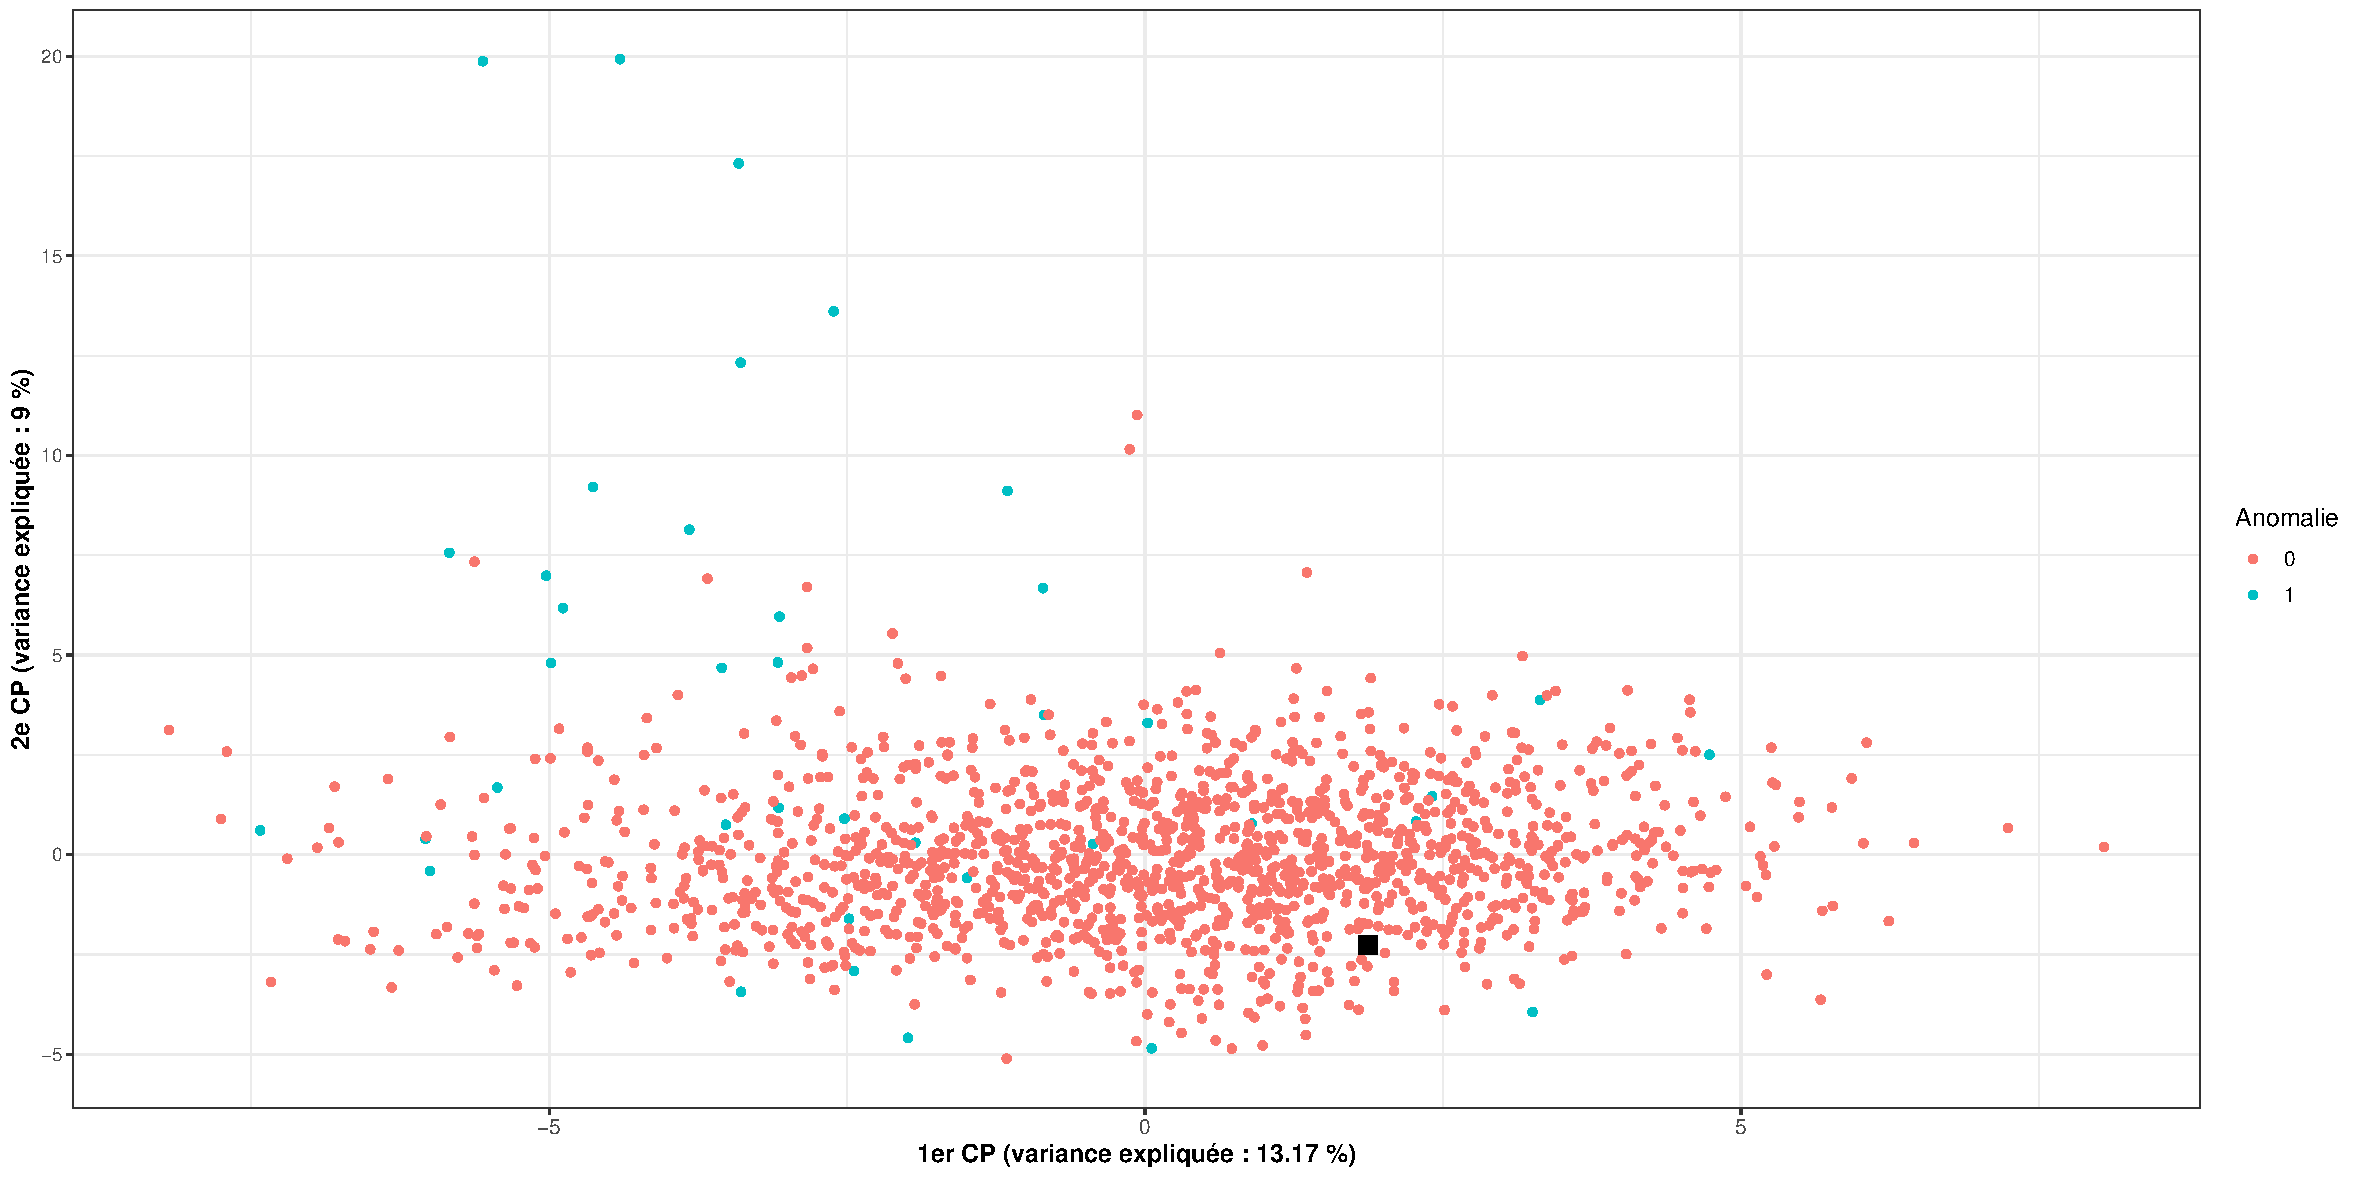
\includegraphics[width=\linewidth]{images/plot_pca_mnist}
	\caption{Graphique des 2 premières composantes principales réalisé sur les vecteurs $\boldsymbol{\mu}$ et $\boldsymbol{\sigma}$ du jeu de données d'entraînement \textit{MNIST} appliqué sur le scénario de test 3 et le scénario de contamination "Plus".}
	\label{fig:pca_mnist}
\end{figure}

Dans la figure \ref{fig:pca_mnist}, on peut voir le résultat d'une analyse en composantes principales appliquée sur les vecteurs $\boldsymbol{\mu}$ et $\boldsymbol{\sigma}$. Cette figure nous permet de visualiser en 2 dimensions, les représentations latentes apprises sur le jeu de données d'entraînement du scénario de test 3 et du scénario de contamination "Plus". Si on compare avec la figure \ref{fig:pca_cars} qui fait référence au jeu de données \textit{ImageNet}, la séparation des anomalies et des observations "normales" est beaucoup moins évidente. Cependant, les 2 premières composantes principales n'expliquent même pas 25\% de la variabilité totale de la représentation latente. En se basant sur cette projection, les "anomalies" semblent être plus éloignées du carré noir, qui représente la projection dans cet espace du point $(\boldsymbol{0_{m}}, \boldsymbol{1_{m}})$. Cette conclusion concorde avec l'analyse de la figure \ref{fig:mnist_latent_stats}. Étant donné que l'analyse en composantes principales ne permet pas de voir de clairement la séparation des anomalies et des observations "normales" dans un espace en deux dimensions, nous avons explorer une autre avenue afin d'obtenir cette visualisation. Pour ce faire, nous avons fait un nouvel entraînement de la méthode DA-VAE, mais cette fois-ci avec seulement deux dimensions latentes (au lieu de 25). Cette configuration nous permettra de visualiser les vecteurs $\boldsymbol{\mu}$ et $\boldsymbol{\sigma}$ dans un espace à deux dimensions sans avoir à faire de réduction de dimensionnalités. Dans la figure \ref{fig:mnist_latent_2d}, on peut désormais voir de manière plus évidente que les représentations latentes des observations "normales" sont plus près du point $(\boldsymbol{0_{m}}, \boldsymbol{1_{m}})$.

\begin{figure}[H]
	\centering
	\begin{subfigure}{6cm}
		\centering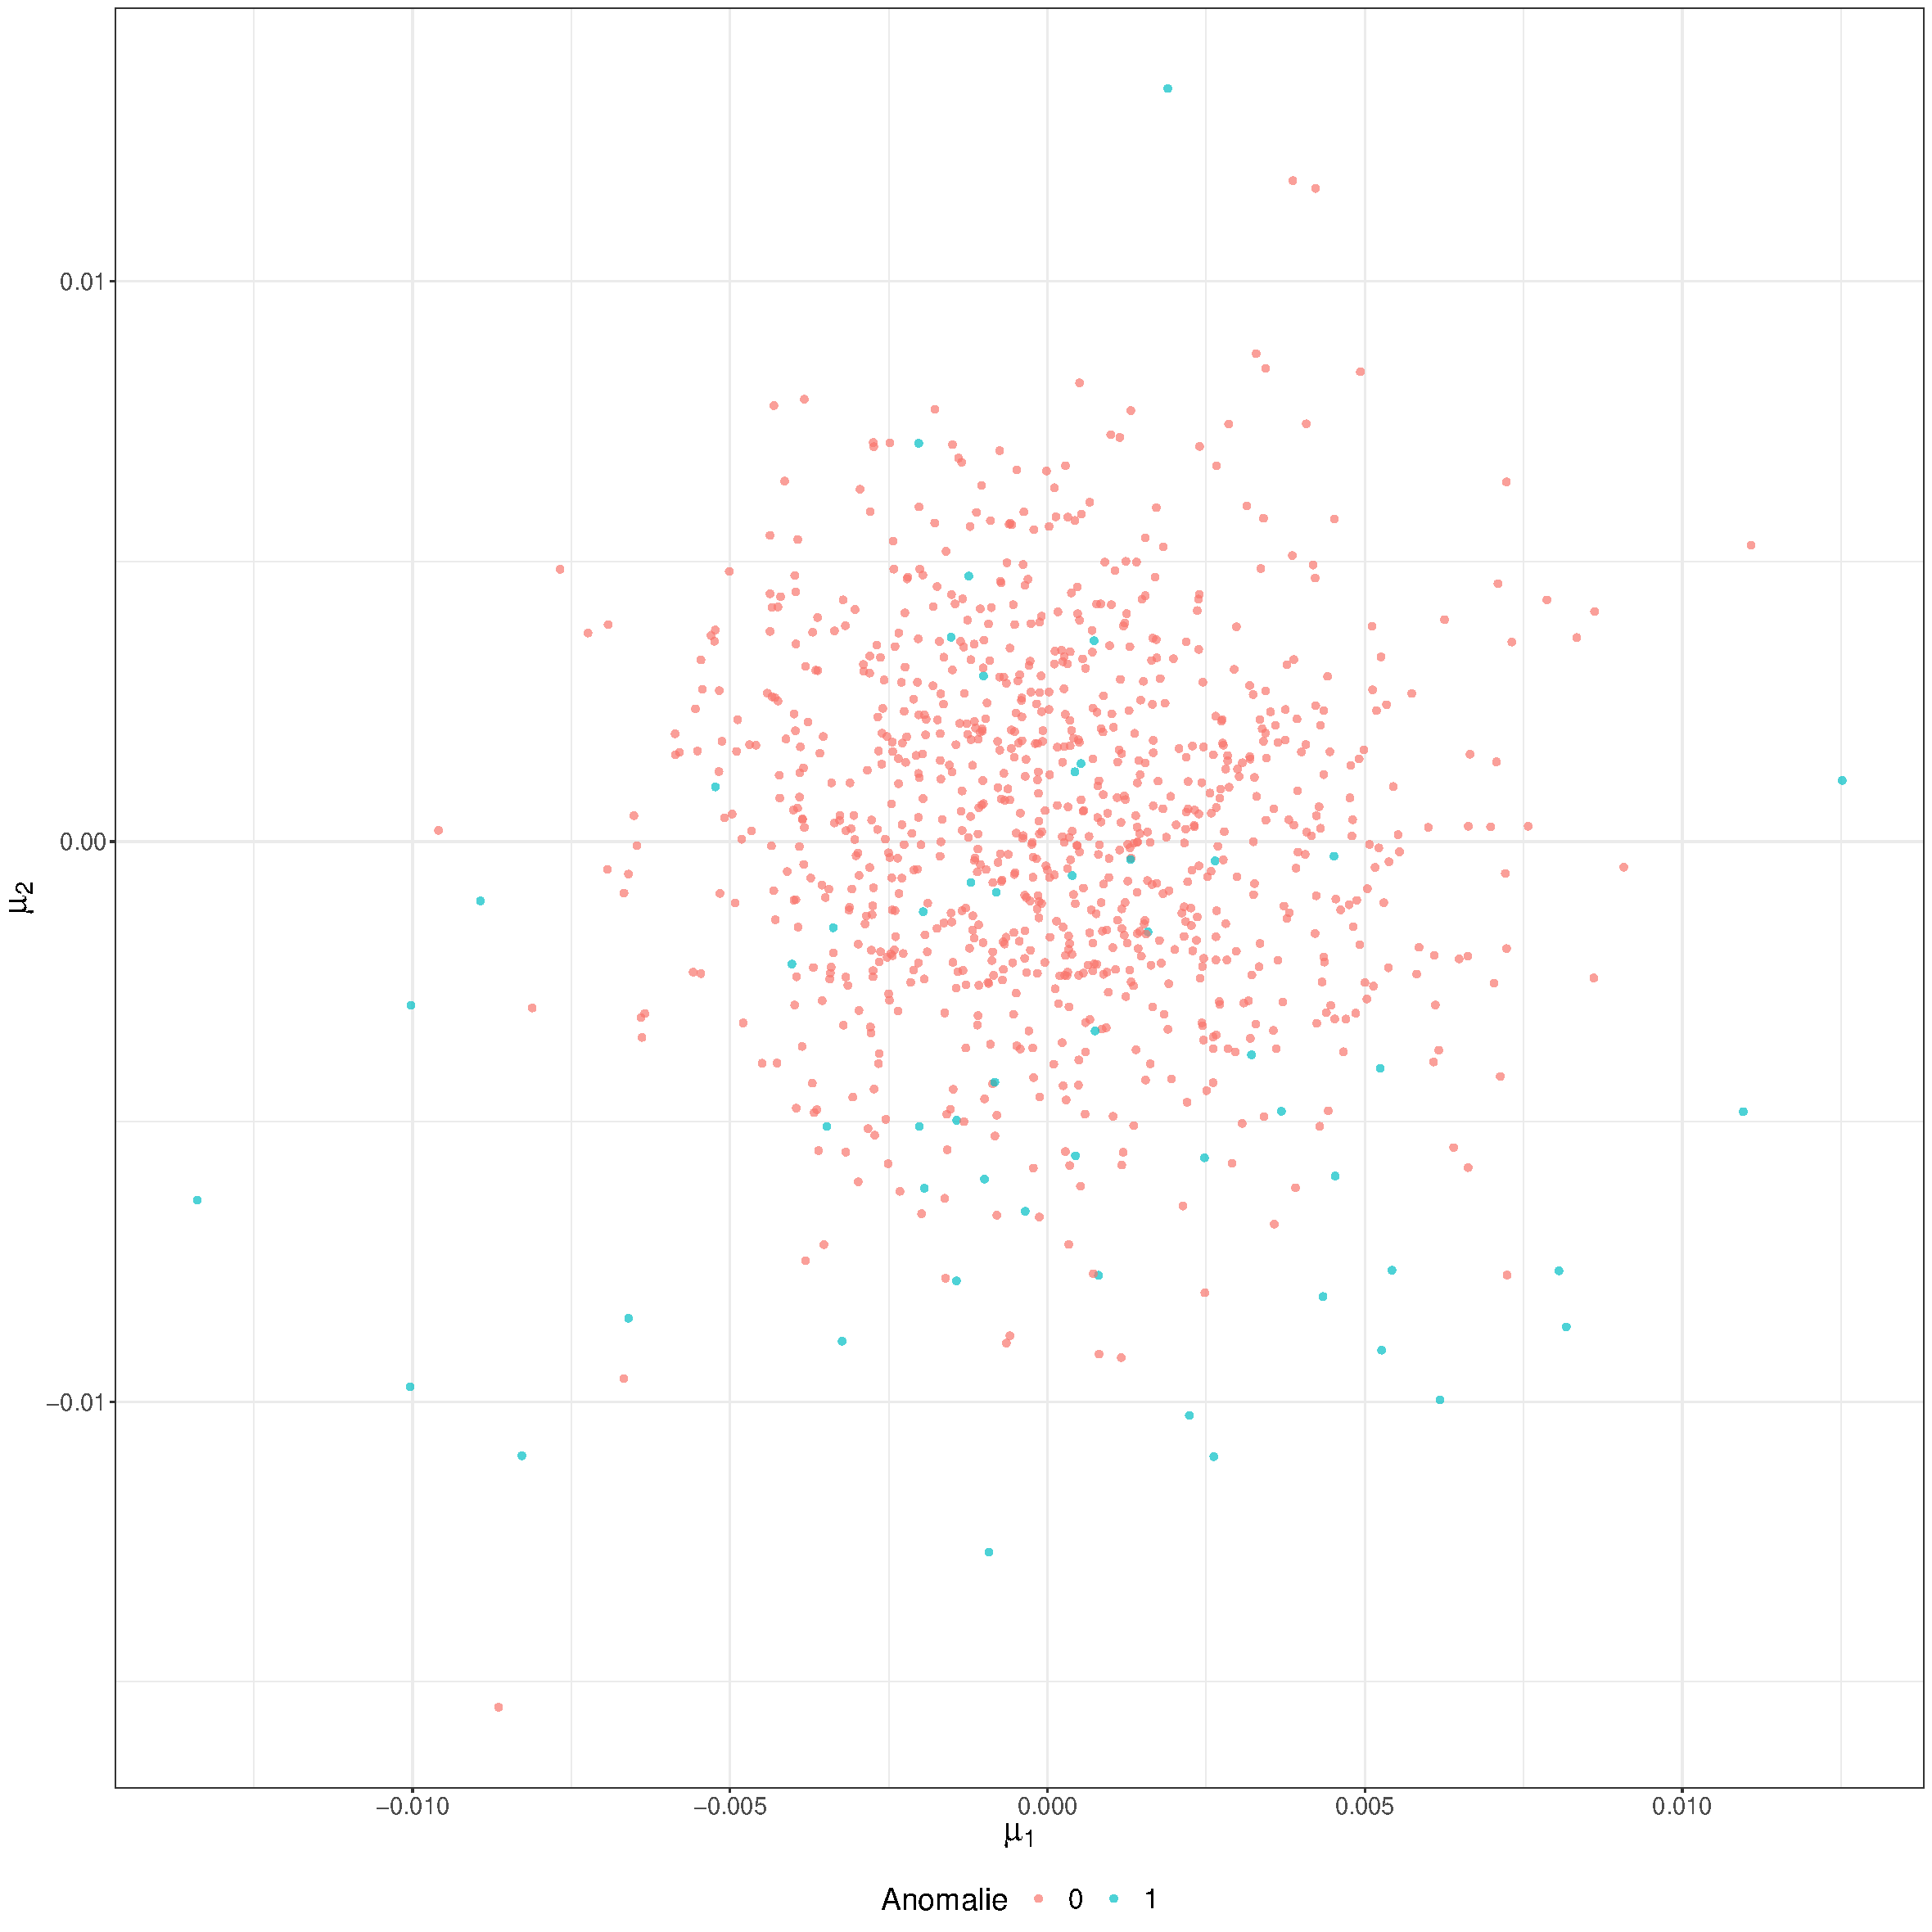
\includegraphics[width=6cm, height=6cm]{images/latent_stats/mnist_mu_2d}
		\caption{Distribution de $\mu_1$ et $\mu_2$}
	\end{subfigure}
	\begin{subfigure}{6cm}
		\centering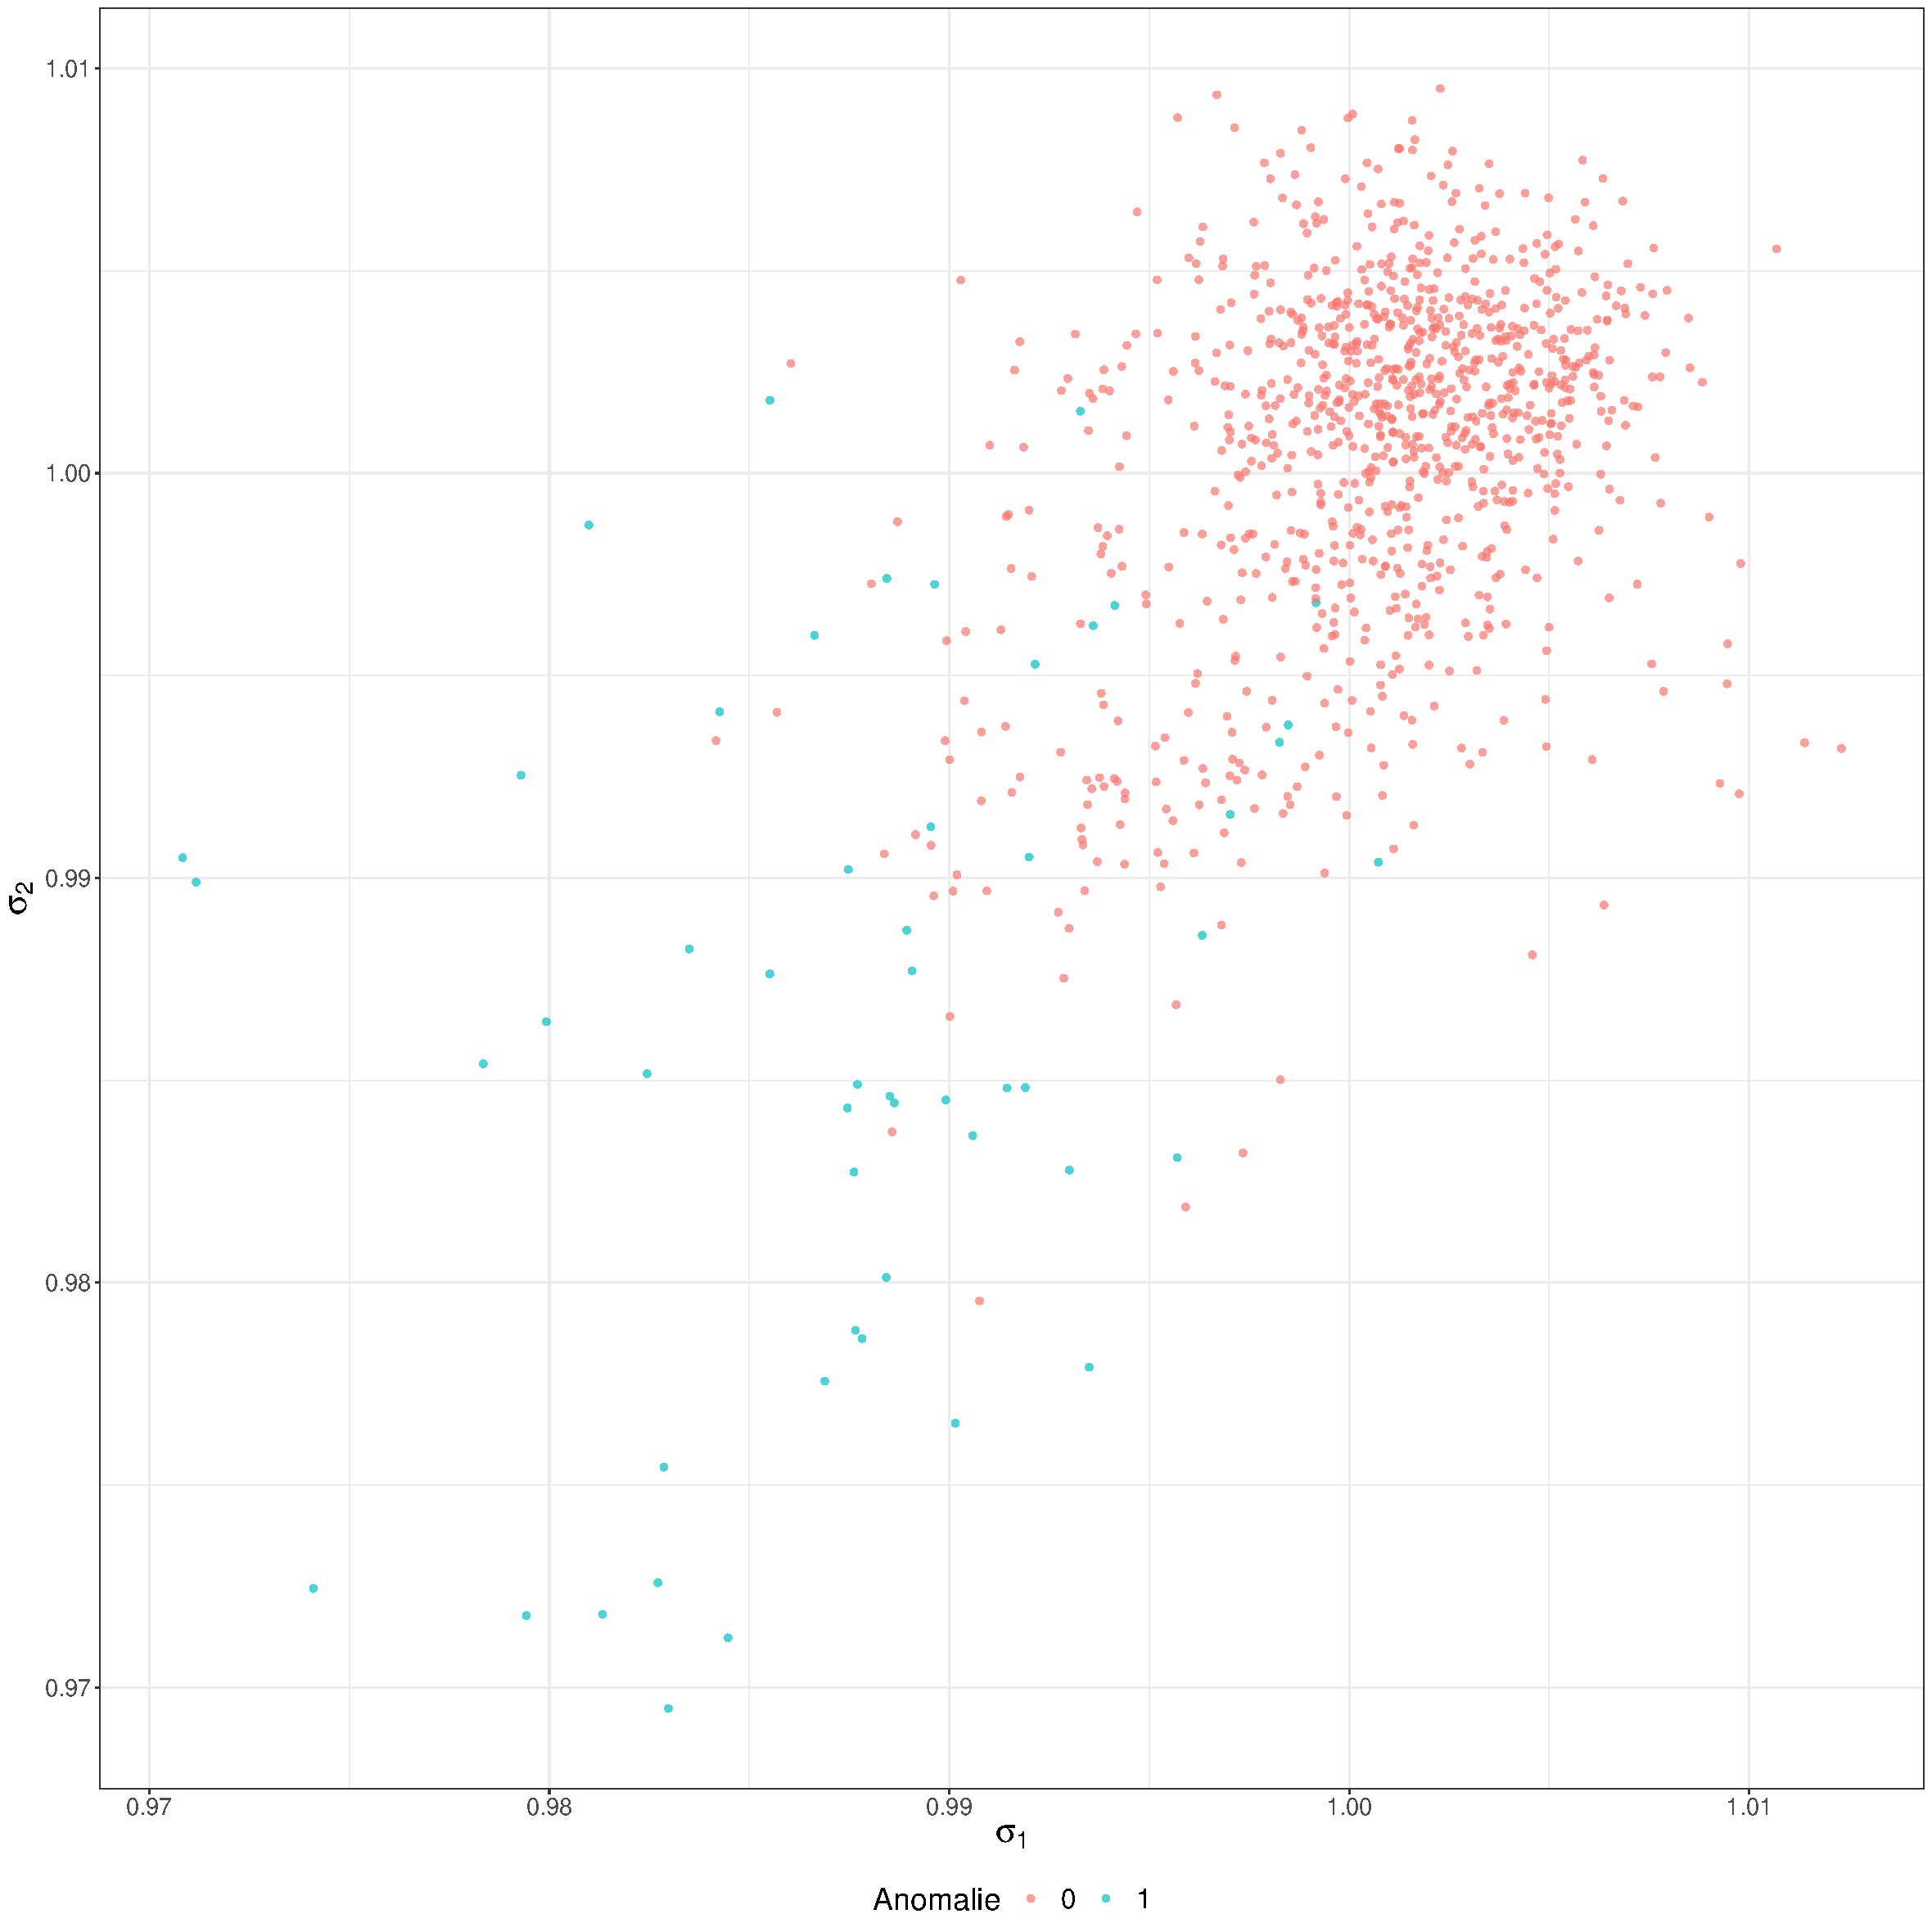
\includegraphics[width=6cm, height=6cm]{images/latent_stats/mnist_sigma_2d}
		\caption{Distribution de $\sigma_1$ et $\sigma_2$}
	\end{subfigure}
	\caption{Distribution des vecteurs $\boldsymbol{\mu}$ et $\boldsymbol{\sigma}$ pour le modèle DA-VAE entraîné avec un espace latent à deux dimensions sur le scénario de test 3 et le scénario de contamination "Égal" du jeu de données \textit{MNIST}.}
	\label{fig:mnist_latent_2d}
\end{figure}

Dans la figure \ref{fig:mnist_latent_2d}, nous avons utilisé un entraînement sur scénario de test 3 avec le scénario de contamination "Égal". Afin de pouvoir mieux observer la distribution des points, nous avons conservé seulement 500 observations, choisies aléatoirement, du jeu de données d'entraînement. Comme nous l'avions remarqué dans la figure \ref{fig:mnist_latent_stats}, le vecteur latent $\boldsymbol{\sigma}$ semblent être plus discriminant que le vecteur latent $\boldsymbol{\mu}$.

\subsubsection{Analyse de la perte en entraînement}

Dans la figure \ref{fig:mnist_kld_perc}, on peut voir la composition de la perte à chacune des itérations de l'entraînement. On peut voir que la proportion de la composante de perte de Kullback-Leibler suit le même patron qu'à la figure \ref{fig:cars_kld_perc}. Cependant, la proportion atteint un maximum beaucoup plus élevé que dans le cas du jeu de données provenant de \textit{ImageNet}. Encore une fois, il est rassurant de voir que la composition réelle de la perte soit cohérente avec notre horaire établi pour l'hyperparamètre $\beta$. 

\begin{figure}[h]
	\centering
	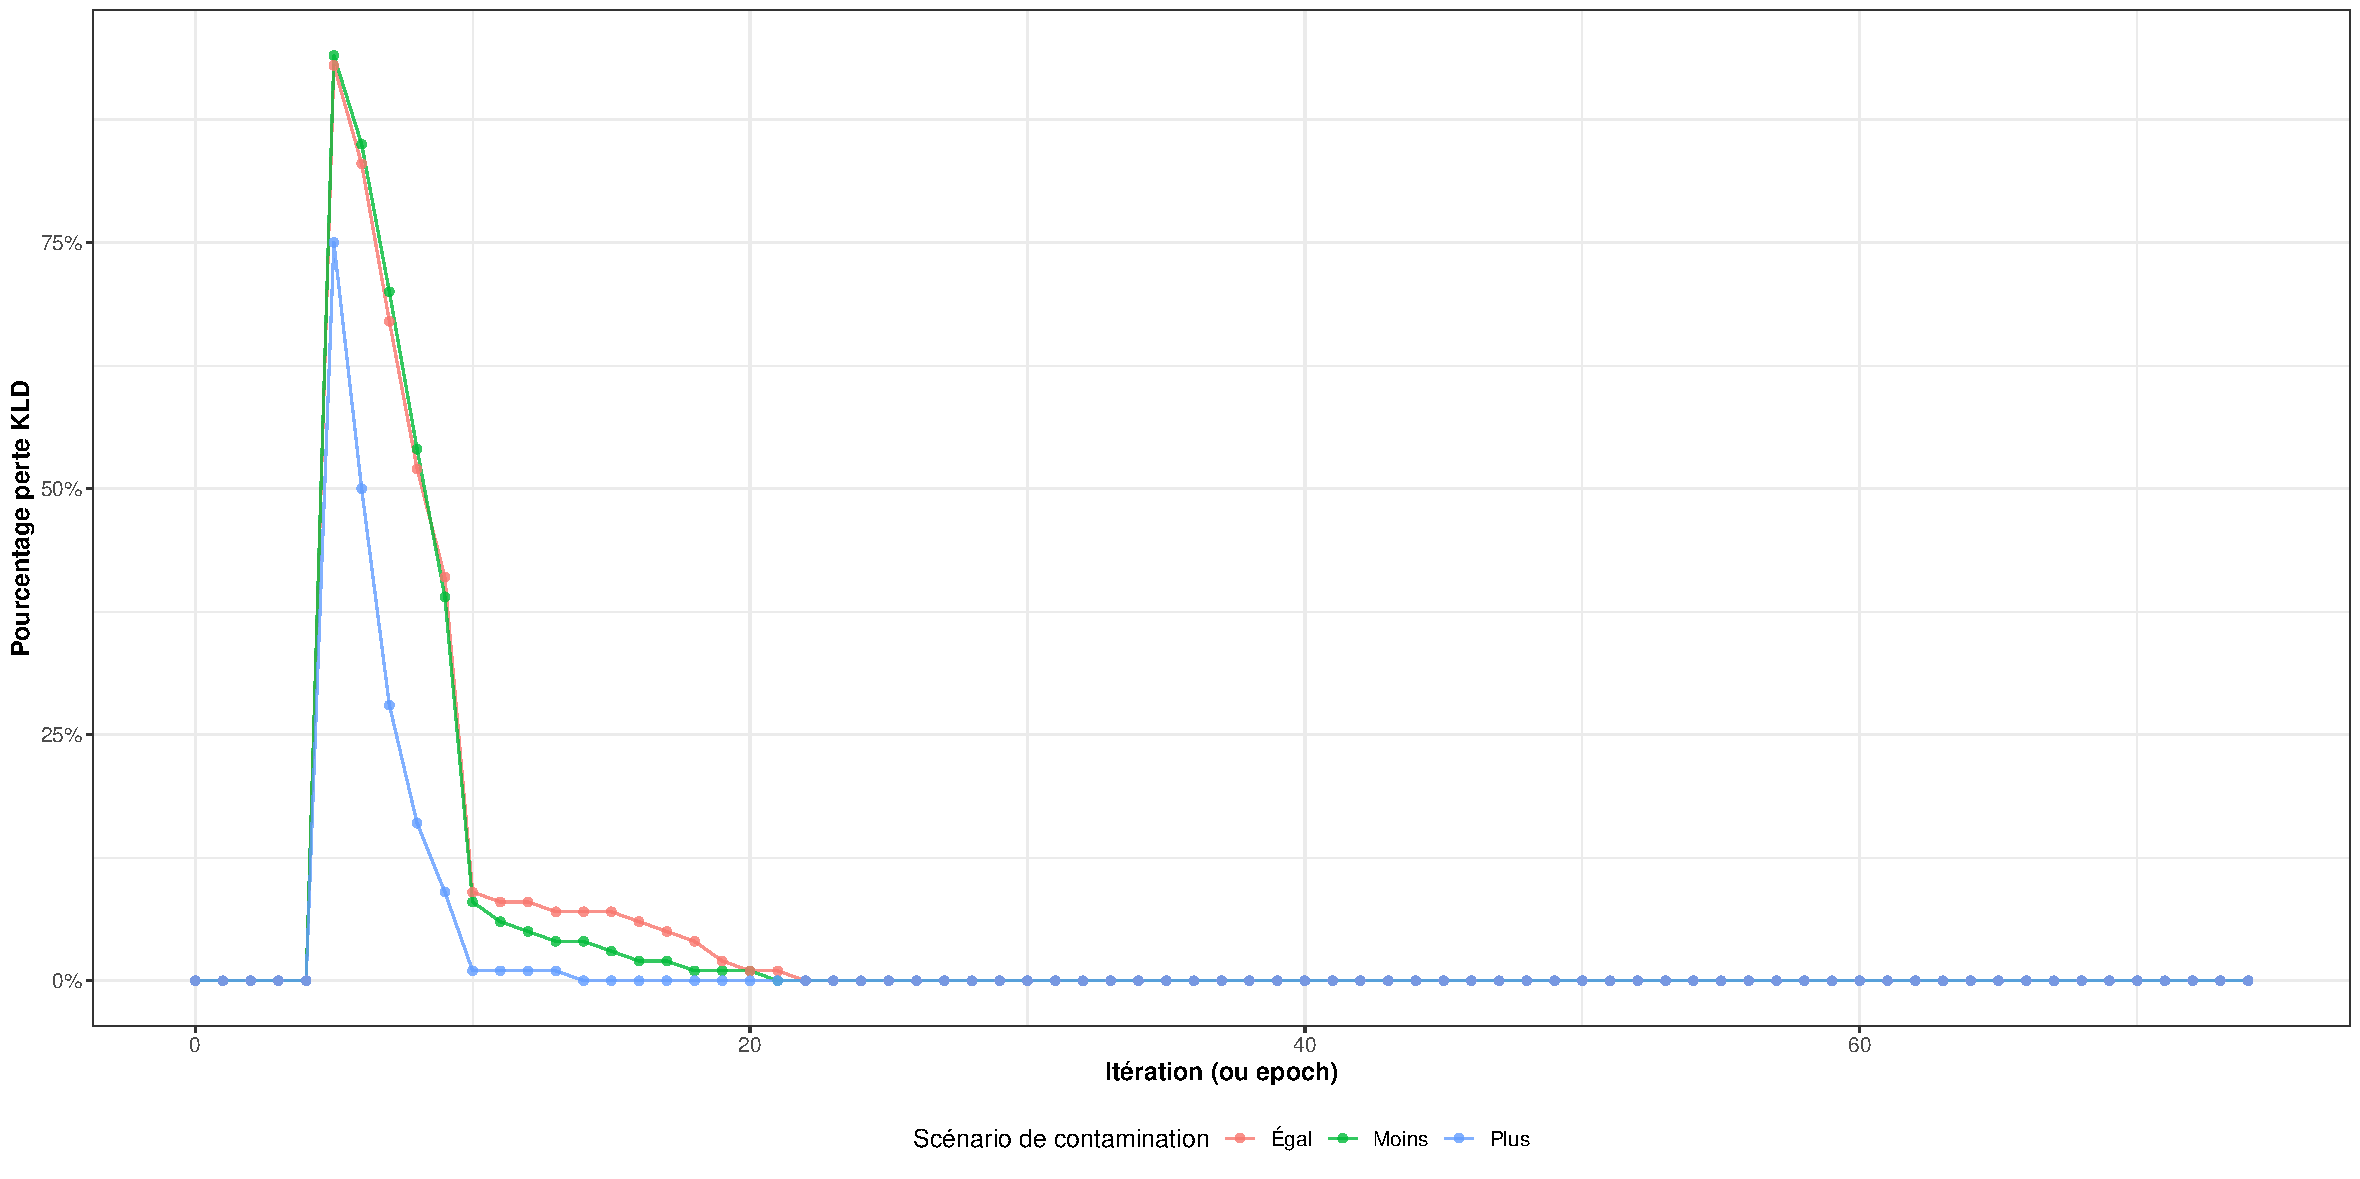
\includegraphics[width=\linewidth]{images/kld_mnist_scenario_3.pdf}
	\caption{Pourcentage du critère de Kullback-Leibler dans la perte totale selon l'itération d'entraînement et le scénario de contamination. Ces résultats sont tirés du scénario de test 3, où le chiffre "1" est considéré comme la classe "normale" et tous les autres sont considérés dans la classe "anormale".}
	\label{fig:mnist_kld_perc}
\end{figure}

